%!TEX root = ../report.tex

\begin{document}
    \chapter{Experiments and Results}
    %In this chapter, we will discuss about the experiments conducted for out-of-distribution (OOD) detection on RandLA-Net using uncertainty techniques such as deep ensembles and flipout.
    %These experiments were conducted on Semantic3D dataset as training in-distribution (ID) dataset and two datasets particularly S3DIS and Toronto3D are used as OOD datasets. 
    %The detailed description about datasets can be found in Chapter \textcolour{red}{cite here}, about RandLA-Net in Section \textcolour{red}{cite here}, and about deep ensembles and flipout in Section \textcolour{red}{cite here}
    %The list of experiments conducted to acheive OOD detection are as follows:
    This chapter discusses the experiments conducted for Out-Of-Distribution (OOD) detection on RandLA-Net using quantified uncertainty from Deep Ensembles and Flipout.
    A detailed discussion about RandLA-Net, Deep Ensembles and Flipout can be found in Chapter~\ref{chapter:methodology}. In this chapter, we first discuss the training results of RandLA-Net using deep ensembles and flipout on Semantic3D as an In-Distribution (ID) dataset.
    Furthermore, we compare the Maximum Softmax Probability (MSP) as in \cite{hendrycks2016baseline_MSP} and entropy values for the proposed OOD benchmark datasets Semantic3D vs S3DIS and Semantic3D vs Semantic3D without colour.
    Finally, we visualize and evaluate the performance of OOD detection using the AUROC score.

%%%%%%%%%%%%%%%%%%%%%%%%%%%%%%%%%%%%%%%%%%%%%%%%%%%%%%%%%%%%%%%%%%%%%%%%%%%%%%%
    %%%%%% Deep ensmebles performance %%%%%%
    \section{Deep Ensembles-Semantic3D}
    \label{sec:deepensemble_train}
    In this experiment, we trained 20 models of RandLA-Net over the Semantic3D dataset using random initializations with the experimental setup described in Section~\ref{sec:de_setup}.
    The predictions from these 20 individual models are then averaged to compute the final predictions.
    The evaluation results of the Deep Ensembles are described in Table~\ref{tab:ensemble_eval} using meanIoU, per-class IoU and Accuracy.
    The predictions from the Deep Ensembles are depicted in Figure~\ref{fig:deepensemble_vis_sem3d} and Figure~\ref{fig:deepensemble_improv}.
    \begin{table}[h!]
        \resizebox{\textwidth}{!}{%
        \begin{tabular}{c|c|cccccccc|c}
        %\textbf{\#Ensembles} & \textbf{MeanIOU} & \textbf{Accuracy} & \textbf{Manmadeterrain} & \textbf{Naturalterrain} & \textbf{Highvegetation} & \textbf{Lowvegetation} & \textbf{Buildings} & \textbf{Hardscapes} & \textbf{Scanningartifacts} & \textbf{Cars} \\ \hline
        & & \multicolumn{7}{c}{\textbf{IoU per-class}} & \\ \hline
        \textbf{Ensemble size} & \textbf{meanIoU} & \textbf{C1} & \textbf{C2} & \textbf{C3} & \textbf{C4} & \textbf{C5} & \textbf{C6} & \textbf{C7} & \textbf{C8} & \textbf{Accuracy} \\ \hline
        1& 68.19& 94.55& 81.19& 84.67& 29.43& 81.37& 18.85& 64.74& 90.74& 88.78 \\
        5& 69.51& 94.73& 81.92& 84.42& 28.05& \textbf{86.41}& 28.50& 61.03& 91.03& 90.04 \\
        10& 69.97& 95.25& 83.73& 86.63& 30.36& 84.13& 18.60& \textbf{66.01}& 92.61& 89.94 \\
        15& 70.32& 95.27& 83.54& \textbf{88.22}& \textbf{32.19}& 84.82& 26.17& 61.67& 90.75& \textbf{90.57} \\
        20& \textbf{70.80}& \textbf{95.55}& \textbf{84.11}& 86.65& 29.60& 85.41& \textbf{29.58}& 62.47& \textbf{93.06}& 90.56 \\
        \end{tabular}%
        }
        \caption{Illustration of performance of RandLA-Net on Semantic3D over ensemble size. meanIOU, IOU per-class and overall accuracy are represented here.
        C1 to C8 are the classes of Semantic3D which are Manmade terrain, Natural terrain, High vegetation, Low vegetation, Buildings, Hardscapes, Scanning artifacts, and Cars.}
        \label{tab:ensemble_eval}
    \end{table} 

    \begin{figure*}[h!]
        \begin{tabular}{ccc}
            Point Cloud & Ground Truth & Prediction-Deep Ensembles \\
            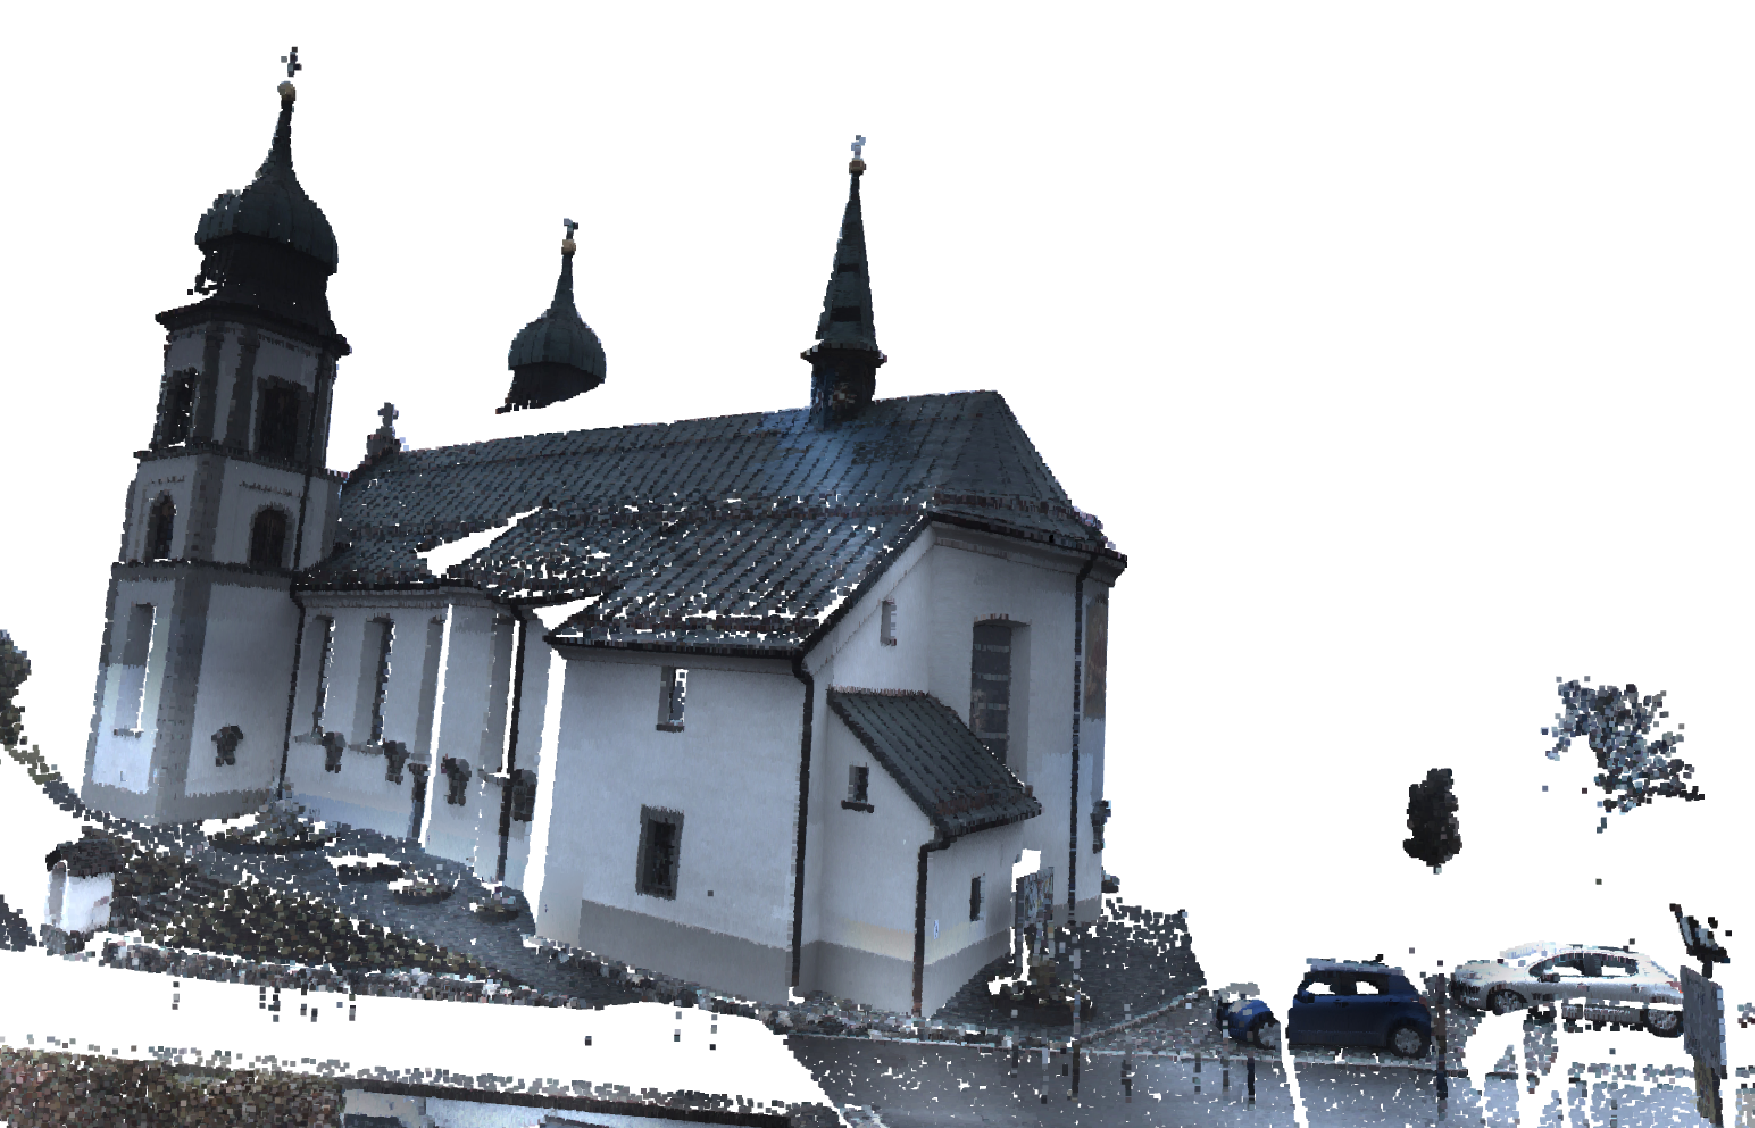
\includegraphics[width=0.33\textwidth, height=0.18\textheight]{images/seg_output/sem3d_seg_output/1_RGB.pdf} &
            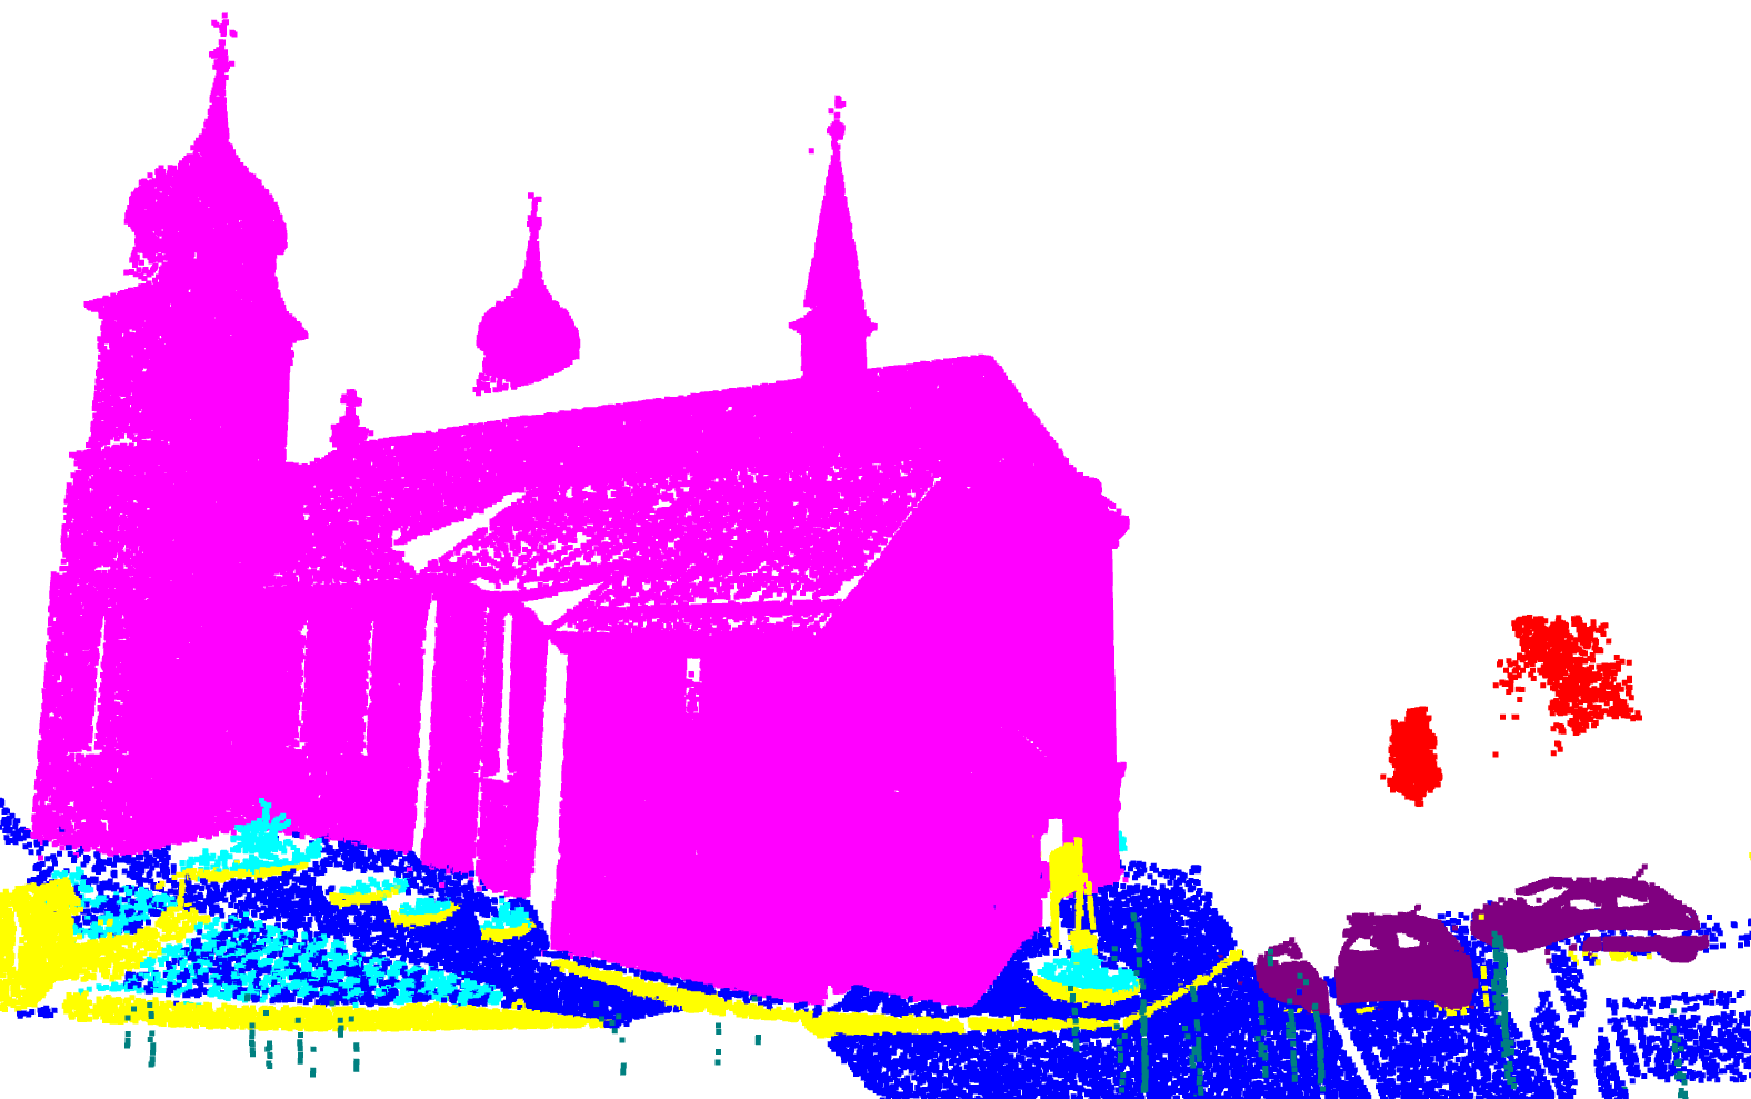
\includegraphics[width=0.33\textwidth, height=0.18\textheight]{images/seg_output/sem3d_seg_output/1_GT.pdf}& 
            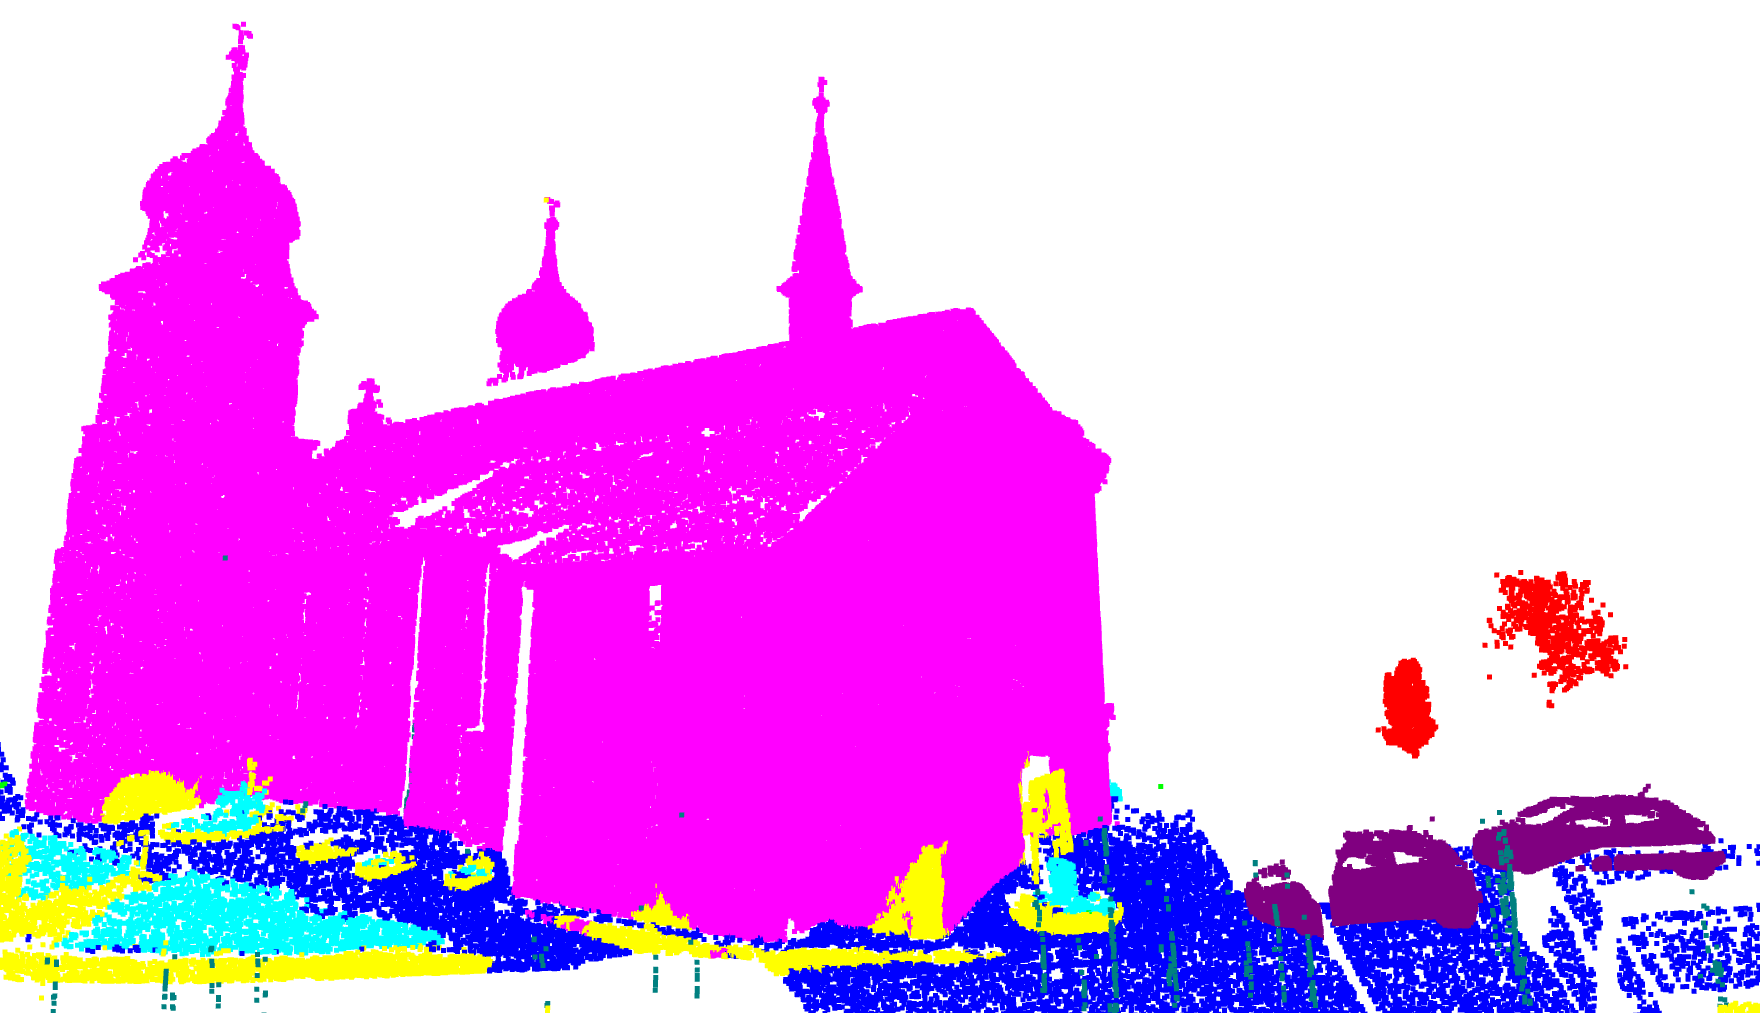
\includegraphics[width=0.33\textwidth, height=0.18\textheight]{images/seg_output/sem3d_seg_output/1_Pred.pdf}\\

            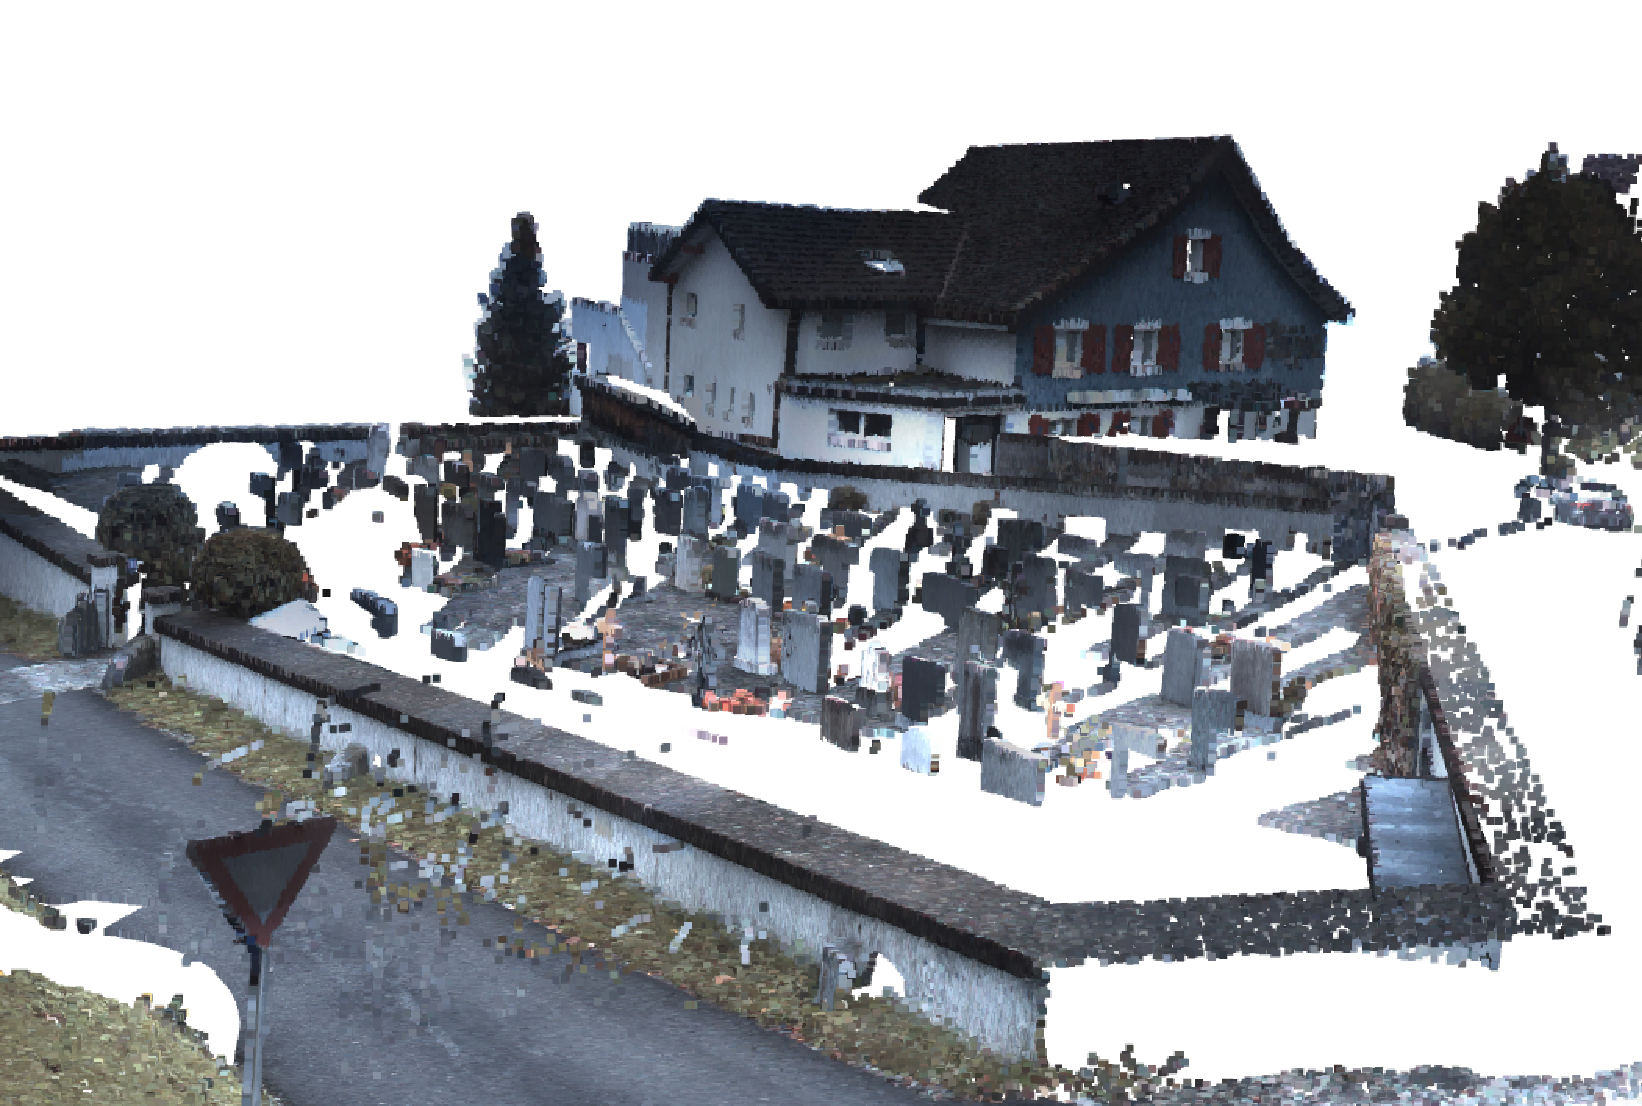
\includegraphics[width=0.33\textwidth, height=0.18\textheight]{images/seg_output/sem3d_seg_output/2_RGB.pdf} &
            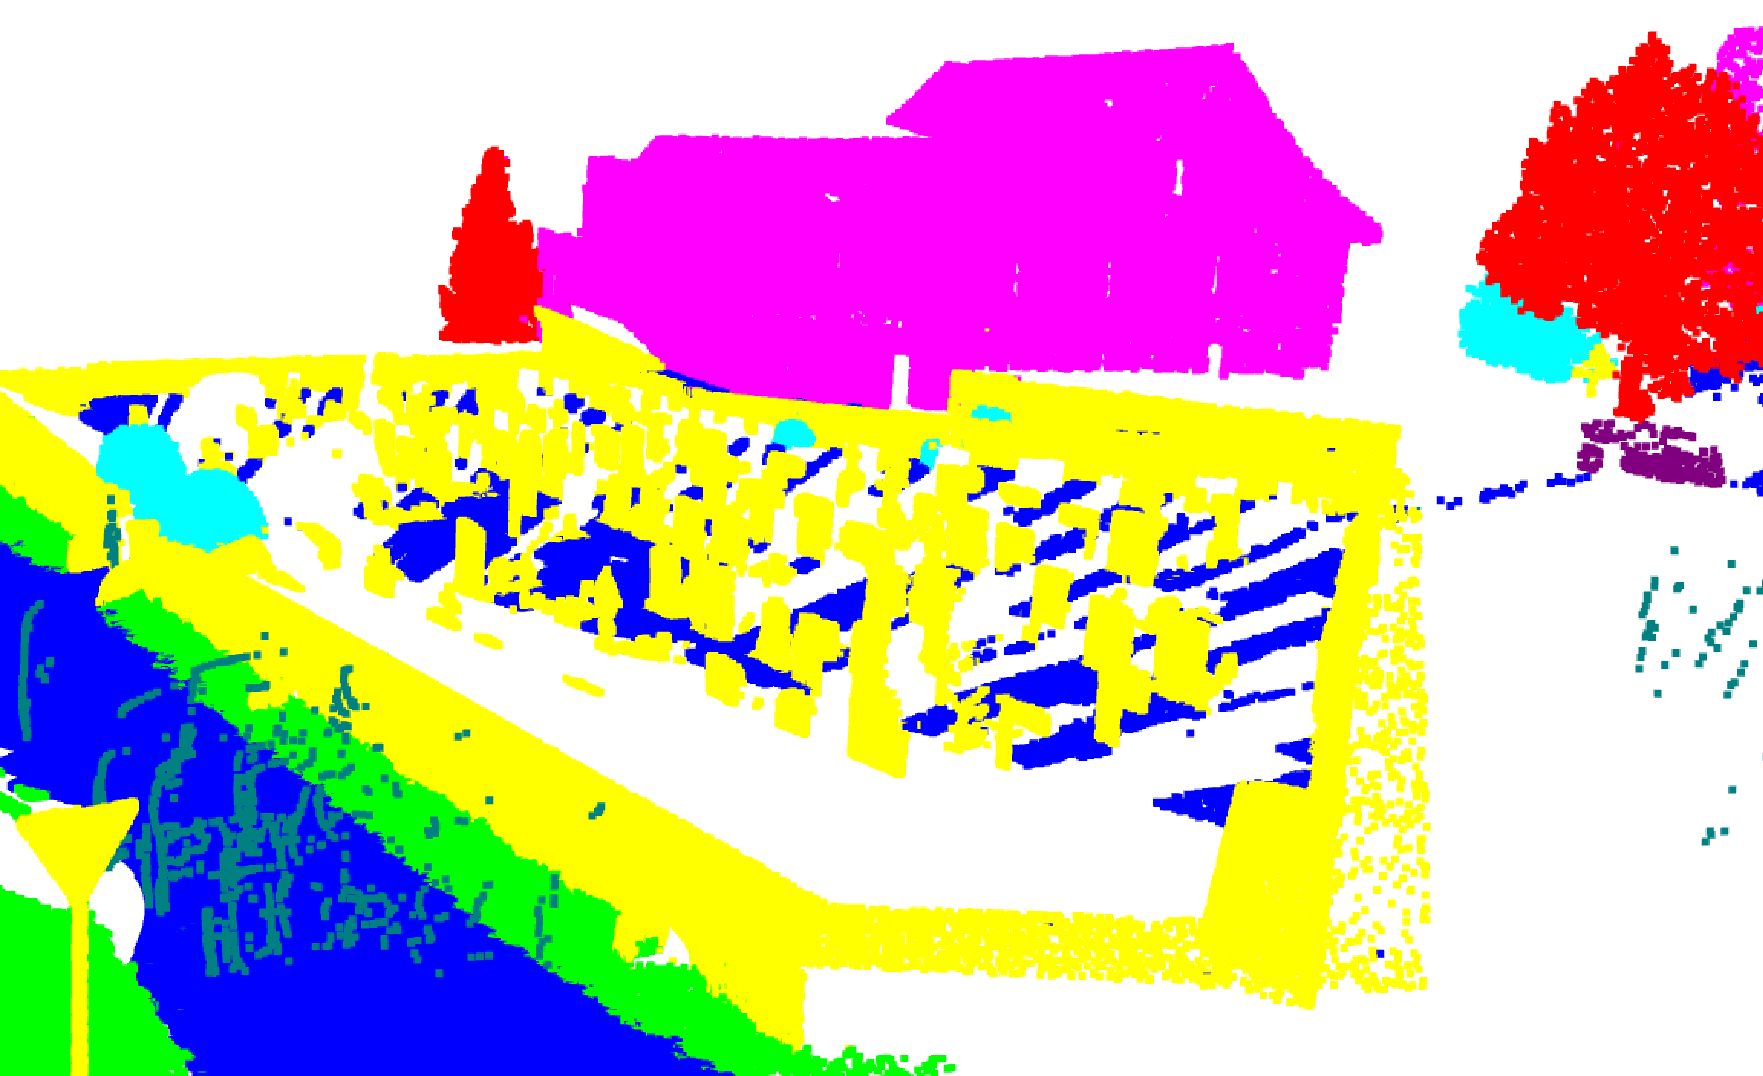
\includegraphics[width=0.33\textwidth, height=0.18\textheight]{images/seg_output/sem3d_seg_output/2_GT.pdf}& 
            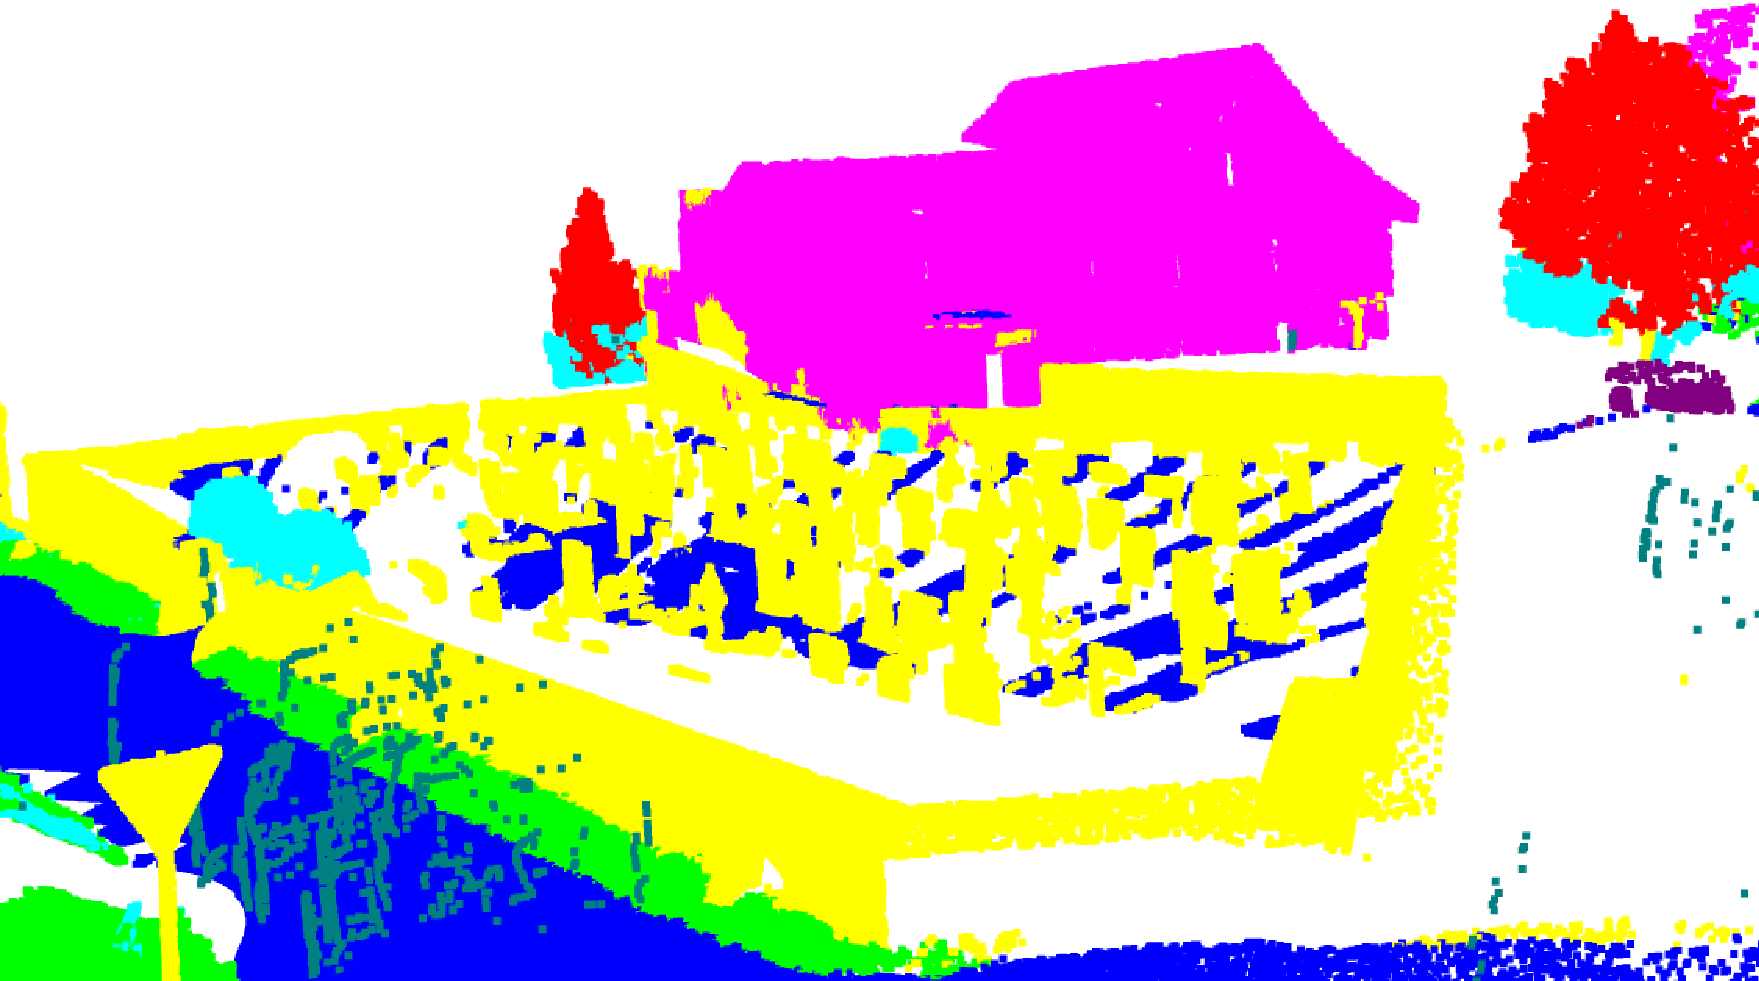
\includegraphics[width=0.33\textwidth, height=0.18\textheight]{images/seg_output/sem3d_seg_output/2_Pred.pdf}\\

            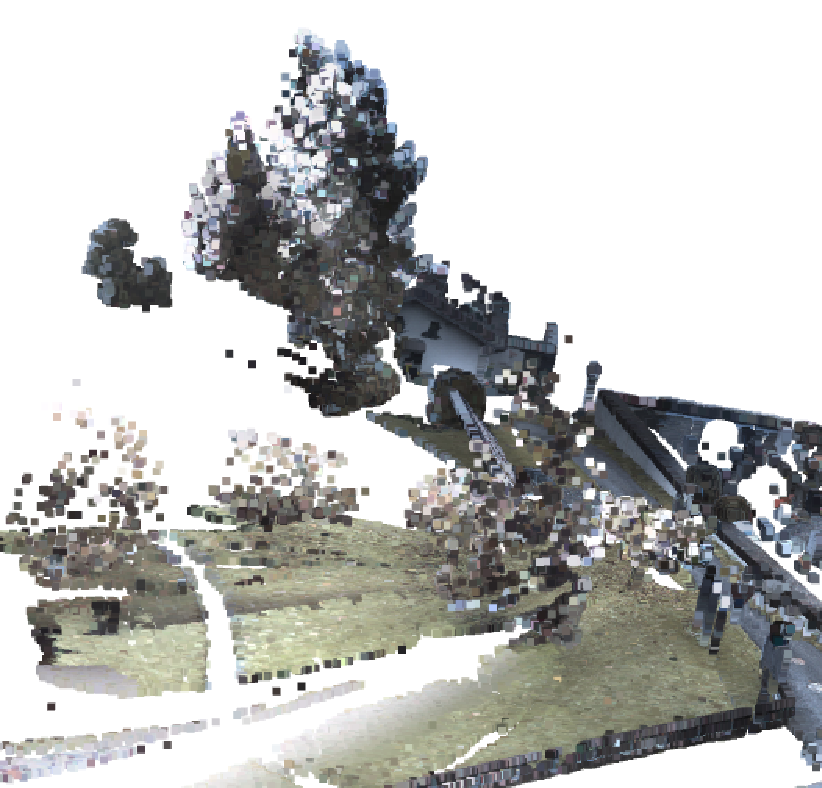
\includegraphics[width=0.33\textwidth, height=0.18\textheight]{images/seg_output/sem3d_seg_output/3_RGB.pdf} &
            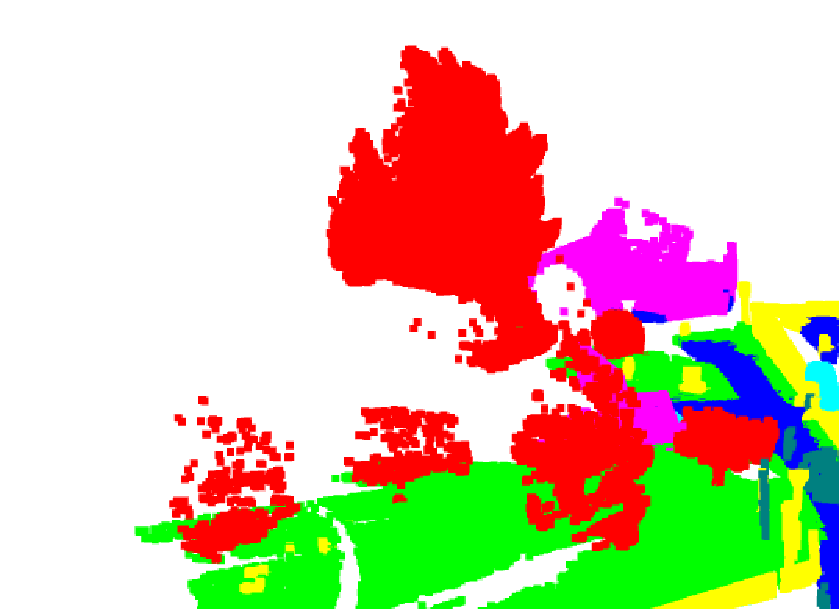
\includegraphics[width=0.33\textwidth, height=0.18\textheight]{images/seg_output/sem3d_seg_output/3_GT.pdf}& 
            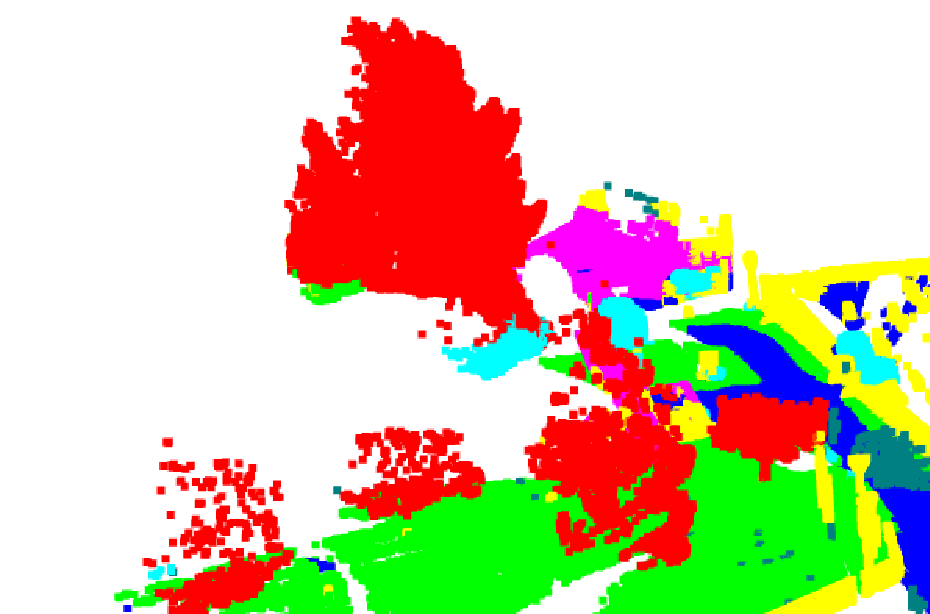
\includegraphics[width=0.33\textwidth, height=0.18\textheight]{images/seg_output/sem3d_seg_output/3_Pred.pdf}\\
        \end{tabular}
        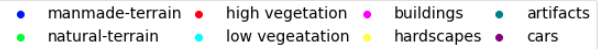
\includegraphics[scale=0.45]{images/legend.png}
        \caption{Image representing the predictions (last column) from Deep Ensemble with an ensemble size of 15 on Semantic3D dataset.
         The first column depict input point cloud and second column represent the ground truth.}
        \label{fig:deepensemble_vis_sem3d}
    \end{figure*}

    % %%%%%% Segmentation output here %%%%%%
    
    % %%%%%% Ensembles output here %%%%%%
    \begin{figure*}[h!]
        \begin{tabular}{cccc}
            Ensmeble Size-1 & Ensemble Size-5 & Ensemble Size-10 \\
            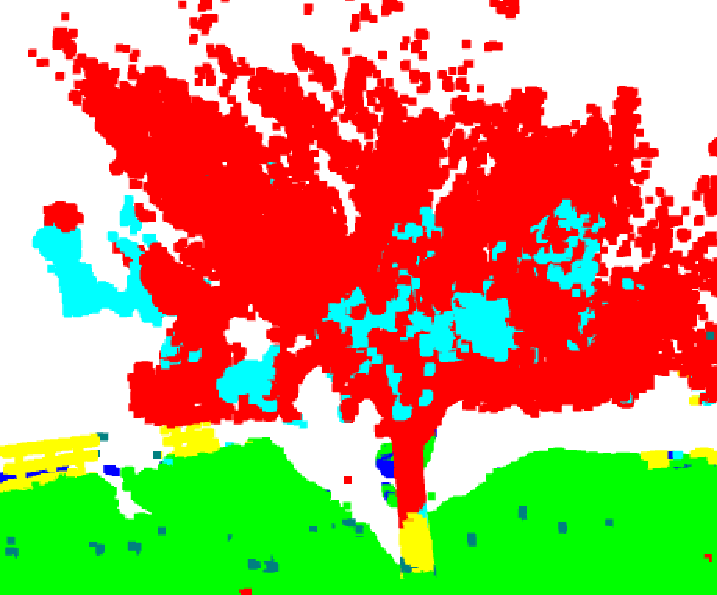
\includegraphics[width=0.30\textwidth, height=0.15\textheight]{images/seg_output/deep_ensembles/1_1.pdf} &
            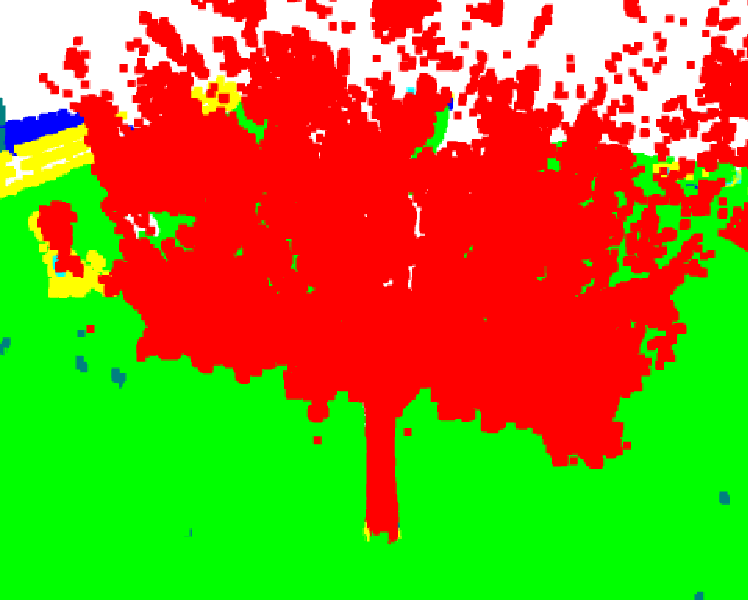
\includegraphics[width=0.30\textwidth, height=0.15\textheight]{images/seg_output/deep_ensembles/1_5.pdf}& 
            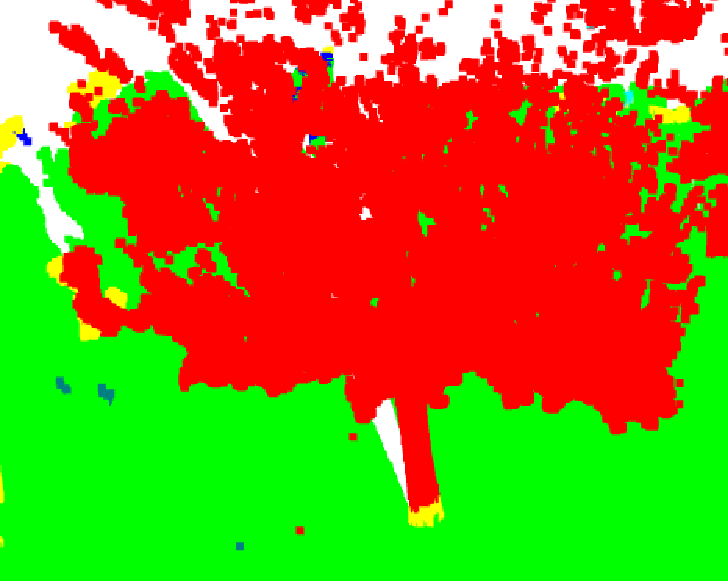
\includegraphics[width=0.30\textwidth, height=0.15\textheight]{images/seg_output/deep_ensembles/1_10.pdf}\\

            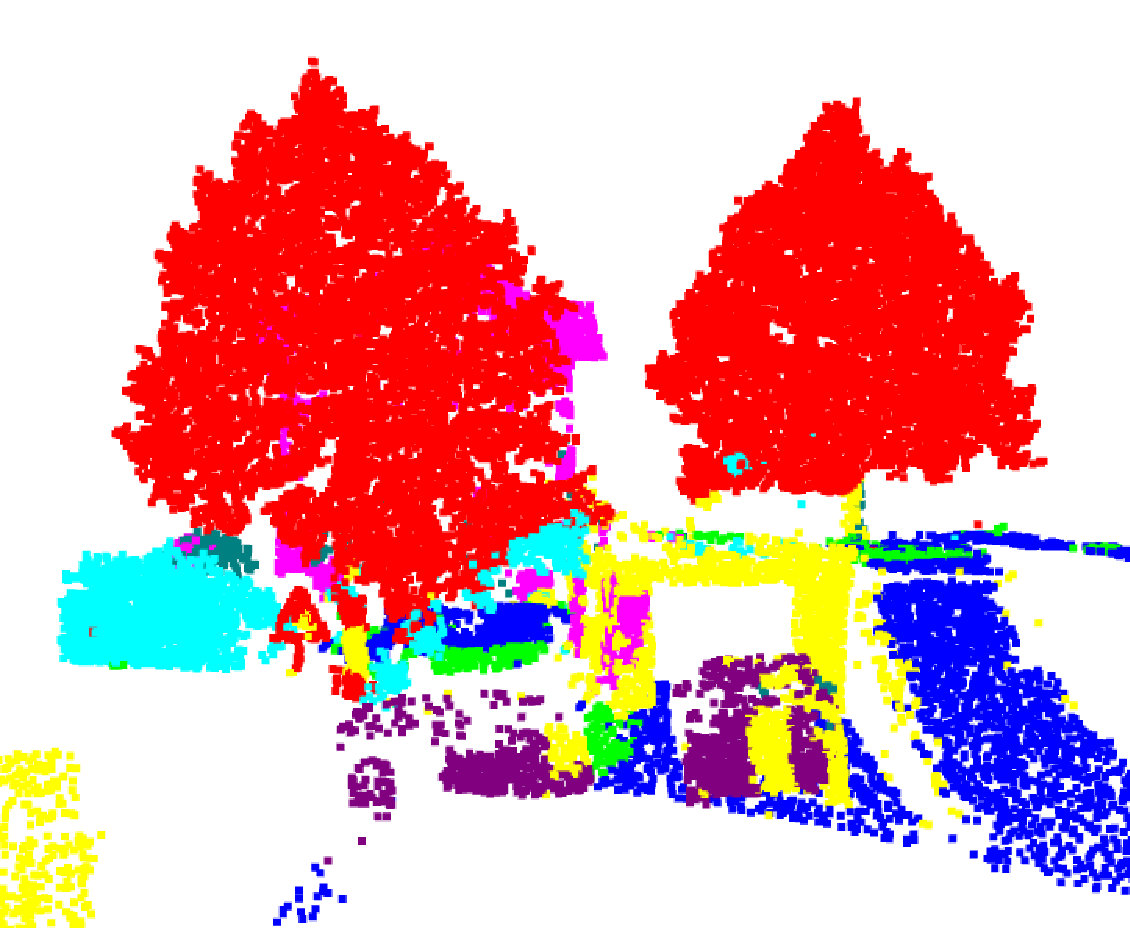
\includegraphics[width=0.30\textwidth, height=0.15\textheight]{images/seg_output/deep_ensembles/2_1.pdf} &
            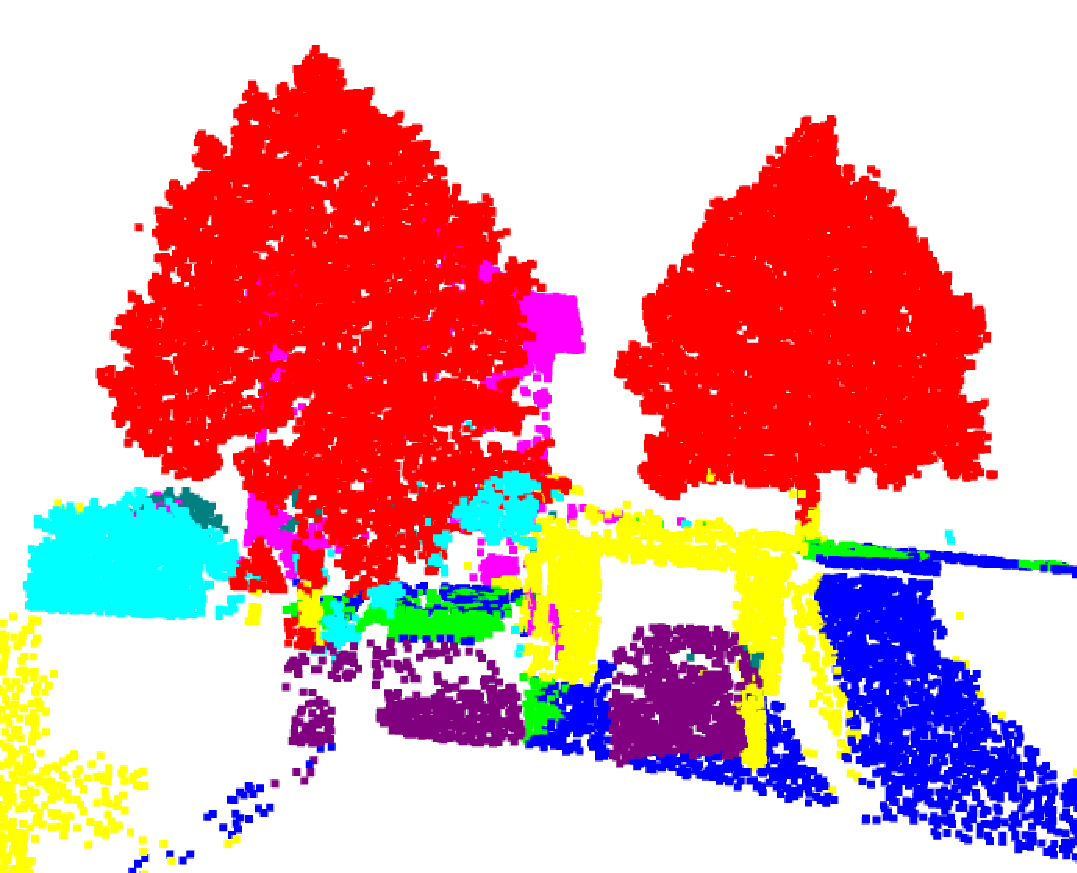
\includegraphics[width=0.30\textwidth, height=0.15\textheight]{images/seg_output/deep_ensembles/2_5.pdf}& 
            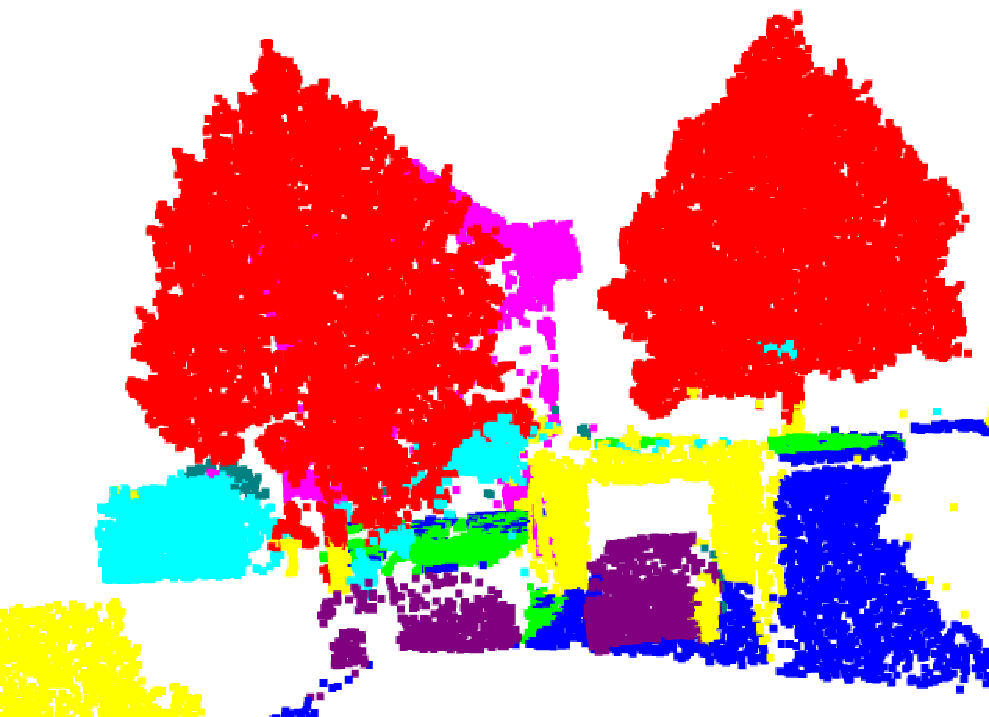
\includegraphics[width=0.30\textwidth, height=0.15\textheight]{images/seg_output/deep_ensembles/2_10.pdf}\\
        \end{tabular}
        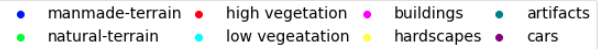
\includegraphics[scale=0.45]{images/legend.png}
        \caption{Performance improvements of Deep Ensembles on Semantic3D dataset with each column representing the ensemble size of 1, 5 and 10 respectively.}
        \label{fig:deepensemble_improv}
    \end{figure*}
    From Table~\ref{tab:ensemble_eval}, we infer that classes ``Low vegetation'' and ``Hardscapes'' have lower per-class IoU scores, this is because these classes are underrepresented in the dataset.
    From Table~\ref{tab:ensemble_eval}, we also infer that the Deep Ensembles improve the model's overall performance in terms of meanIoU and Accuracy.
    With an ensemble size of 10, we observe a 2\% increment on meanIoU.
    An increase in ensemble size also results in an improvement in per-class IoU performance.
    Figure~\ref{fig:deepensemble_improv} depicts the improvement in model classifications with the increase in ensemble size.
    From Figure~\ref{fig:deepensemble_vis_sem3d}, we also observe the misclassifications along the edges of the church, trees and ground.
    The possible explanation for these misclassifications is ambiguity in the feature vector of RandLA-Net. For example, a feature vector for the point along the lower edge of the church contains the part of ground points as the feature vector.
%%%%%%%%%%%%%%%%%%%%%%%%%%%%%%%%%%%%%%%%%%%%%%%%%%%%%%%%%%%%%%%%%%%%%%%%%%%%%%%
    \section{Flipout-Semantic3D}
    In this experiment, we trained a Flipout version of RandLA-Net as described in Section~\ref{sec:flipout_setup} over the Semantic3D dataset.
    Like Deep Ensembles, we performed 20 forward passes over the Flipout-versioned RandLA-Net and averaged the predictions to obtain final predictions.
    Table~\ref{tab:flipout_eval} describes the performance of Flipout-versioned RandLA-Net using meanIoU, per-class IoU and Accuracy.
    Figure~\ref{fig:flipout_vis_sem3d} depicts the predictions of the Flipout-versioned RandLA-Net visually.
    \begin{table}[h!]
        \resizebox{\textwidth}{!}{%
        \begin{tabular}{c|c|cccccccc|c}
        %\textbf{\#Ensembles} & \textbf{MeanIOU} & \textbf{Accuracy} & \textbf{Manmadeterrain} & \textbf{Naturalterrain} & \textbf{Highvegetation} & \textbf{Lowvegetation} & \textbf{Buildings} & \textbf{Hardscapes} & \textbf{Scanningartifacts} & \textbf{Cars} \\ \hline
        & & \multicolumn{7}{c}{\textbf{IoU per-class}} & \\ \hline
        \textbf{\#Passes} & \textbf{MeanIoU} & \textbf{C1} & \textbf{C2} & \textbf{C3} & \textbf{C4} & \textbf{C5} & \textbf{C6} & \textbf{C7} & \textbf{C8} & \textbf{Accuracy} \\ \hline
        1& 69.95  & 94.24&80.09&86.16&22.48&88.70&39.41&57.42&91.12&90.71\\
        5& 69.83  & 94.38&80.21&84.10&23.32&87.80&39.68&57.75&91.43&90.43\\
        10& 69.84 & 94.38&80.16&83.90&23.46&87.73&39.75&57.83&91.47&90.40\\
        15& 69.86 & 94.38&80.17&83.80&23.48&87.73&39.82&57.96&91.57&90.40\\
        20& 69.87 & 94.38&80.18&83.80&23.57&87.72&39.84&57.92&91.57&90.40\\
        \end{tabular}%
        }
        \caption{Illustration of performance of Flipout-versioned RandLA-Net on Semantic3D dataset. meanIOU, IOU per-class and overall accuracy are represented here.
        C1 to C8 are the classes of Semantic3D which are Manmade terrain, Natural terrain, High vegetation, Low vegetation, Buildings, Hardscapes, Scanning artifacts, and Cars.}
        \label{tab:flipout_eval}
    \end{table}
    \begin{figure*}[h!]
        \begin{tabular}{ccc}
            Point Cloud & Ground Truth & Prediction-Flipout \\
            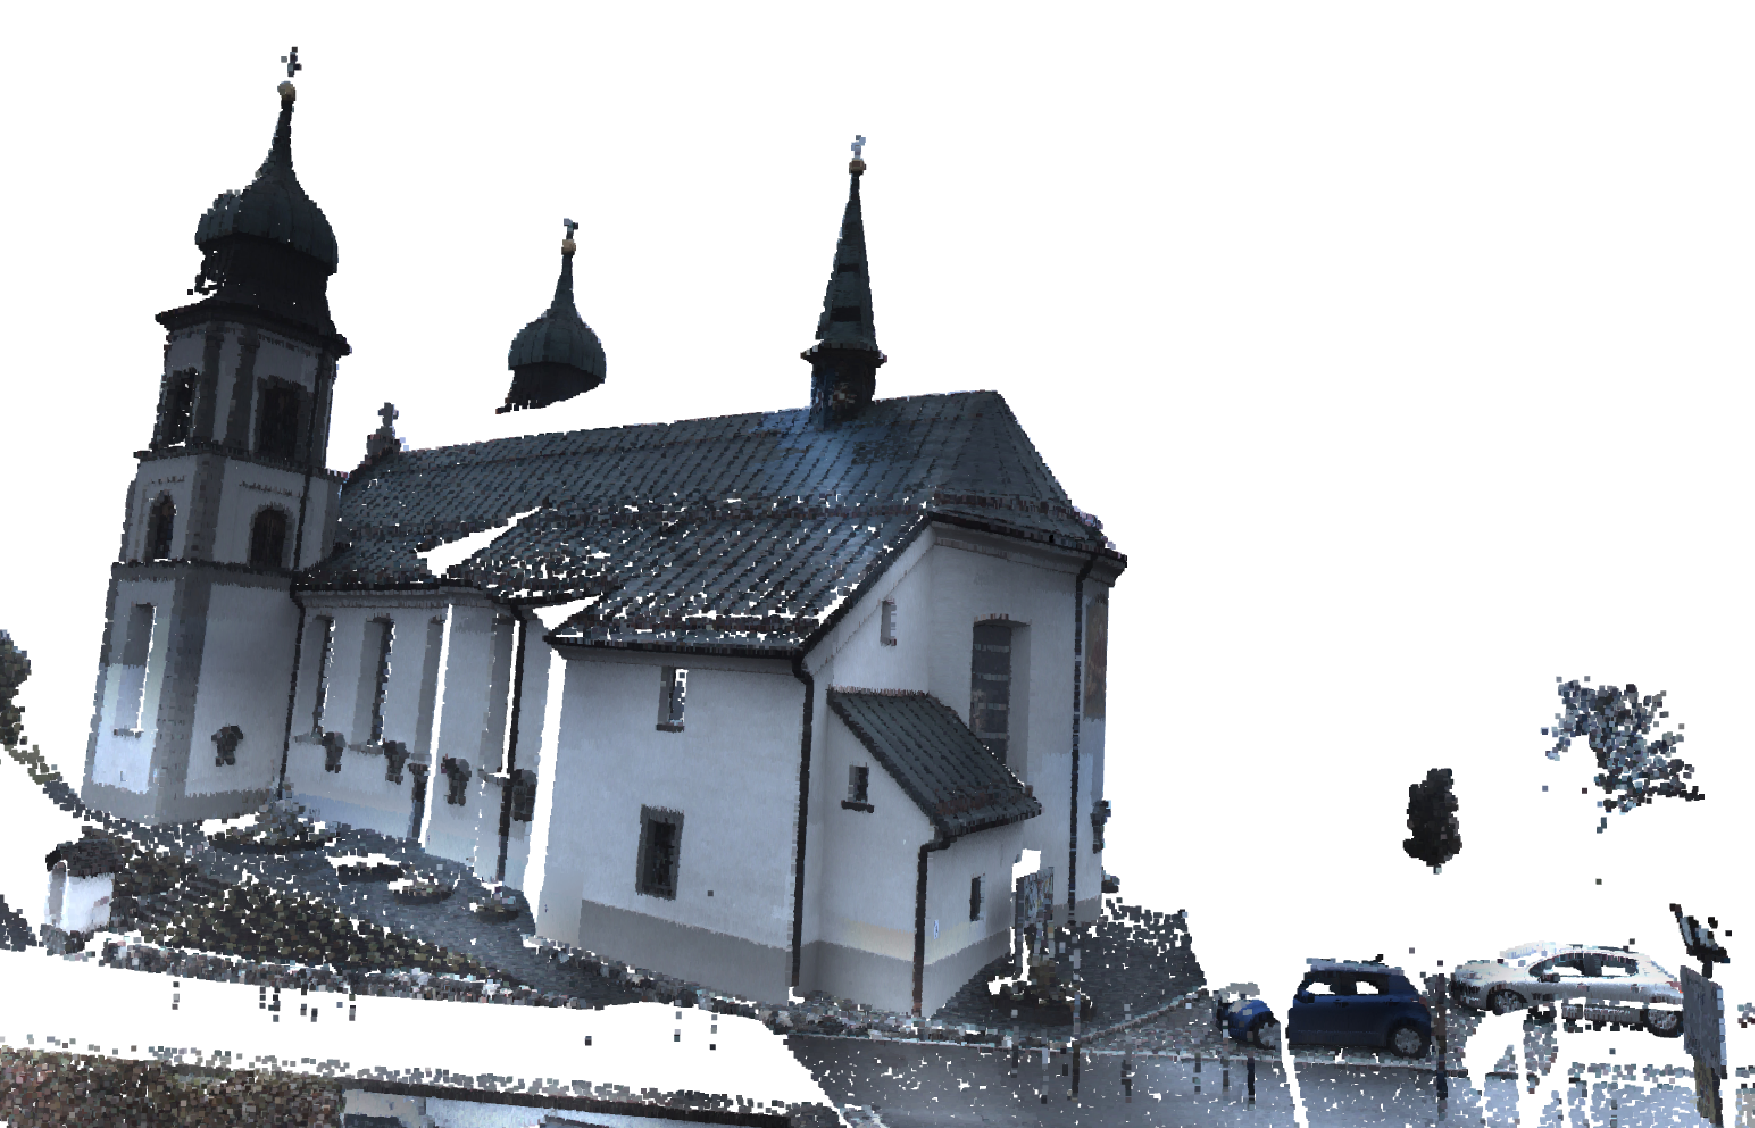
\includegraphics[width=0.33\textwidth, height=0.18\textheight]{images/seg_output/sem3d_seg_output/1_RGB.pdf} &
            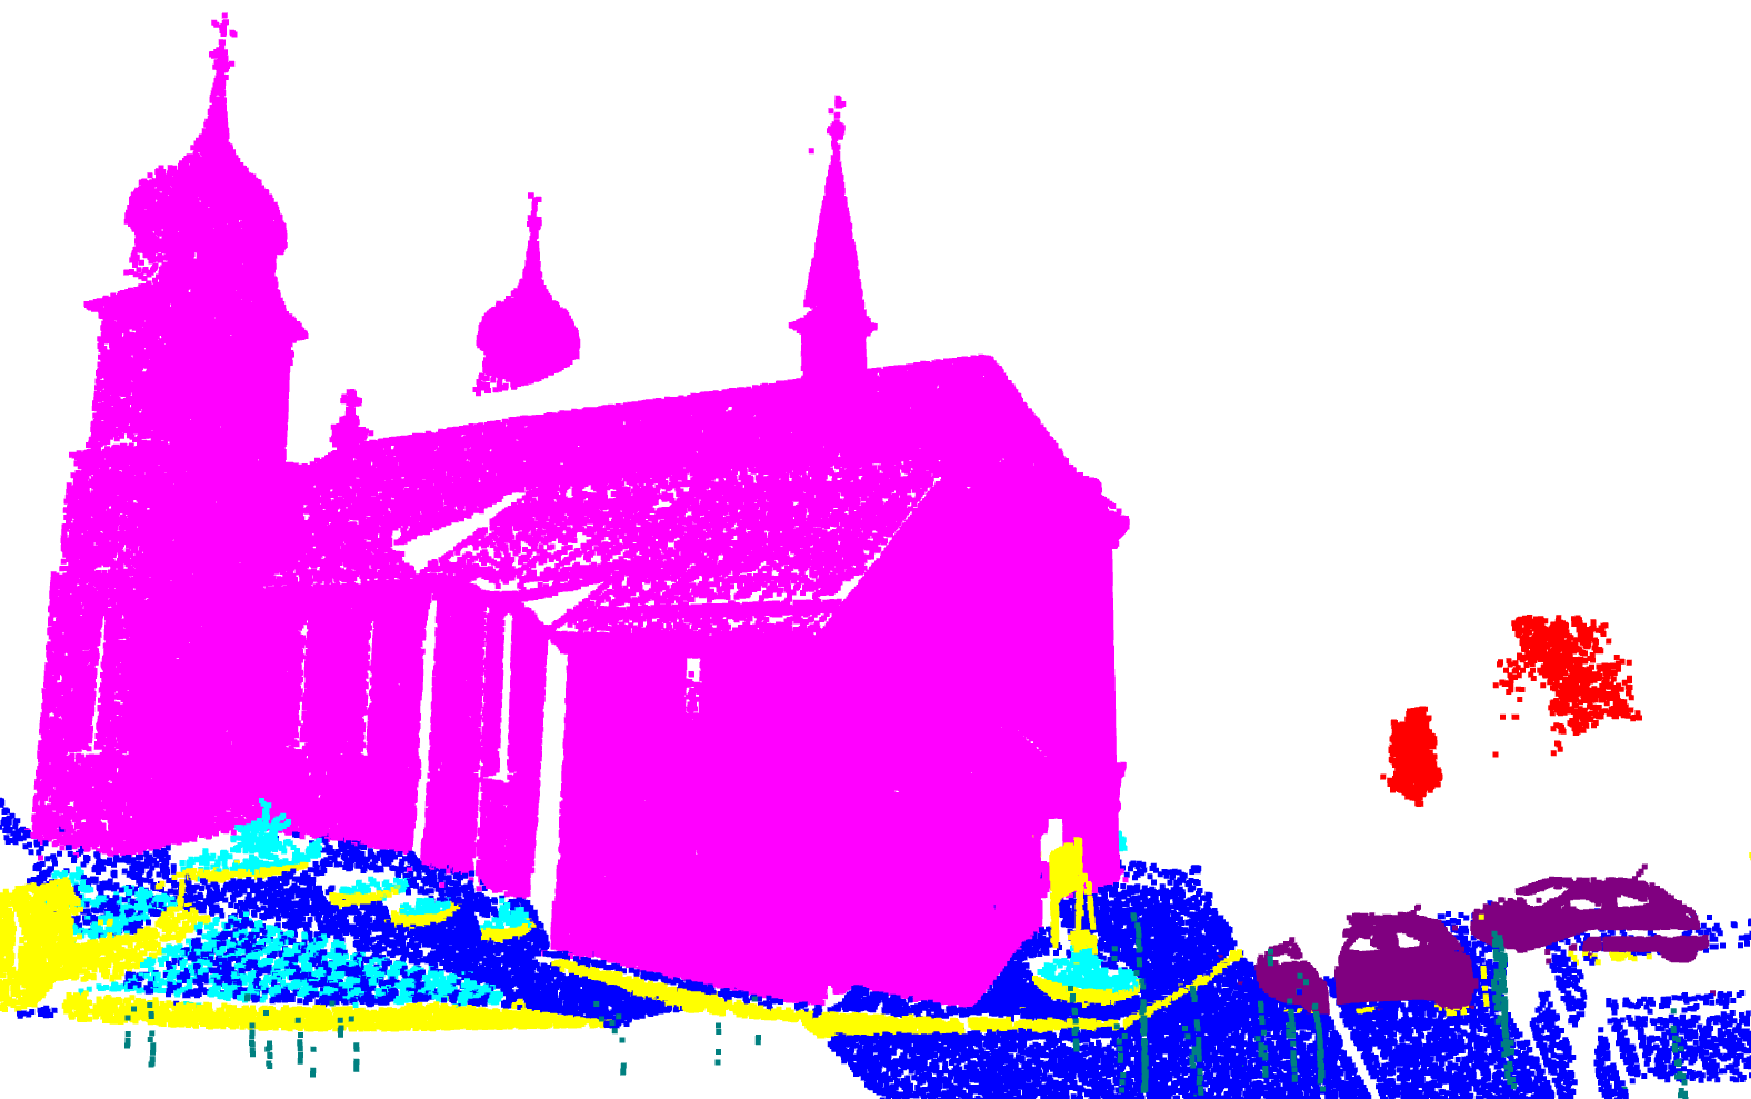
\includegraphics[width=0.33\textwidth, height=0.18\textheight]{images/seg_output/sem3d_seg_output/1_GT.pdf}& 
            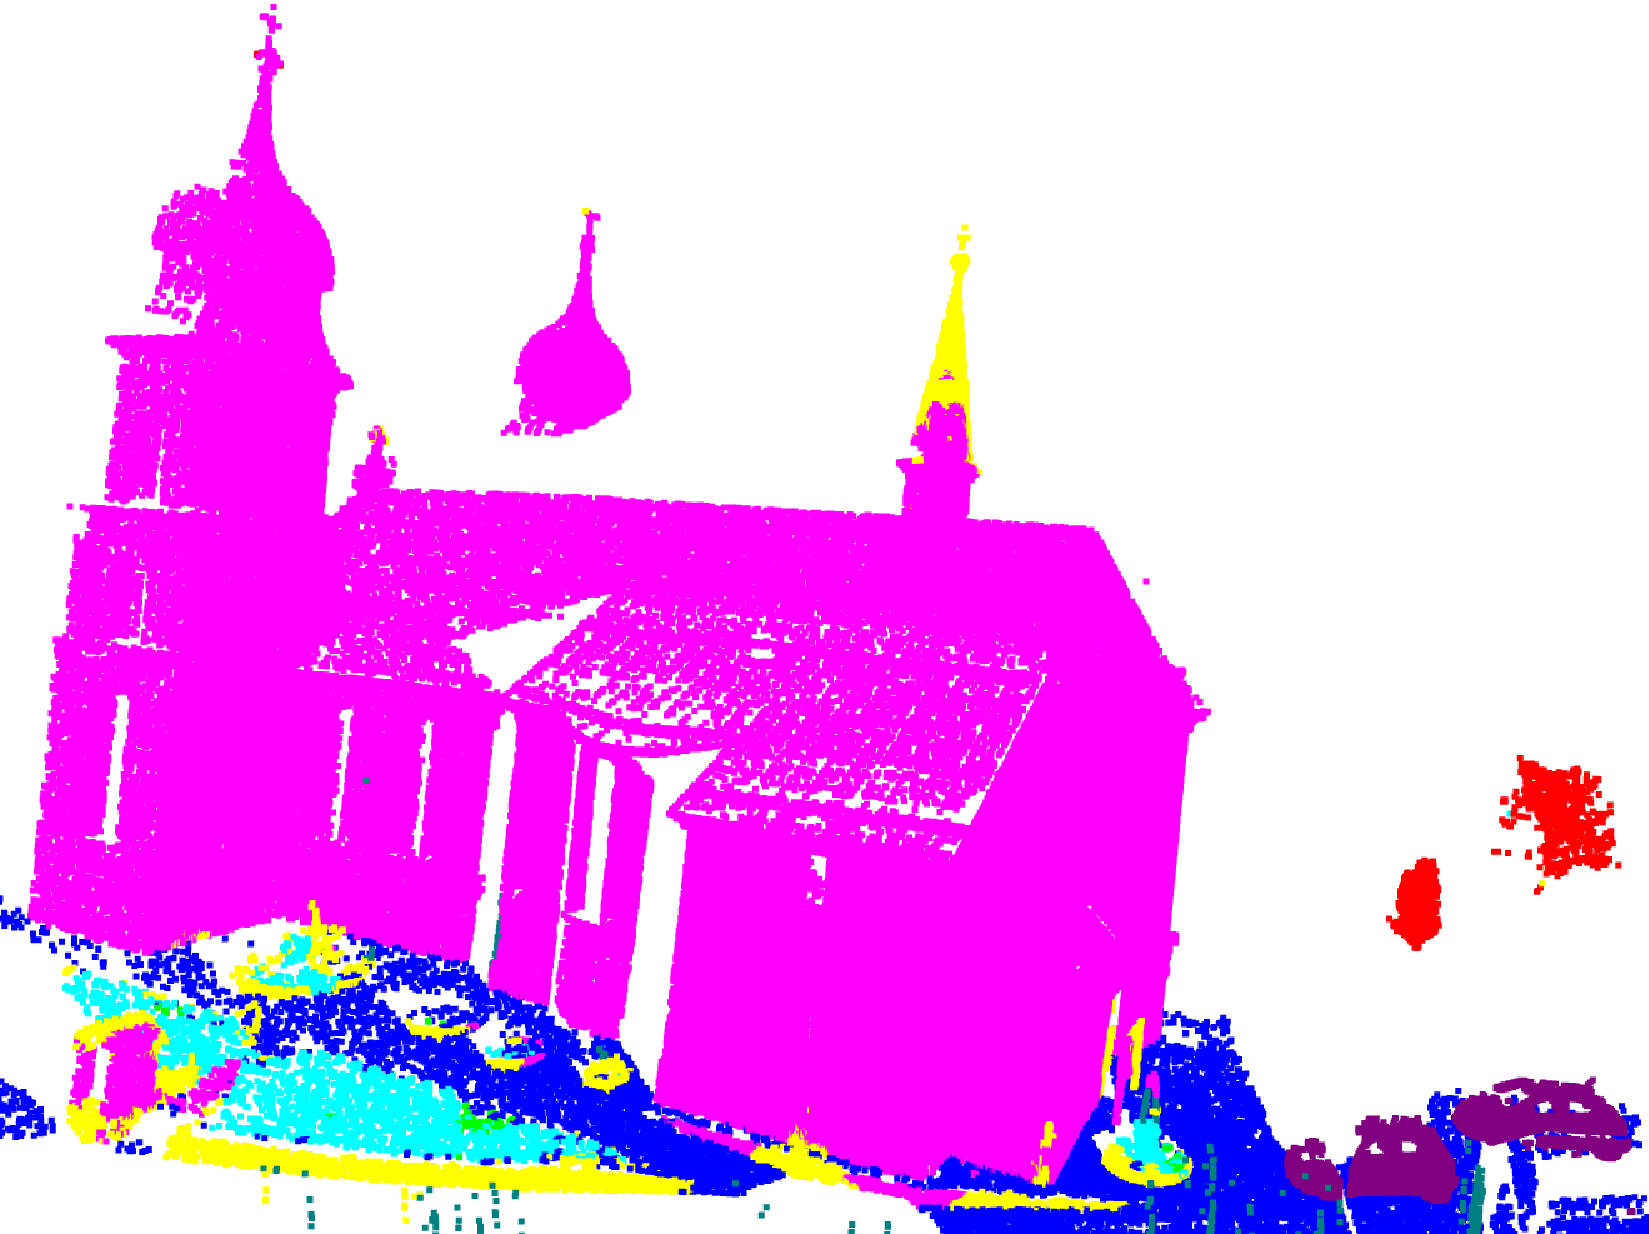
\includegraphics[width=0.33\textwidth, height=0.18\textheight]{images/seg_output/flipout/sem3d_1.pdf}\\

            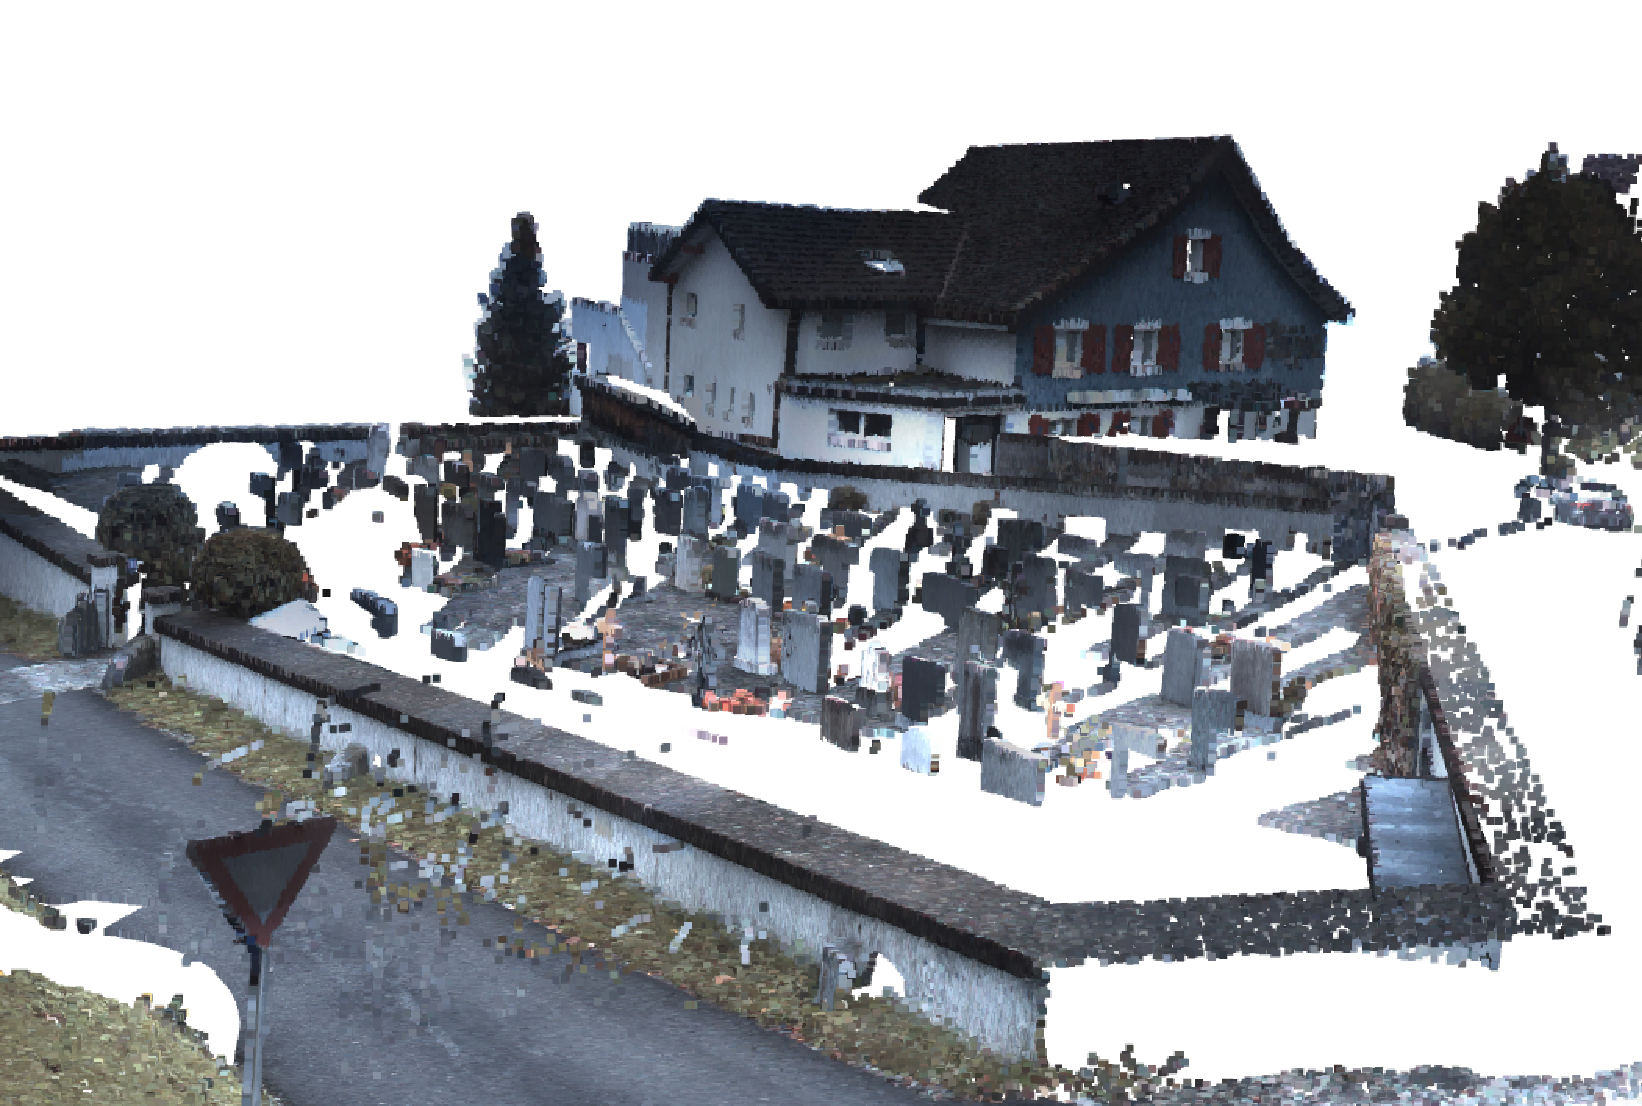
\includegraphics[width=0.33\textwidth, height=0.18\textheight]{images/seg_output/sem3d_seg_output/2_RGB.pdf} &
            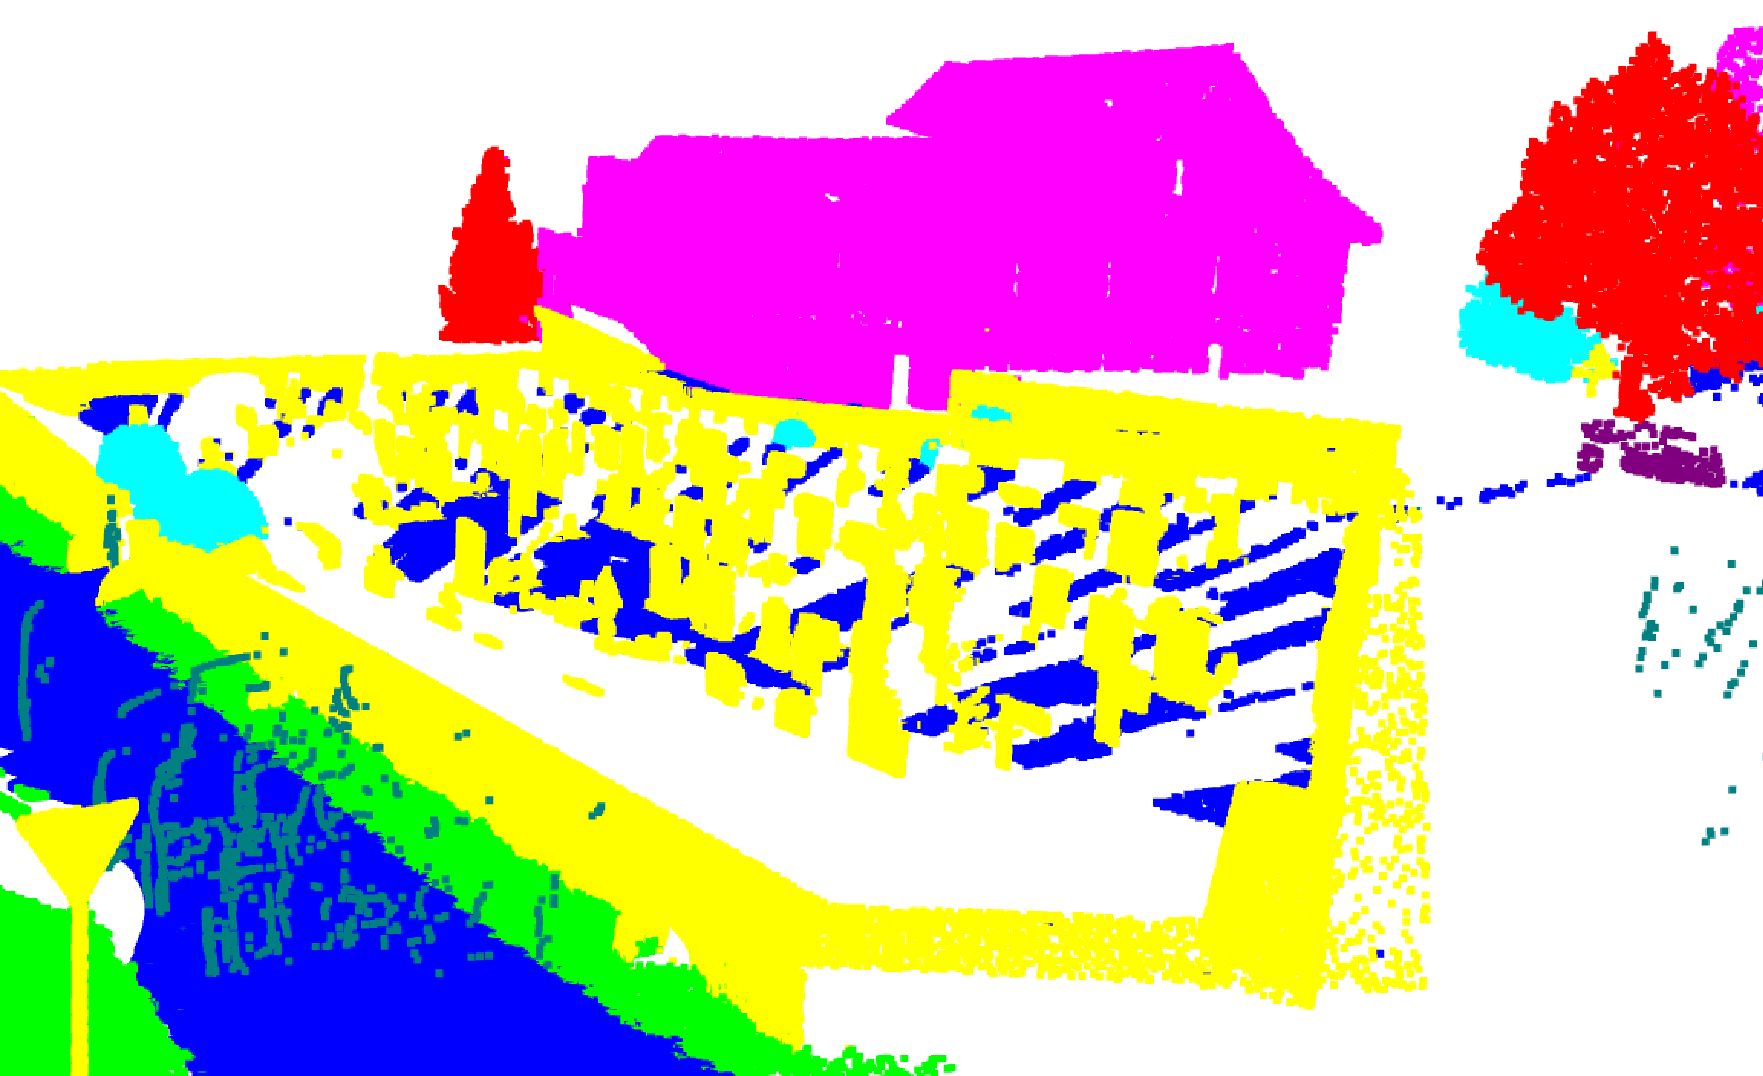
\includegraphics[width=0.33\textwidth, height=0.18\textheight]{images/seg_output/sem3d_seg_output/2_GT.pdf}& 
            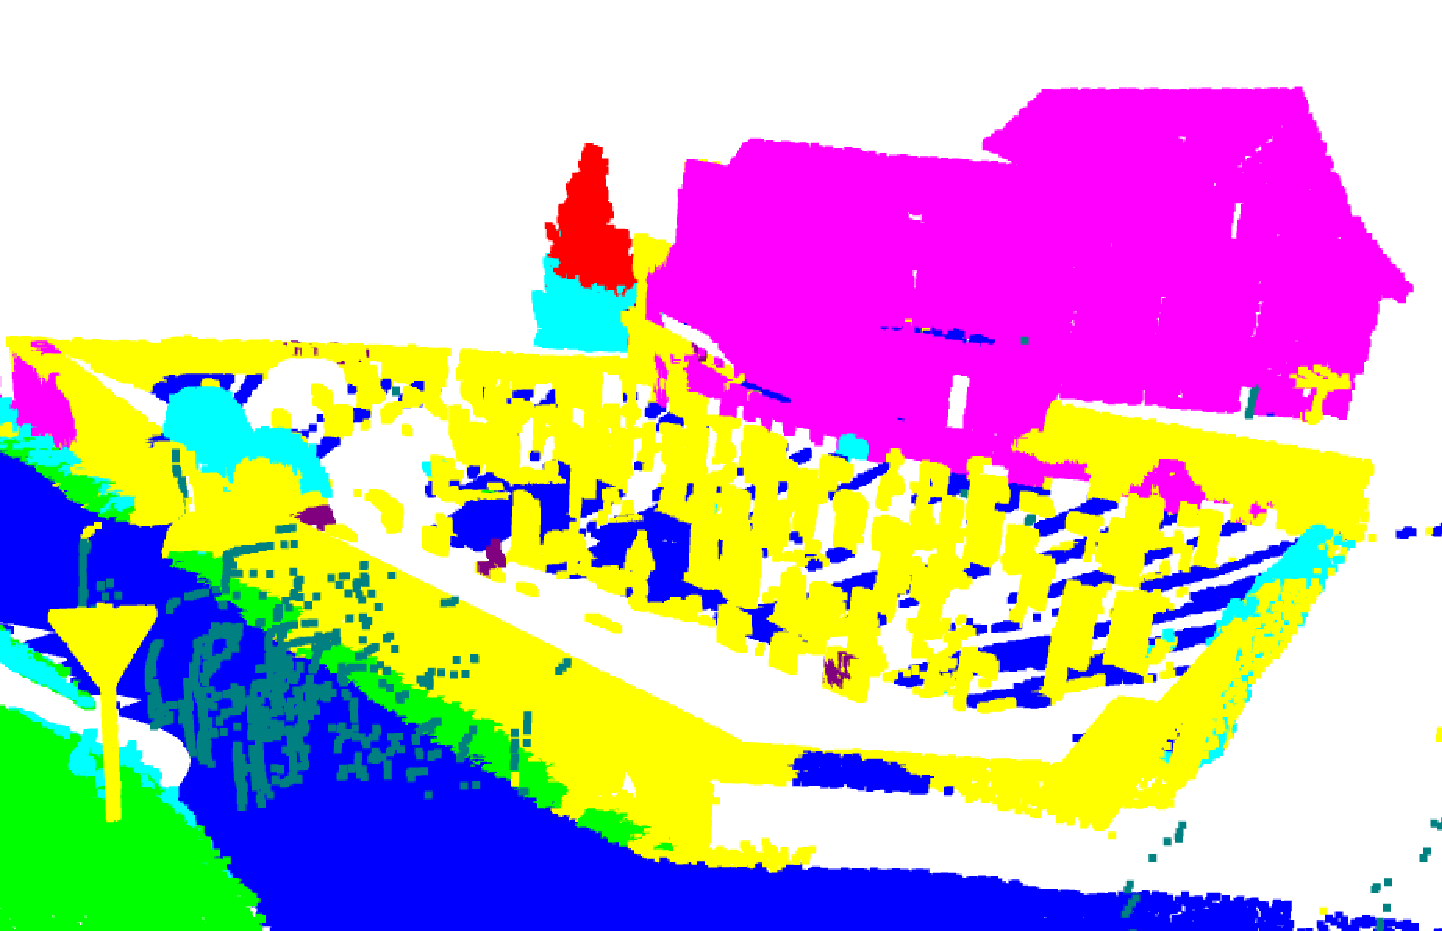
\includegraphics[width=0.33\textwidth, height=0.18\textheight]{images/seg_output/flipout/sem3d_2.pdf}\\

            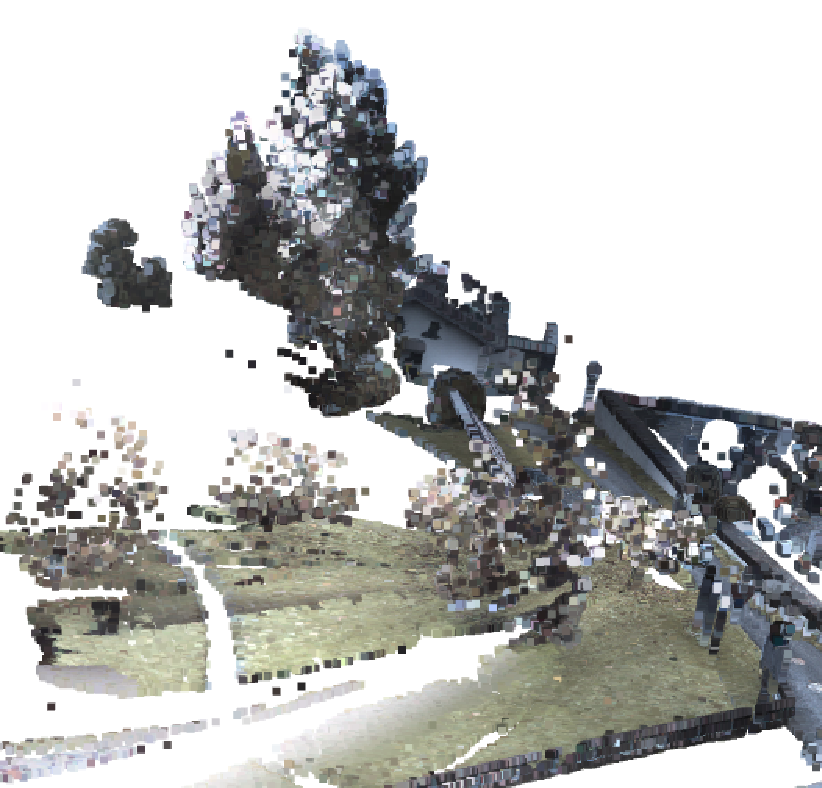
\includegraphics[width=0.33\textwidth, height=0.18\textheight]{images/seg_output/sem3d_seg_output/3_RGB.pdf} &
            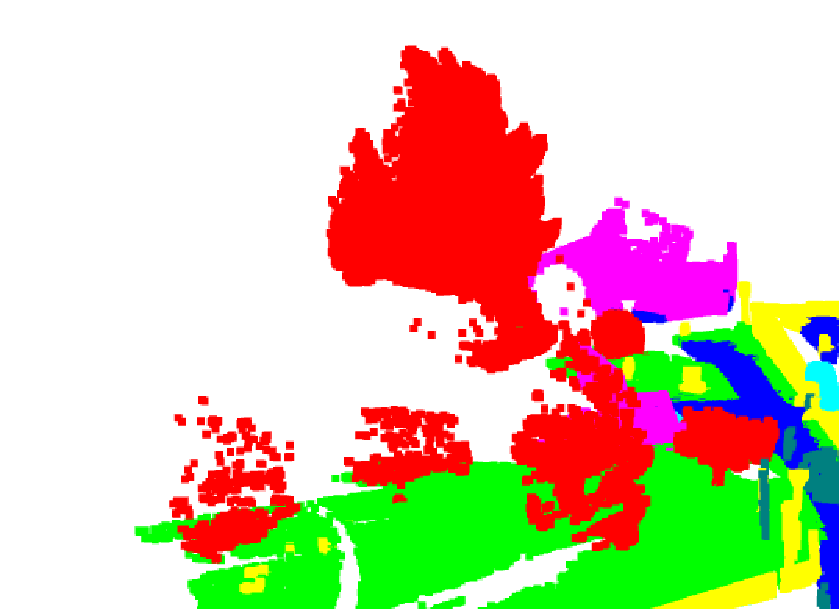
\includegraphics[width=0.33\textwidth, height=0.18\textheight]{images/seg_output/sem3d_seg_output/3_GT.pdf}& 
            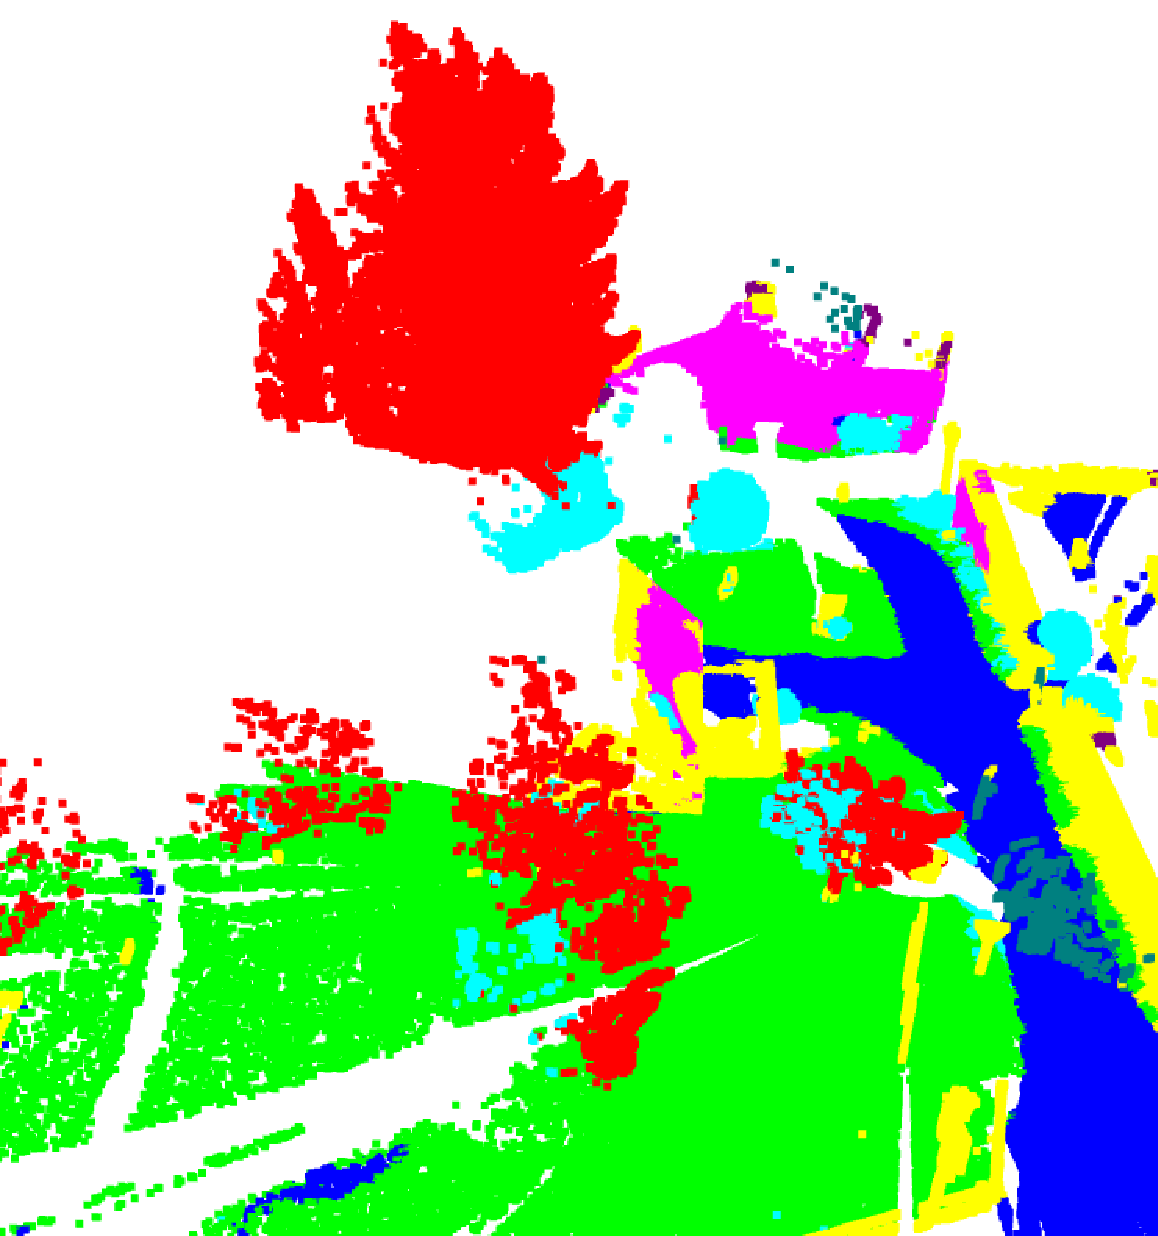
\includegraphics[width=0.33\textwidth, height=0.18\textheight]{images/seg_output/flipout/sem3d_3.pdf}\\
        \end{tabular}
        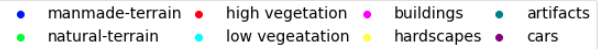
\includegraphics[scale=0.45]{images/legend.png}
        \caption{Image representing the predictions (last column) from Flipout with 15 forward passes on Semantic3D dataset.
        The first column depict input point cloud and second column represent the ground truth.}
        \label{fig:flipout_vis_sem3d}
    \end{figure*}   

    From Table~\ref{tab:flipout_eval}, we infer that the Flipout-versioned RandLA-Net has a similar performance to the original RandLA-Net model proposed in \cite{Hu_2020_CVPR_Randla} and also Deep Ensembles with ensemble size one.
    We also observe a significant improvement in the Hardscapes class represented as C6 in Table~\ref{tab:flipout_eval}.
    There is a decrement in performance of classes Lowvegetation represented as C4 and Scanningartifacts represented as C7 in Table~\ref{tab:flipout_eval}, keeping the overall meanIoU same.
    % \textcolour{red}{Add the images of flipout performance here same as figures in deep ensembles}
    
%%%%%%%%%%%%%%%%%%%%%%%%%%%%%%%%%%%%%%%%%%%%%%%%%%%%%%%%%%%%%%%%%%%%%%%%%%%%%%%
    \section{OOD benchmark - Semantic3D vs S3DIS}
    In the previous section, we studied the performance of the Deep Ensembles and Flipout over the Semantic3D (In-Distribution) dataset.
    In this section, we study the predictions of the RandLA-Net model on the S3DIS (Out-Of-Distribution) dataset using Deep Ensembles and Flipout.
    We also compare the distribution of Maximum Softmax Probability (MSP) and entropy scores for Semantic3D and S3DIS datasets.

    Figure~\ref{fig:de_s3dis_vis} depict the predictions of the RandLA-Net model and Flipout-versioned RandLA-Net.
    We observe that most objects, such as ceilings and bookshelves, are labelled as buildings when using Deep Ensembles.
    We also observe that most point clouds are labelled as hardscapes class when using Flipout-versioned RandLA-Net.
    The classifications on S3DIS datasets are in triangles because of the property of the scanner.
    As discussed in Section~\ref{sec:dataset_s3dis}, data collected from the Matterport scanner is represented as triangular mesh, and then a point cloud is extracted from this mesh.

    \begin{figure*}[h!]
        \centering
        \begin{tabular}{ccc}
            Point Cloud & Deep Ensembles & Flipout \\
            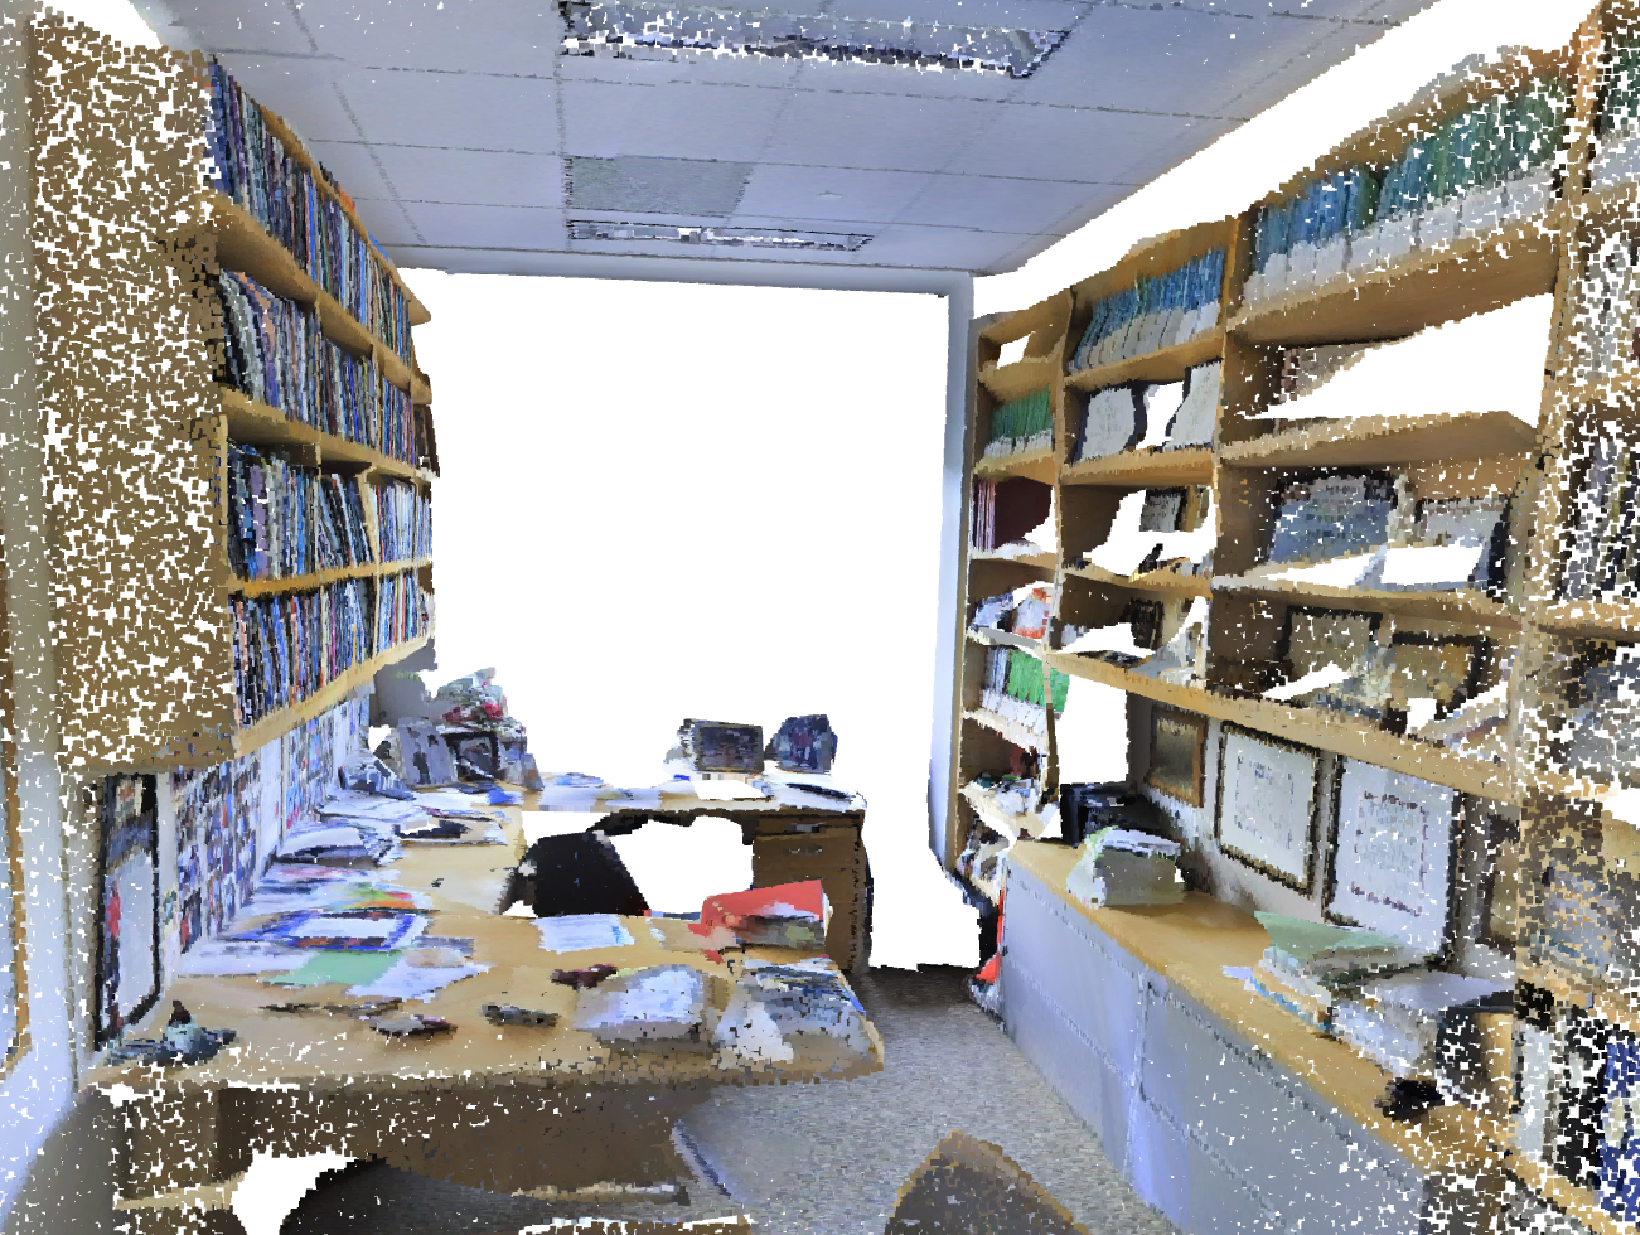
\includegraphics[width=0.33\textwidth, height=0.18\textheight]{images/seg_output/s3dis_DE/S3DIS_1_RGB.pdf} &
            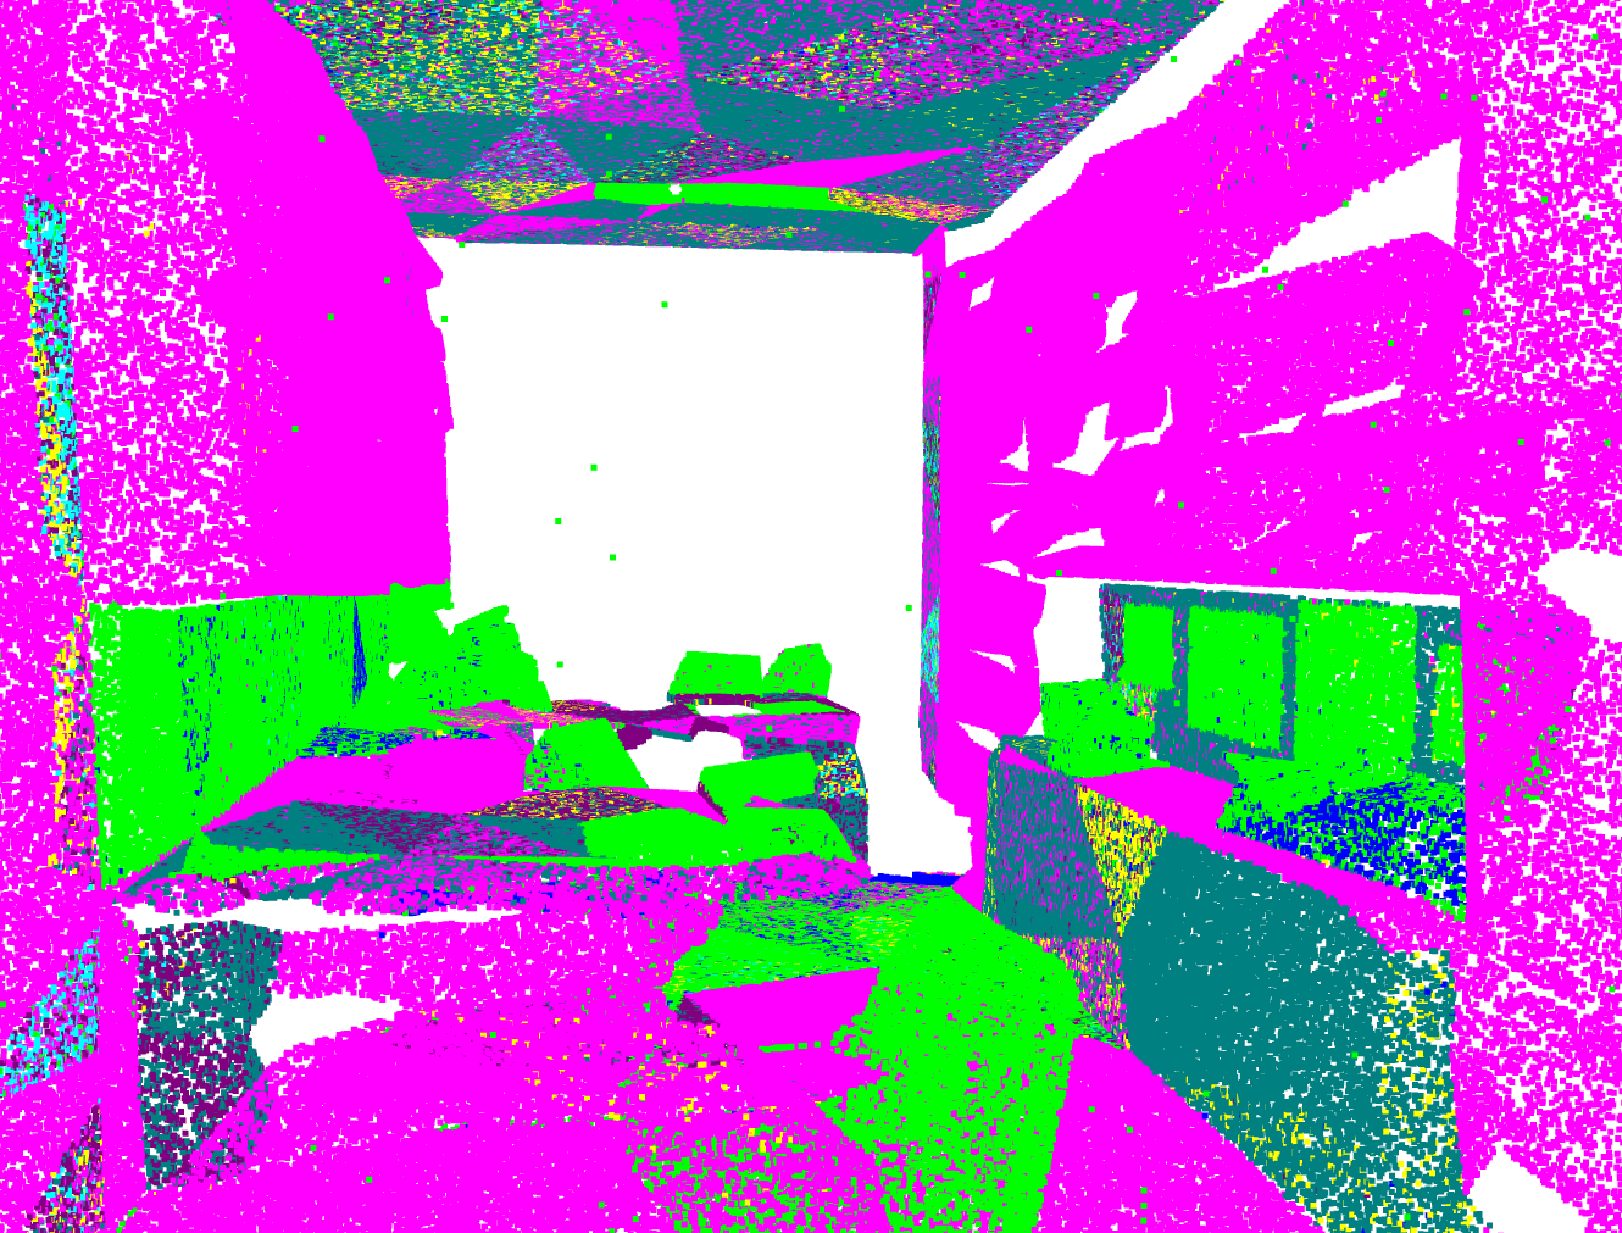
\includegraphics[width=0.33\textwidth, height=0.18\textheight]{images/seg_output/s3dis_DE/S3DIS_1_Pred.pdf} &
            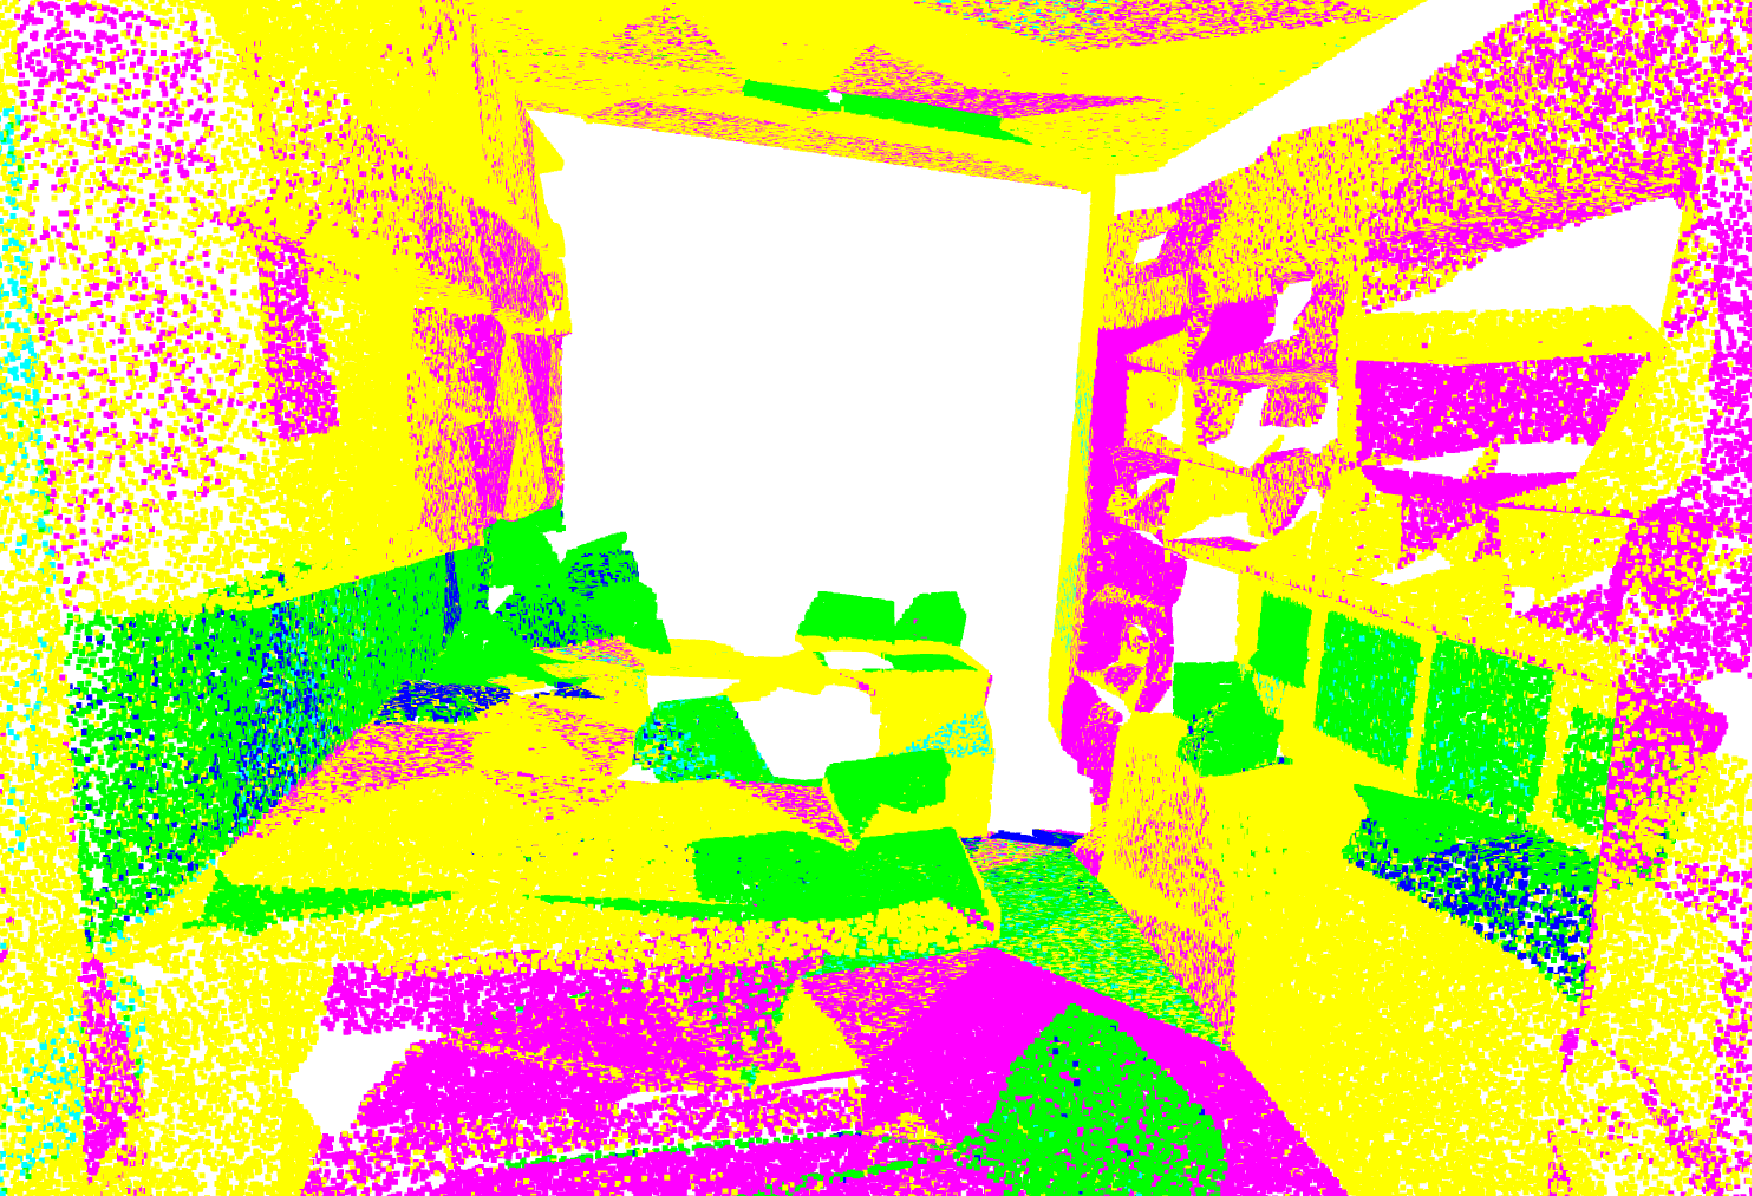
\includegraphics[width=0.33\textwidth, height=0.18\textheight]{images/seg_output/s3dis_DE/office_3.pdf} \\

            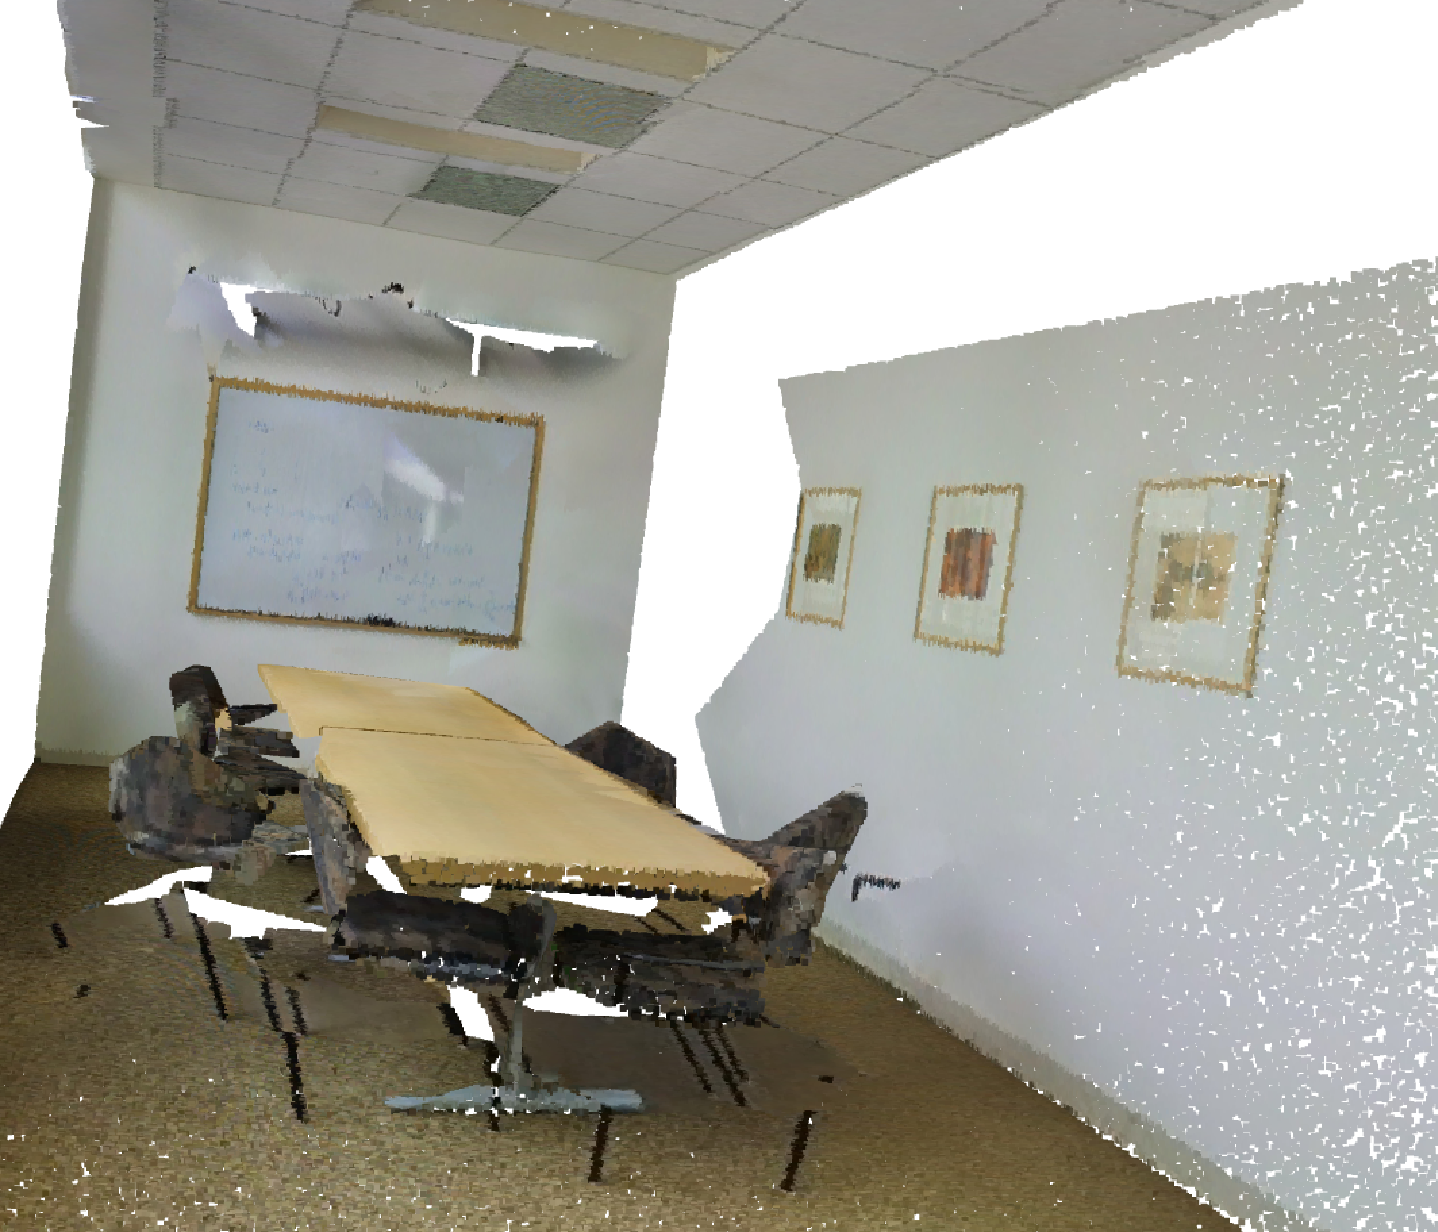
\includegraphics[width=0.33\textwidth, height=0.18\textheight]{images/seg_output/s3dis_DE/S3DIS_2_RGB.pdf} &
            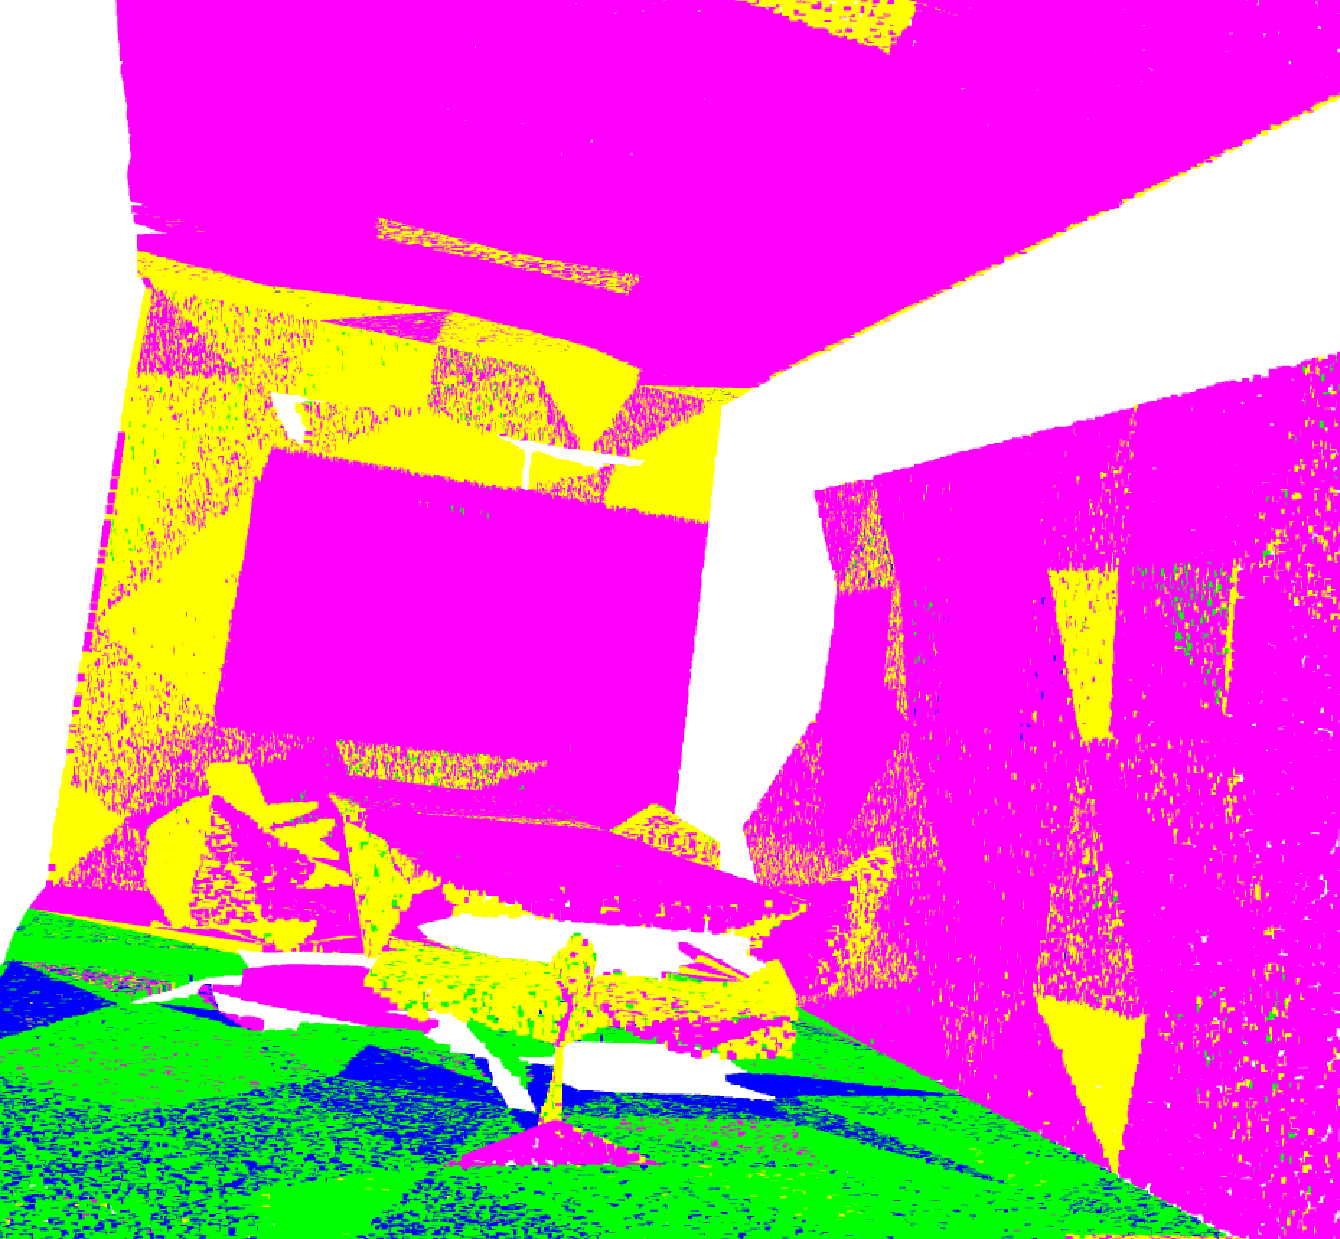
\includegraphics[width=0.33\textwidth, height=0.18\textheight]{images/seg_output/s3dis_DE/S3DIS_2_Pred.pdf}&
            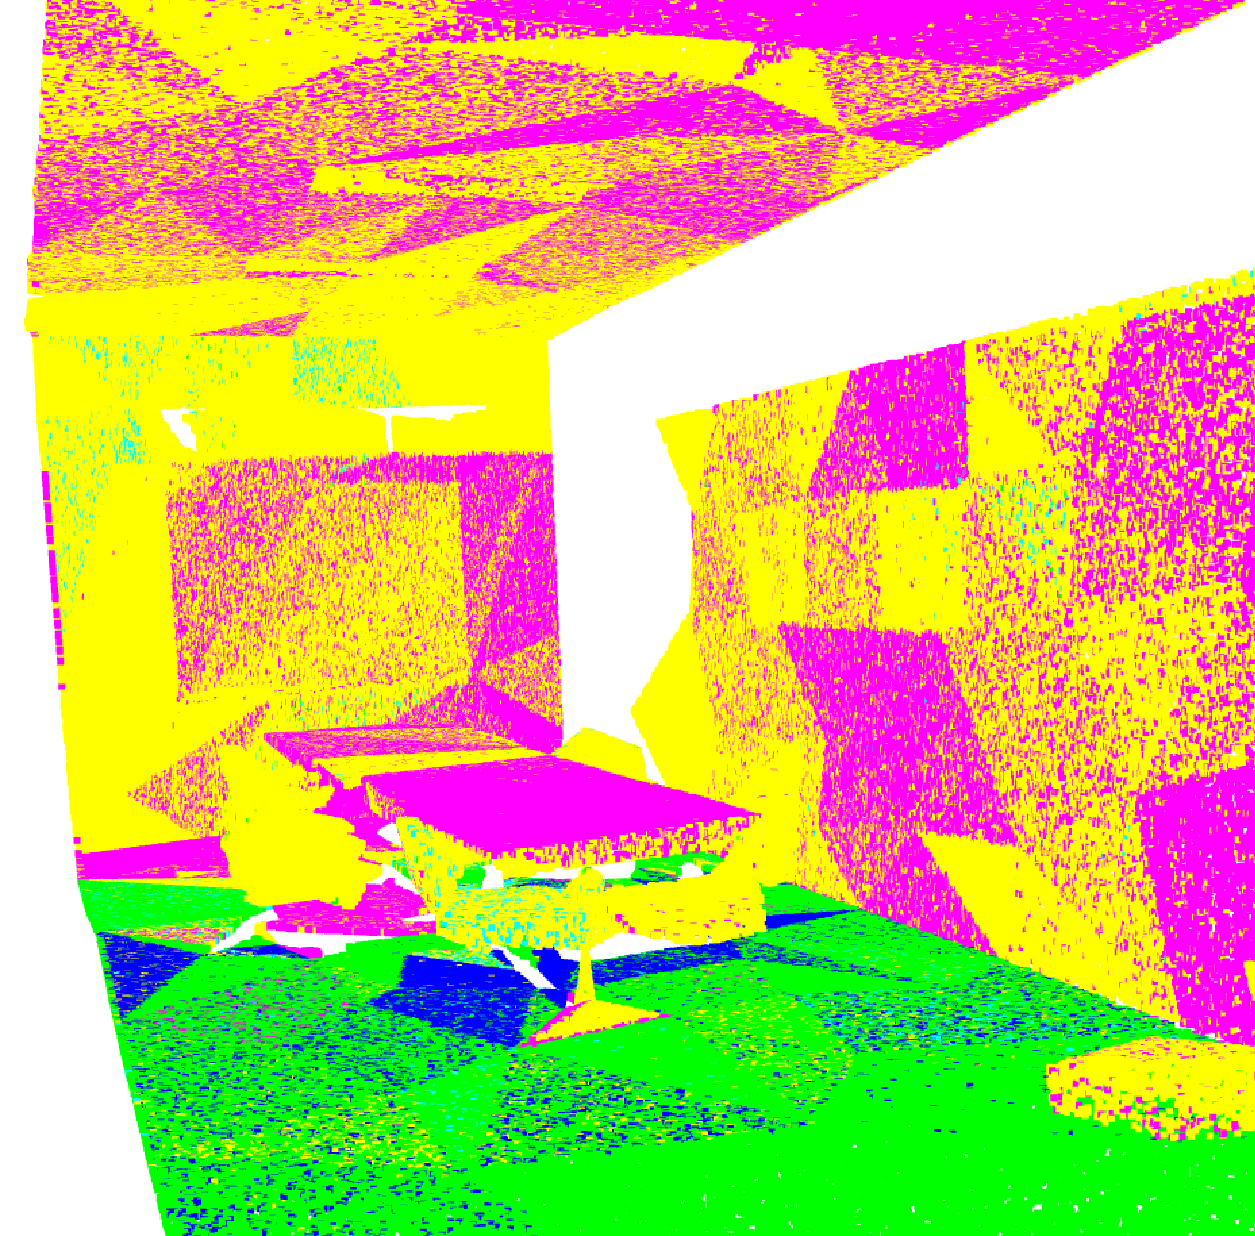
\includegraphics[width=0.33\textwidth, height=0.18\textheight]{images/seg_output/s3dis_DE/ocroom_1.pdf} \\
            
            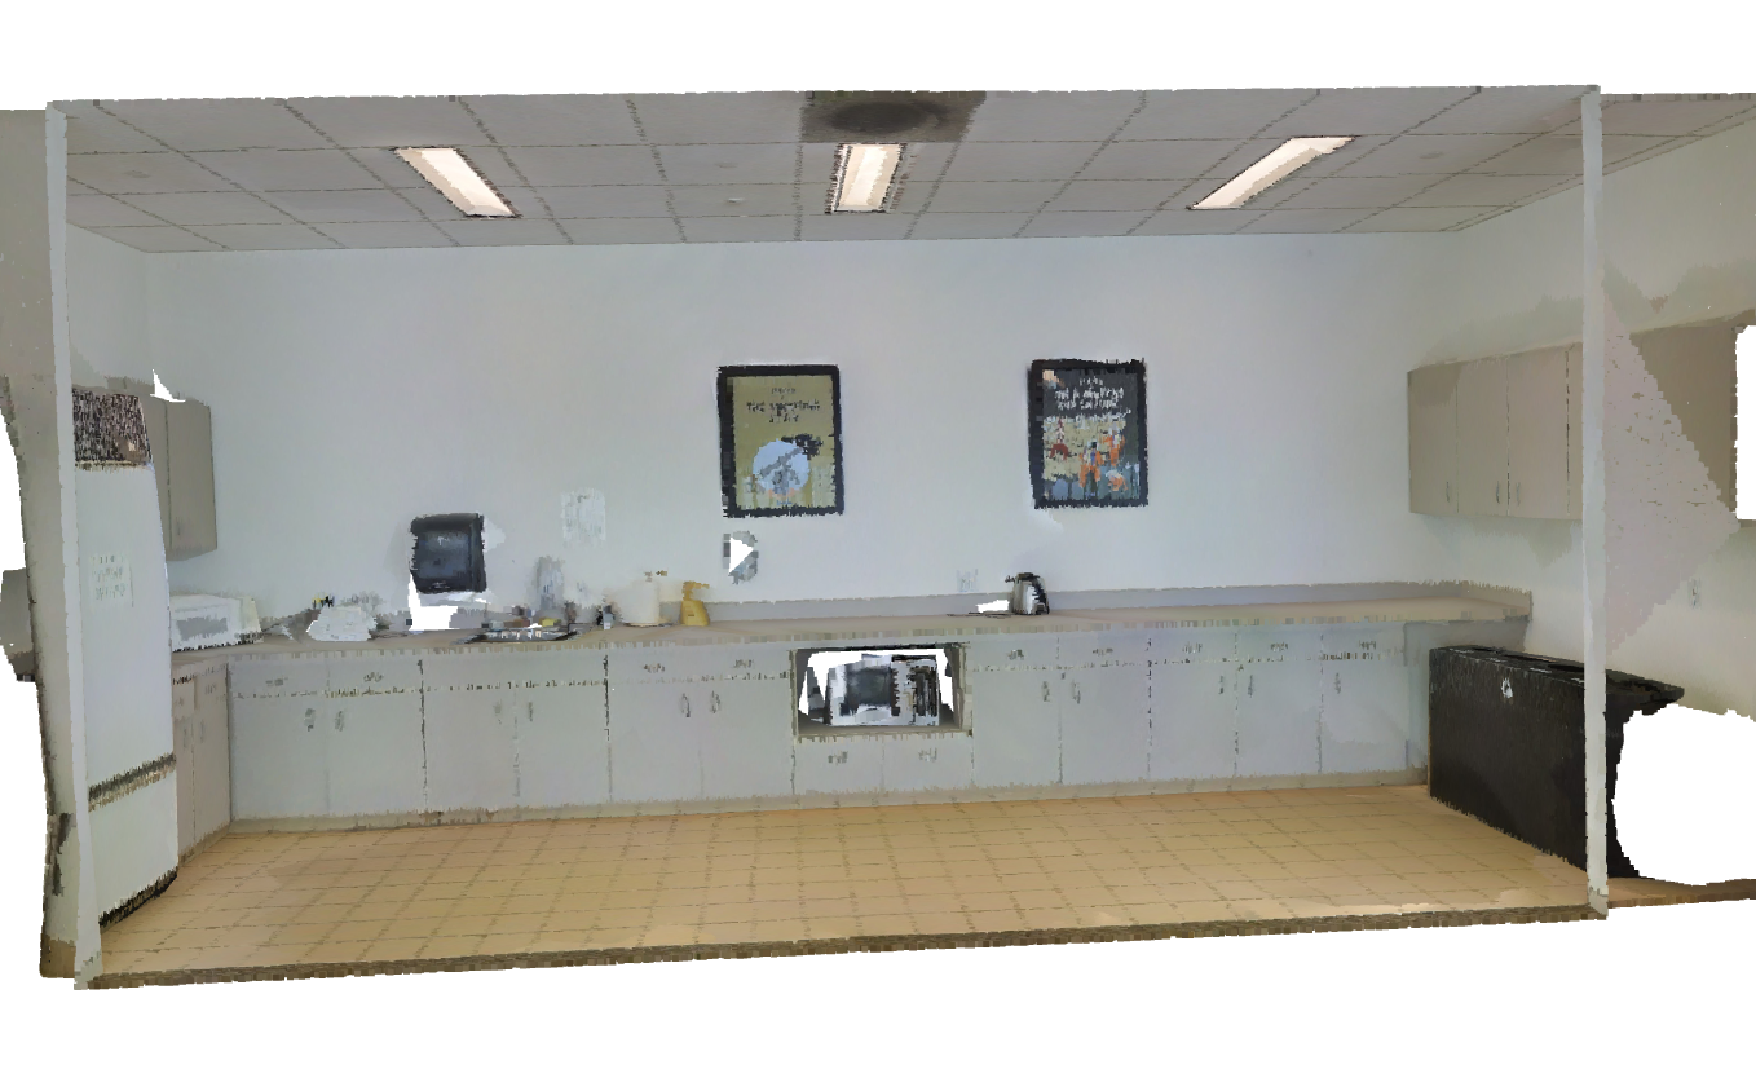
\includegraphics[width=0.33\textwidth, height=0.18\textheight]{images/seg_output/s3dis_DE/S3DIS_3_RGB.pdf} &
            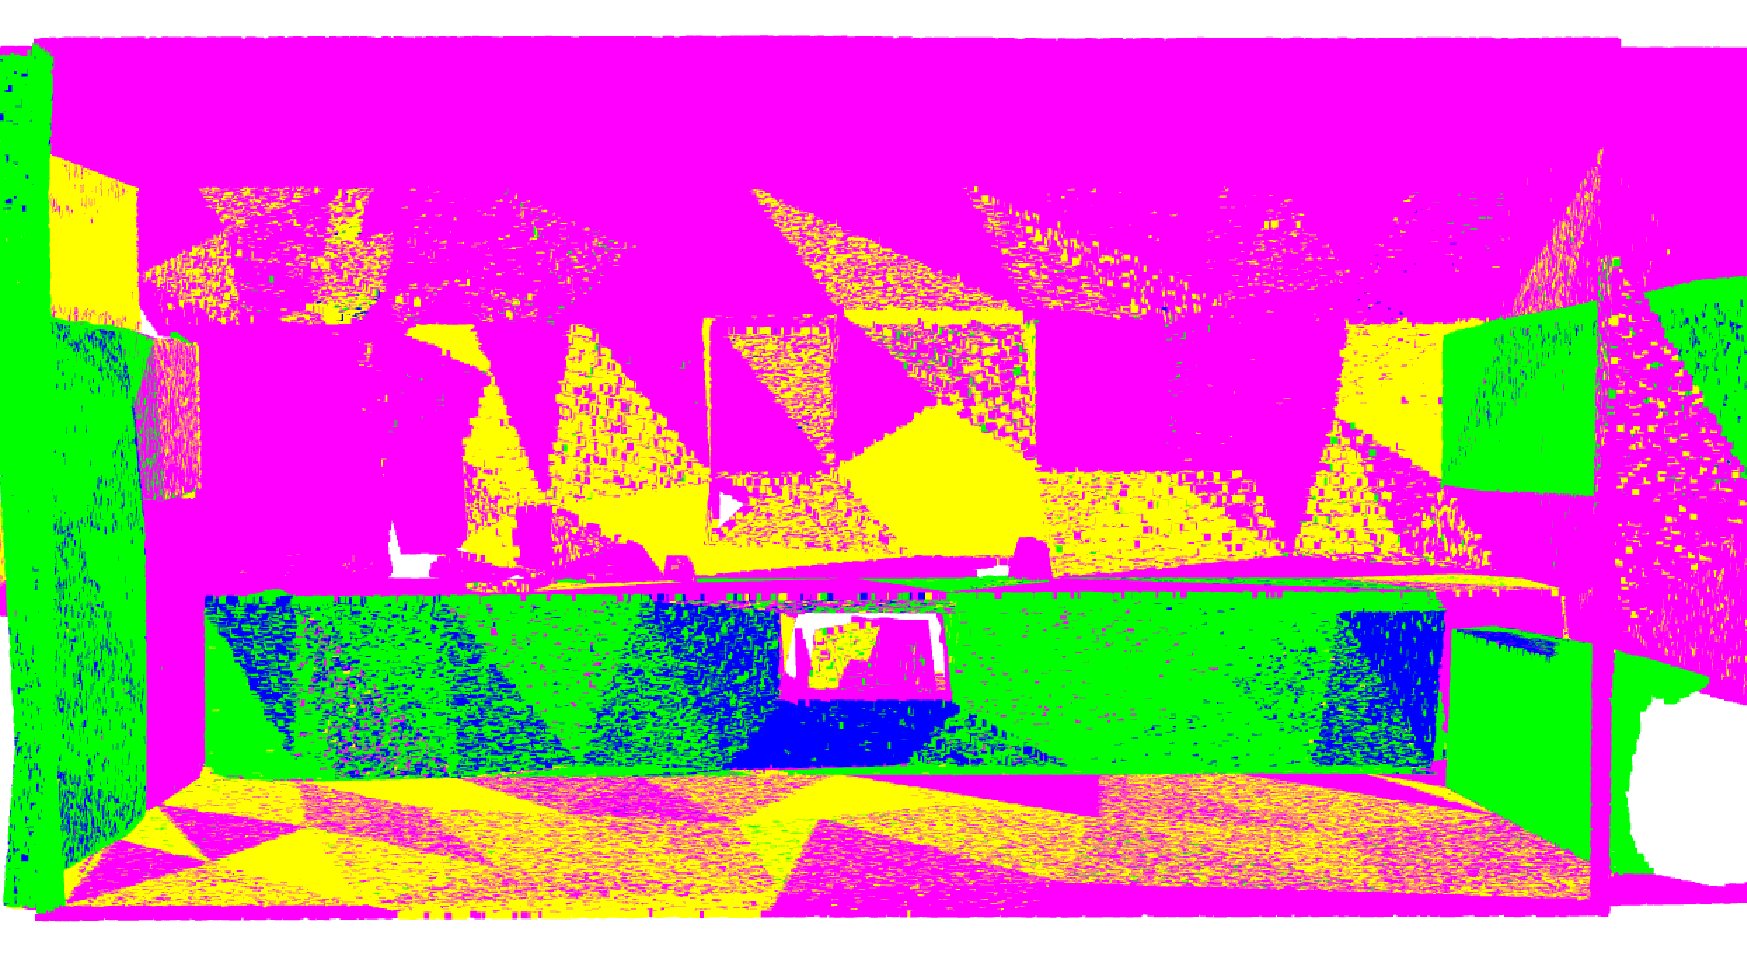
\includegraphics[width=0.33\textwidth, height=0.18\textheight]{images/seg_output/s3dis_DE/S3DIS_3_Pred.pdf}&
            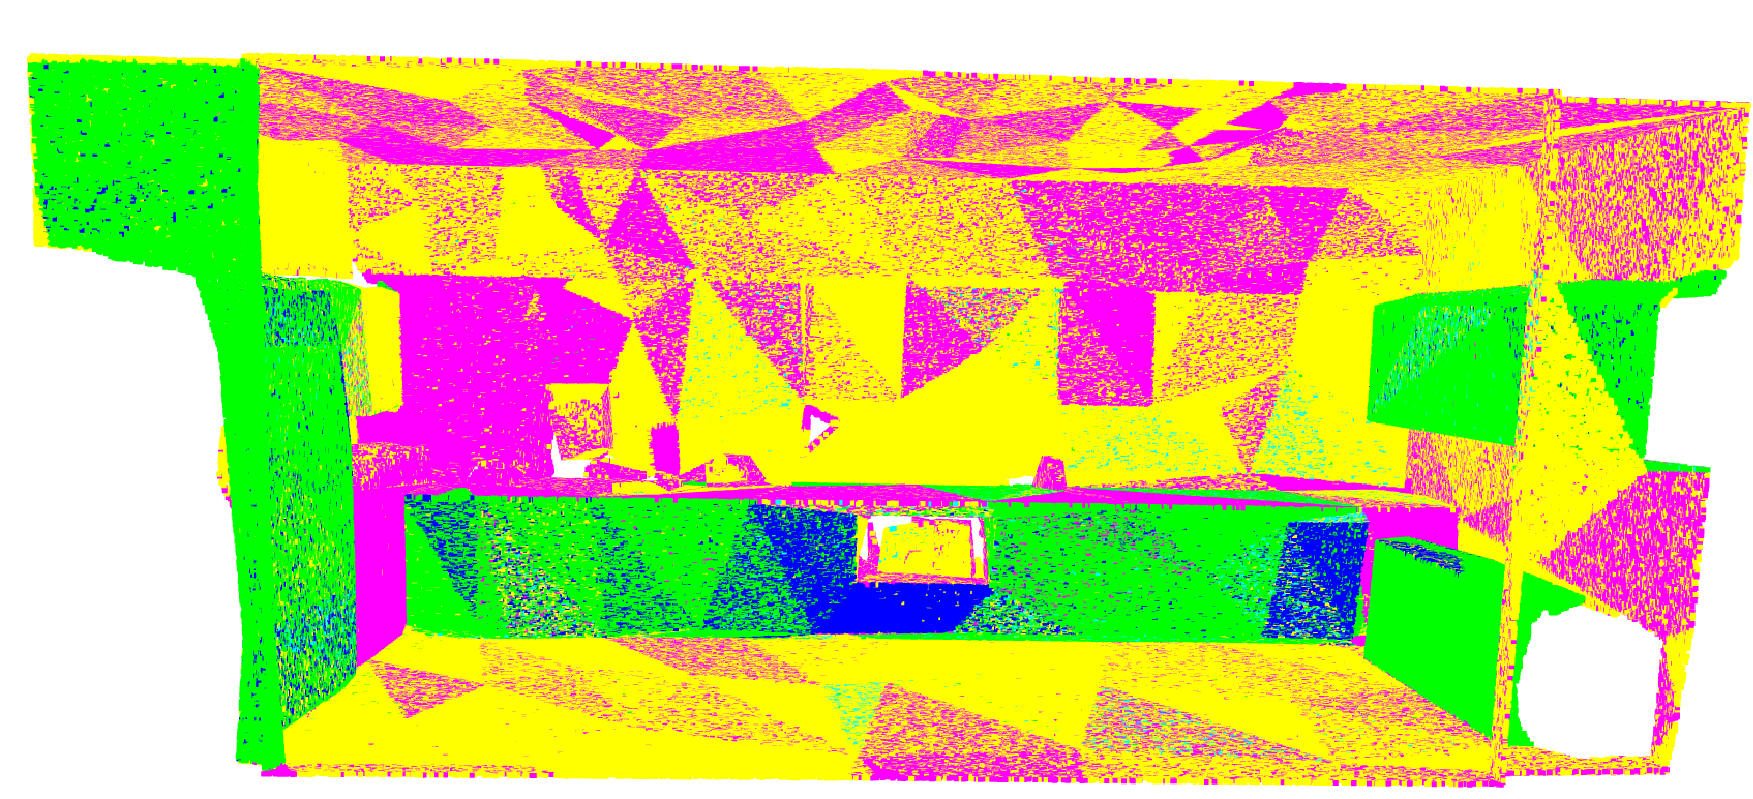
\includegraphics[width=0.33\textwidth, height=0.18\textheight]{images/seg_output/s3dis_DE/opantry_1.pdf} \\

            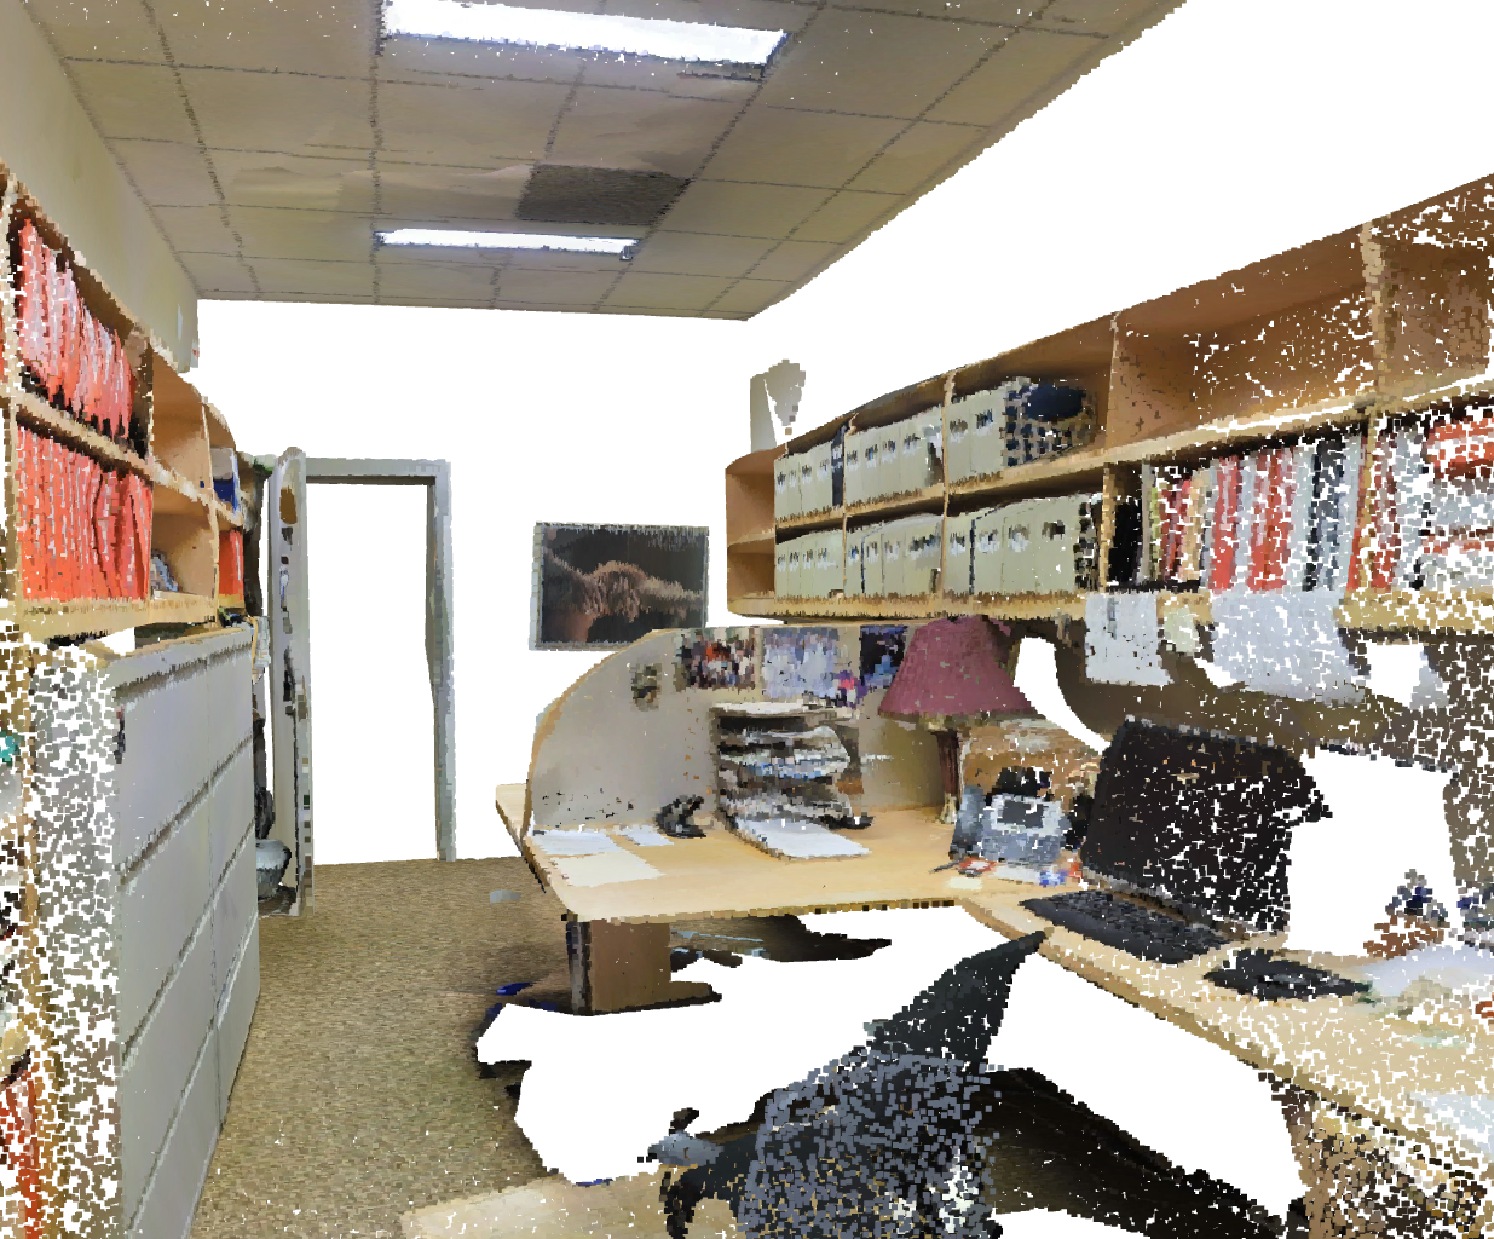
\includegraphics[width=0.33\textwidth, height=0.18\textheight]{images/seg_output/s3dis_DE/S3DIS_4_RGB.pdf} &
            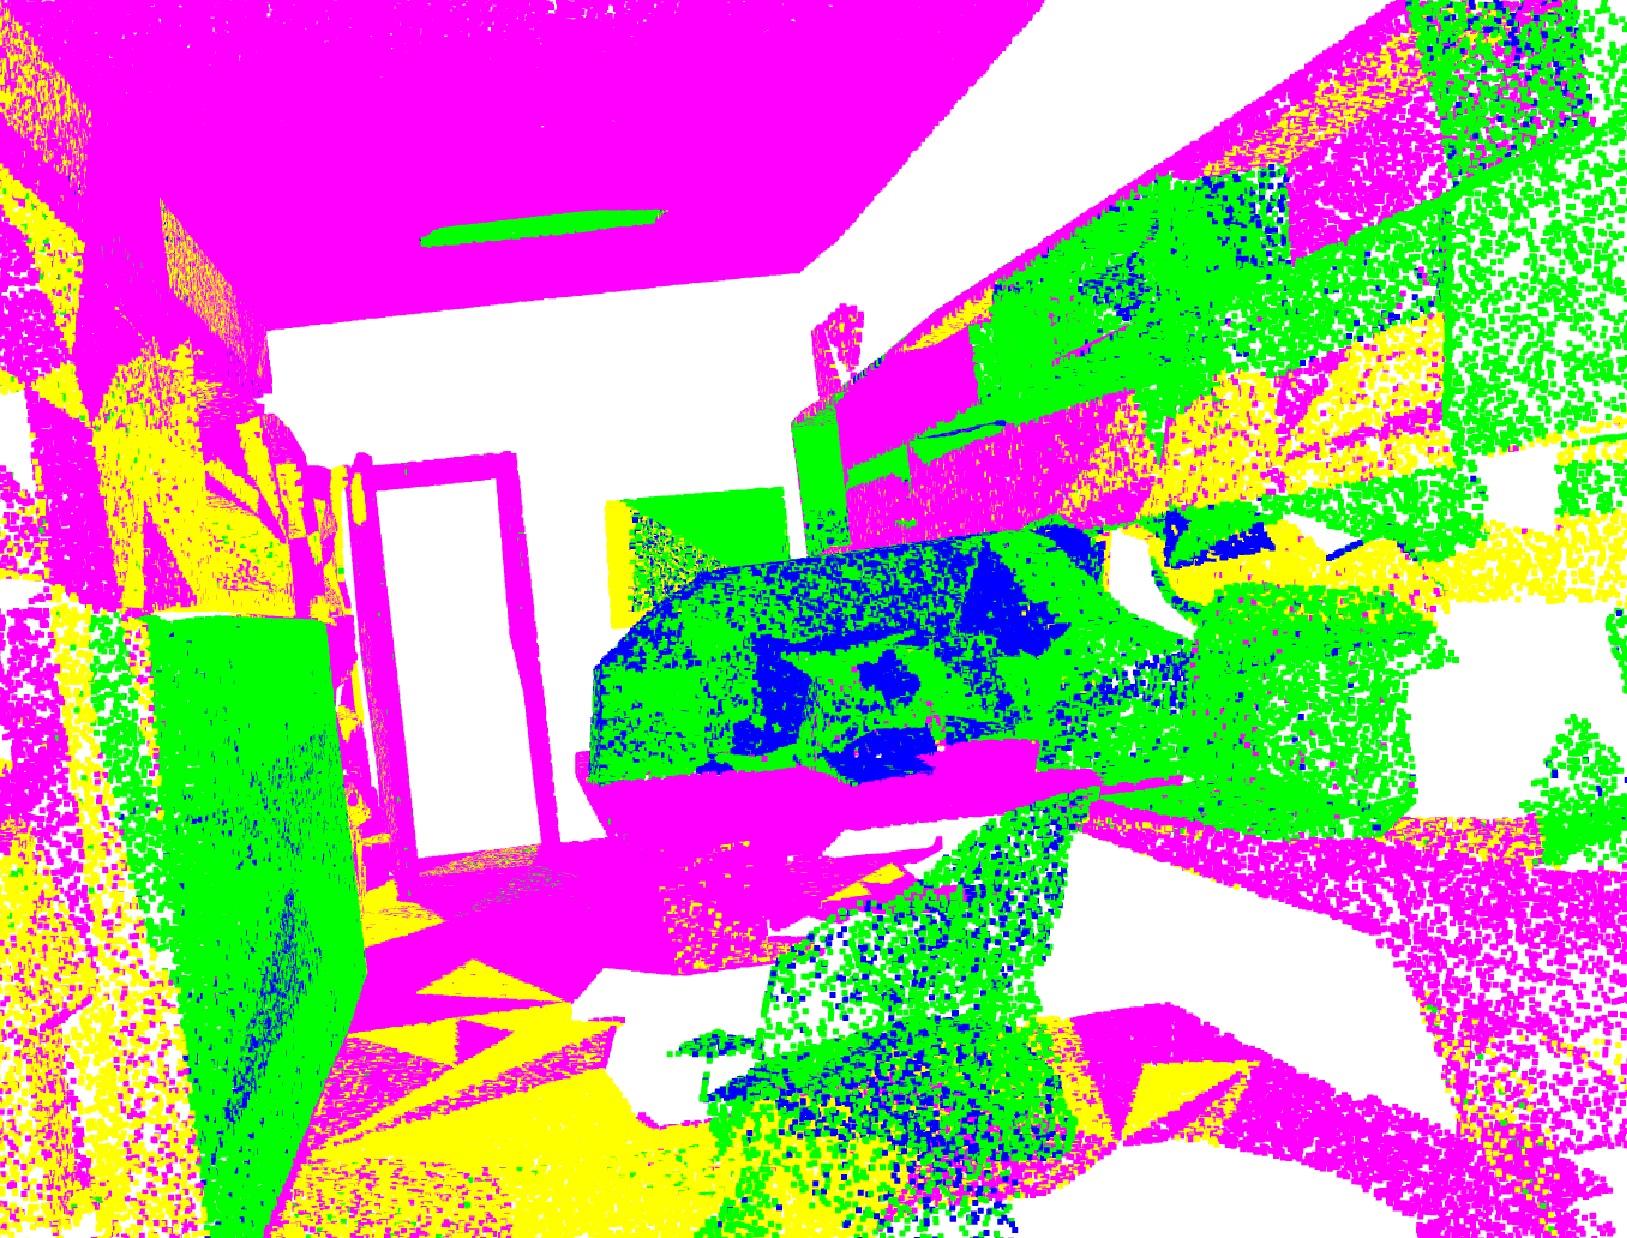
\includegraphics[width=0.33\textwidth, height=0.18\textheight]{images/seg_output/s3dis_DE/S3DIS_4_Pred.pdf}&
            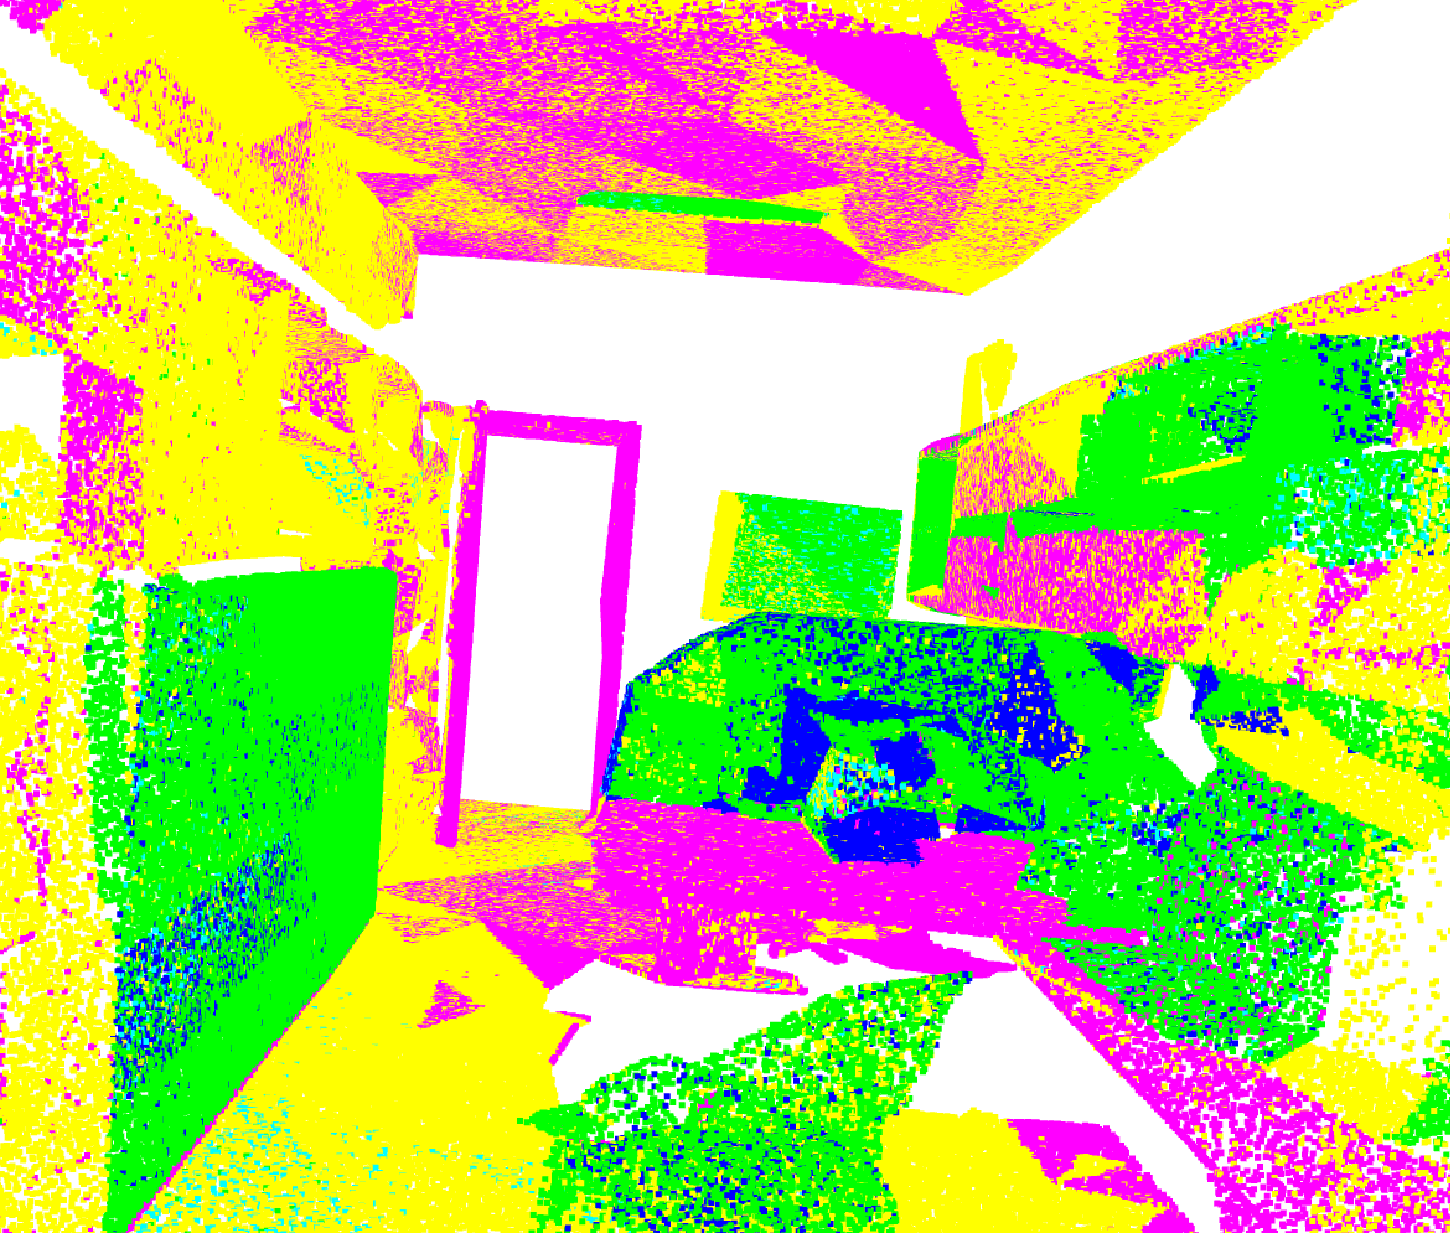
\includegraphics[width=0.33\textwidth, height=0.18\textheight]{images/seg_output/s3dis_DE/office_42.pdf} \\
        \end{tabular}
        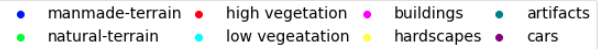
\includegraphics[scale=0.45]{images/legend.png}
        \caption{Predictions of RandLA-Net on S3DIS (OOD) dataset. First column representing the point cloud, second column presenting the predictions of Deep Ensembles and final column represents the results from Flipout model.
        We represented the results with ensemble size of 15 and 15 forward passes for Flipout.}
        \label{fig:de_s3dis_vis}
    \end{figure*}
    \FloatBarrier
    %%%%%% Maximum probability (Semantic3D vs S3DIS) %%%%%%
    \subsection{Maximum Softmax Probability (MSP)}
    \label{sec:prob_sem3dvs3dis}
    In this experiment, we study the probability values of the ID dataset (Semantic3D), and OOD dataset (S3DIS) computed using Deep Ensembles and Flipout methods of RandLA-Net.
    We compute the average of the maximum softmax probability of all the points in the dataset, and this averaged value is called here the mean probability value.
    Figure~\ref{fig:msp_ensembles} and Figure~\ref{fig:msp_flipout} depict the mean probability values across the ID (green) and OOD (red) datasets, and their variance is represented as error bars.
    Figure~\ref{fig:msp_ensembles} represents the change in mean probability value to ensemble size.
    Figure~\ref{fig:msp_flipout} represents the change in mean probability value to the number of passes in Flipout.
    Here, we represent the mean probability score and variance for every fifth ensemble for Deep Ensmebles and fifth forward pass for Flipout.
    \begin{figure}[!ht]
        \begin{subfigure}{0.98\textwidth}
            \centering
        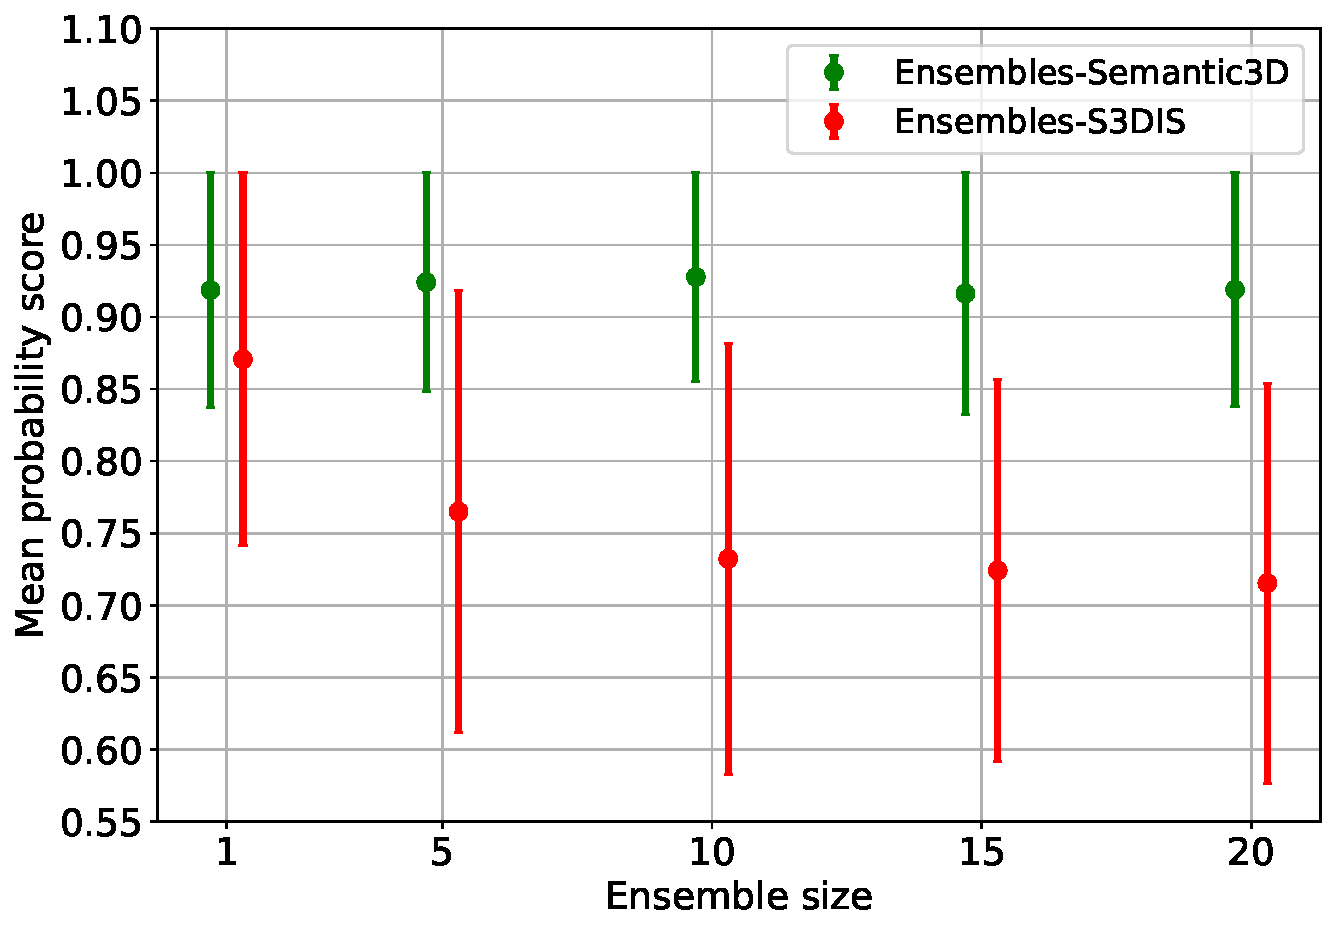
\includegraphics[scale=0.5]{images/MSP/Ensembles_MSP_semvs3d.pdf}
        \caption{}
        \label{fig:msp_ensembles}
        \end{subfigure}
        \begin{subfigure}{0.98\textwidth}
            \centering
        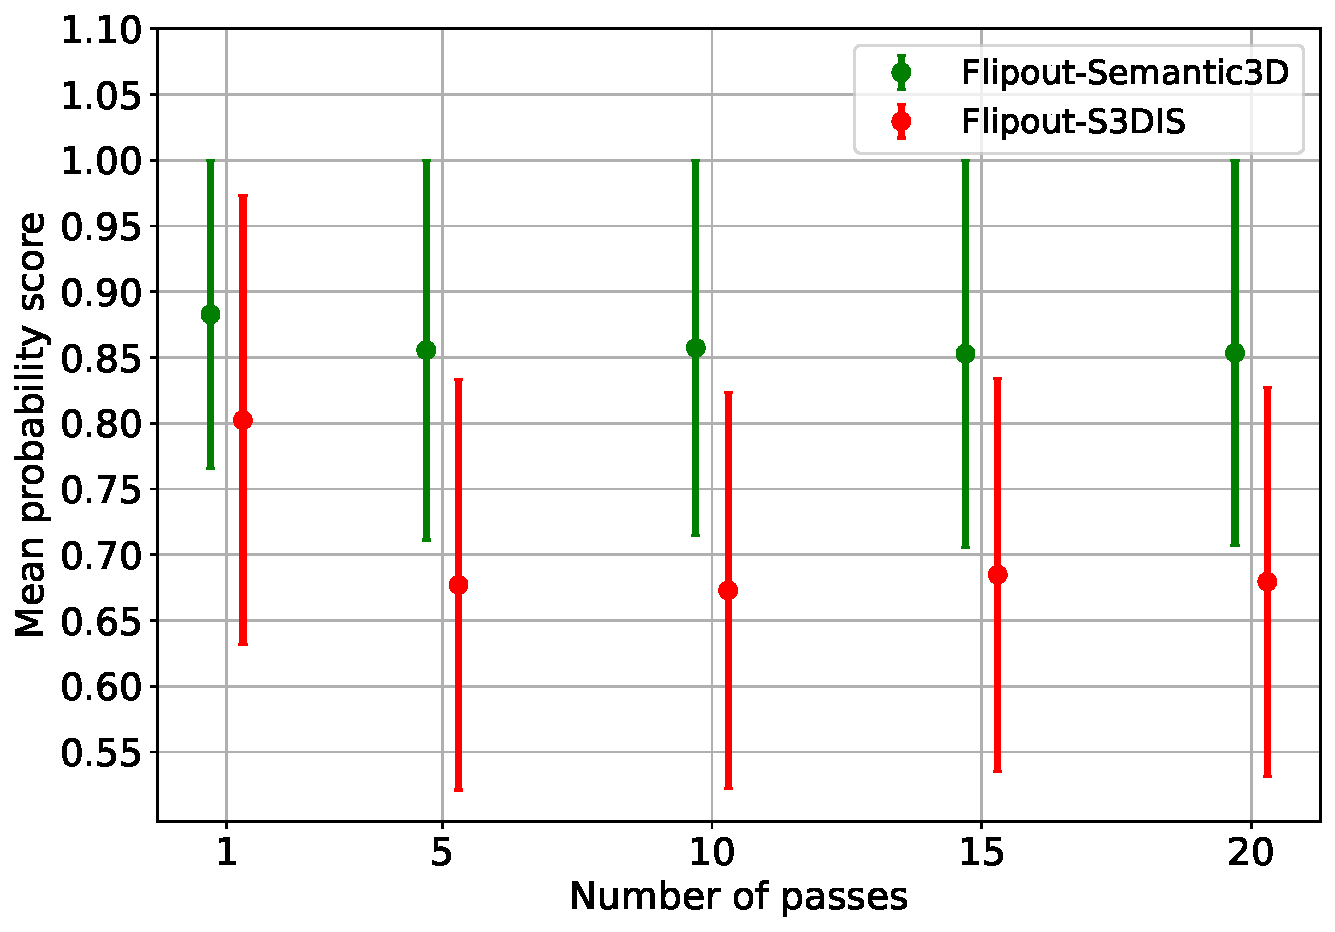
\includegraphics[scale=0.5]{images/MSP/Flipout_MSP_semvs3d.pdf}
        \caption{}
        \label{fig:msp_flipout}
        \end{subfigure}
        \caption{Graph representing the mean probability value as a dot for Semantic3D (ID) in green and S3DIS (OOD) in red. The variance is represented via the error bars.  (a) represents the mean probability value for various ensemble sizes and (b) represents the mean probability value for multiple forward passes on Flipout model.}
    \end{figure}

    From Figure~\ref{fig:msp_ensembles}, we can infer that as the increase in ensemble size, the mean probability of the ID (Semantic3D) dataset remains stable.
    The variance is reduced until the ensemble size of 10 and then stabilizes.
    In the case of the OOD (S3DIS) dataset, we observe a decrement in mean probability value and then remain the same after an ensemble size of 5 with a larger variance.
    With the increase in ensemble size, we also observe that the overlap in the variance of ID and OOD is getting lower.
    This smaller overlap in higher ensemble sizes should result in higher OOD detection performance.
    In the case of Flipout, as in Figure~\ref{fig:msp_flipout} the mean probability and variance remain mostly the same for the ID dataset.
    With the OOD dataset, we observed a reduction in the mean probability value in the case of multiple passes.
    The variance from the Flipout is higher than the Deep Ensembles for the ID dataset.
    This phenomenon is to be expected because the Deep Ensembles combine predictions from various randomly initialized models.
    In the case of Flipout, the same model is used for multiple forward passes.

    Figure~\ref{fig:de_sem3d_probmap} and Figure~\ref{fig:fout_sem3d_probmap} represent the ground truth, prediction and probability map of the ID (Semantic3D) dataset using Deep Ensembles and Flipout respectively.
    Similarly, Figure~\ref{fig:de_s3dis_probmap} and Figure~\ref{fig:fout_s3dis_probmap} depict the prediction and probability map for the OOD (S3DIS) dataset using Deep Ensembles and Flipout respectively.
    On visual inspection of Figure~\ref{fig:de_sem3d_probmap} and Figure~\ref{fig:fout_sem3d_probmap}, we observed that the probability scores are low for points that are misclassified for ID dataset.
    The points which lie on the edge of the structures are low scored.
    This effect is profound near the edges of the church and the edges of the walls.
    In the case of the OOD dataset presented in Figure~\ref{fig:de_s3dis_probmap} and Figure~\ref{fig:fout_s3dis_probmap}, the overall probability scores are low, as the whole point cloud has a greener shade than the ID dataset probability map represented in a yellow shade.

    \begin{figure*}[h!]
        \centering
        \begin{tabular}{ccc}
            Ground Truth & Prediction-Deep Ensembles & Probability map-Deep Ensembles \\
            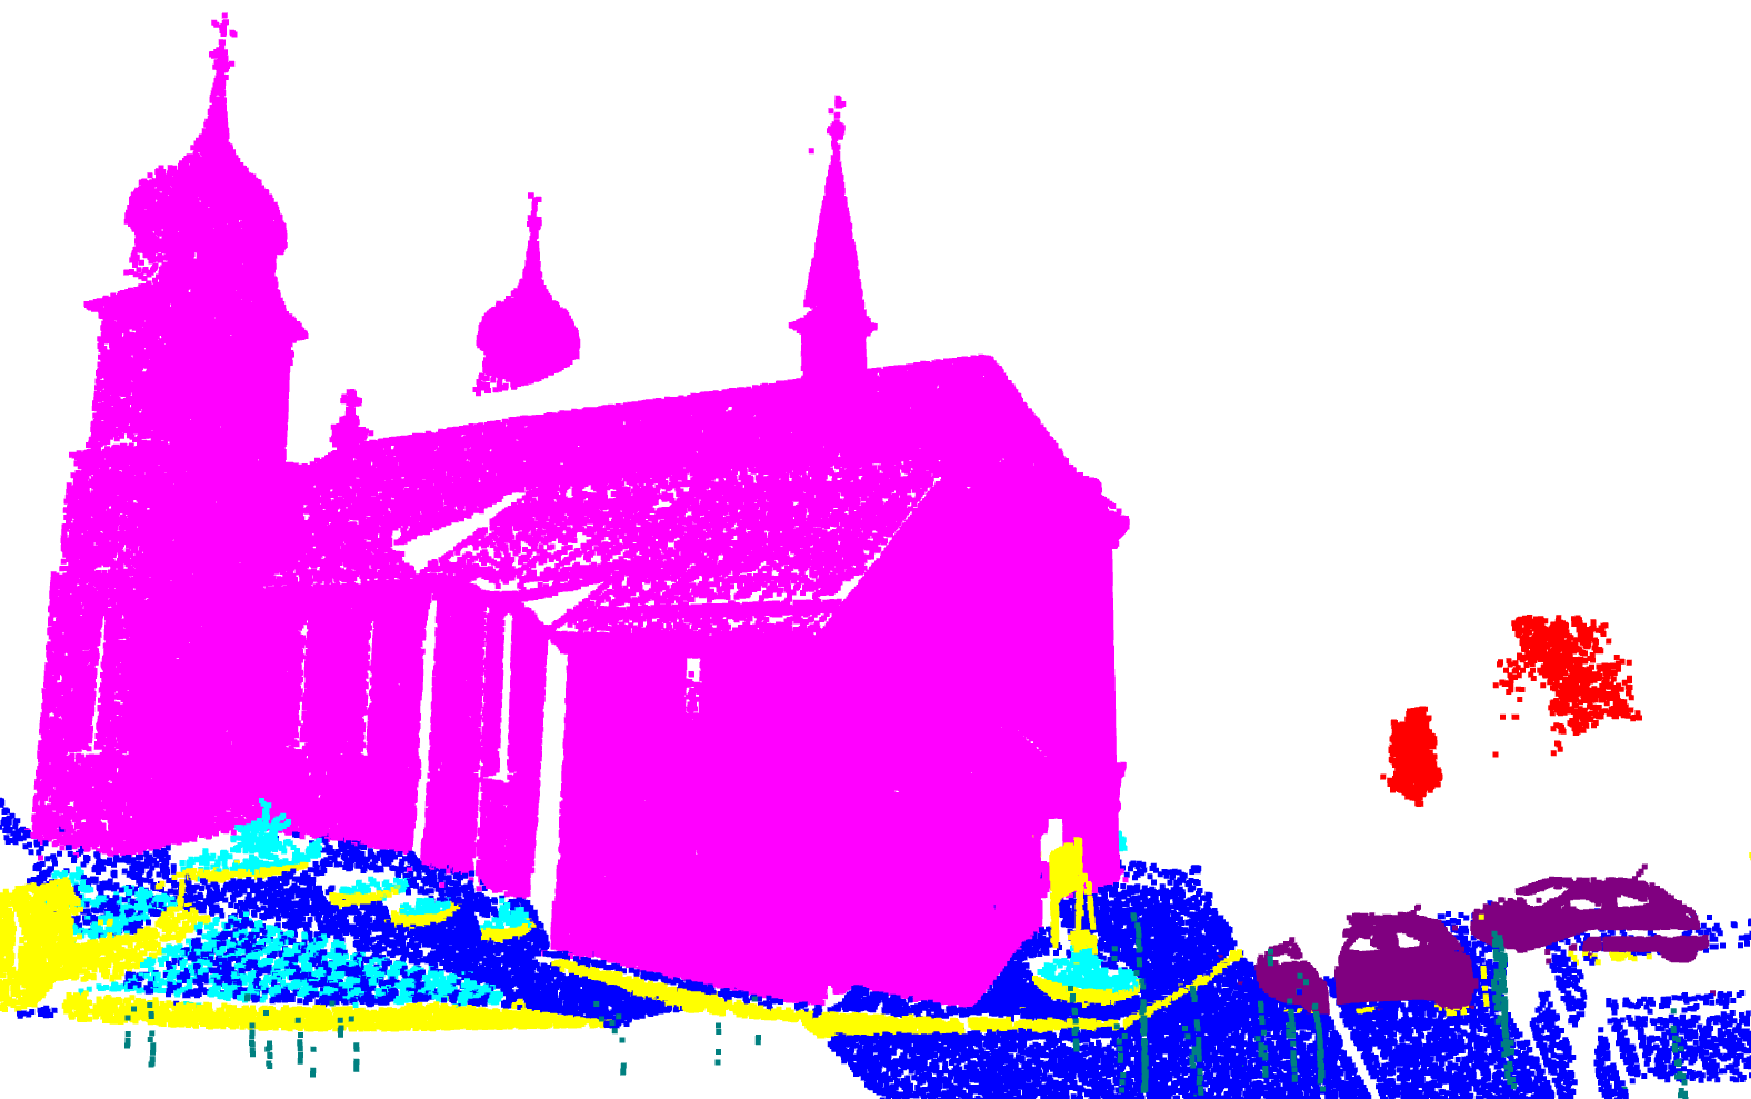
\includegraphics[width=0.33\textwidth, height=0.18\textheight]{images/seg_output/sem3d_seg_output/1_GT.pdf} &
            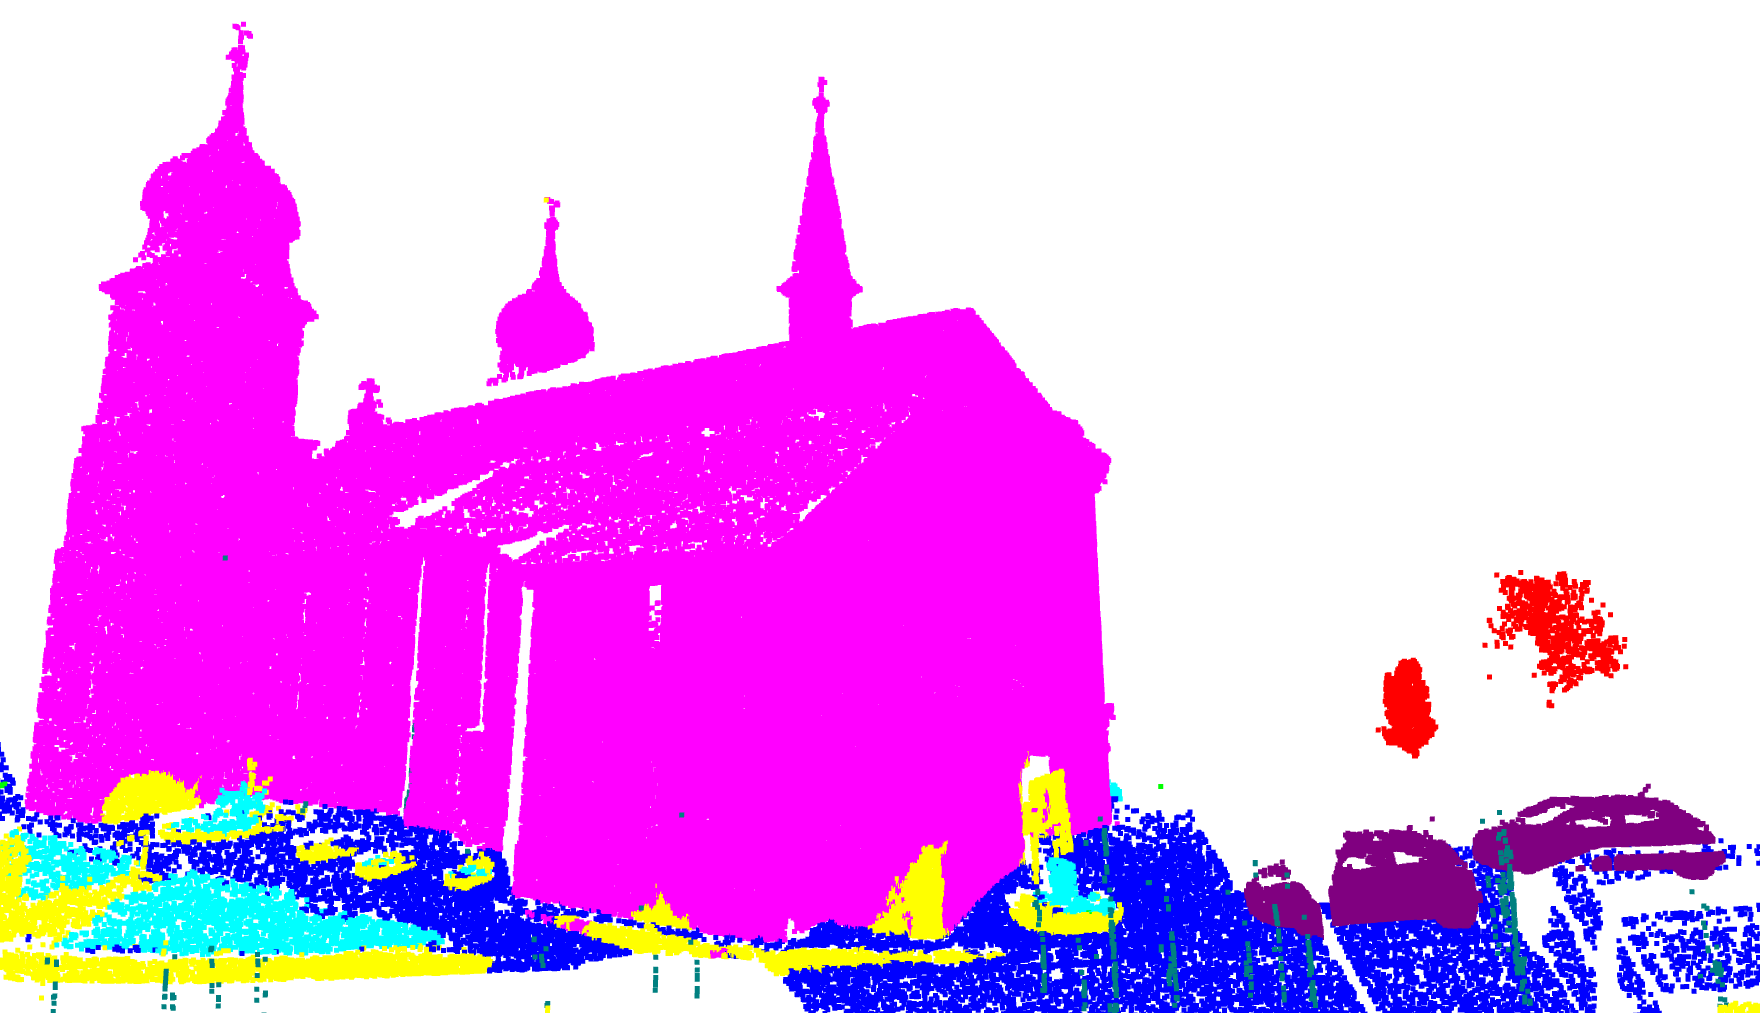
\includegraphics[width=0.33\textwidth, height=0.18\textheight]{images/seg_output/sem3d_seg_output/1_Pred.pdf}& 
            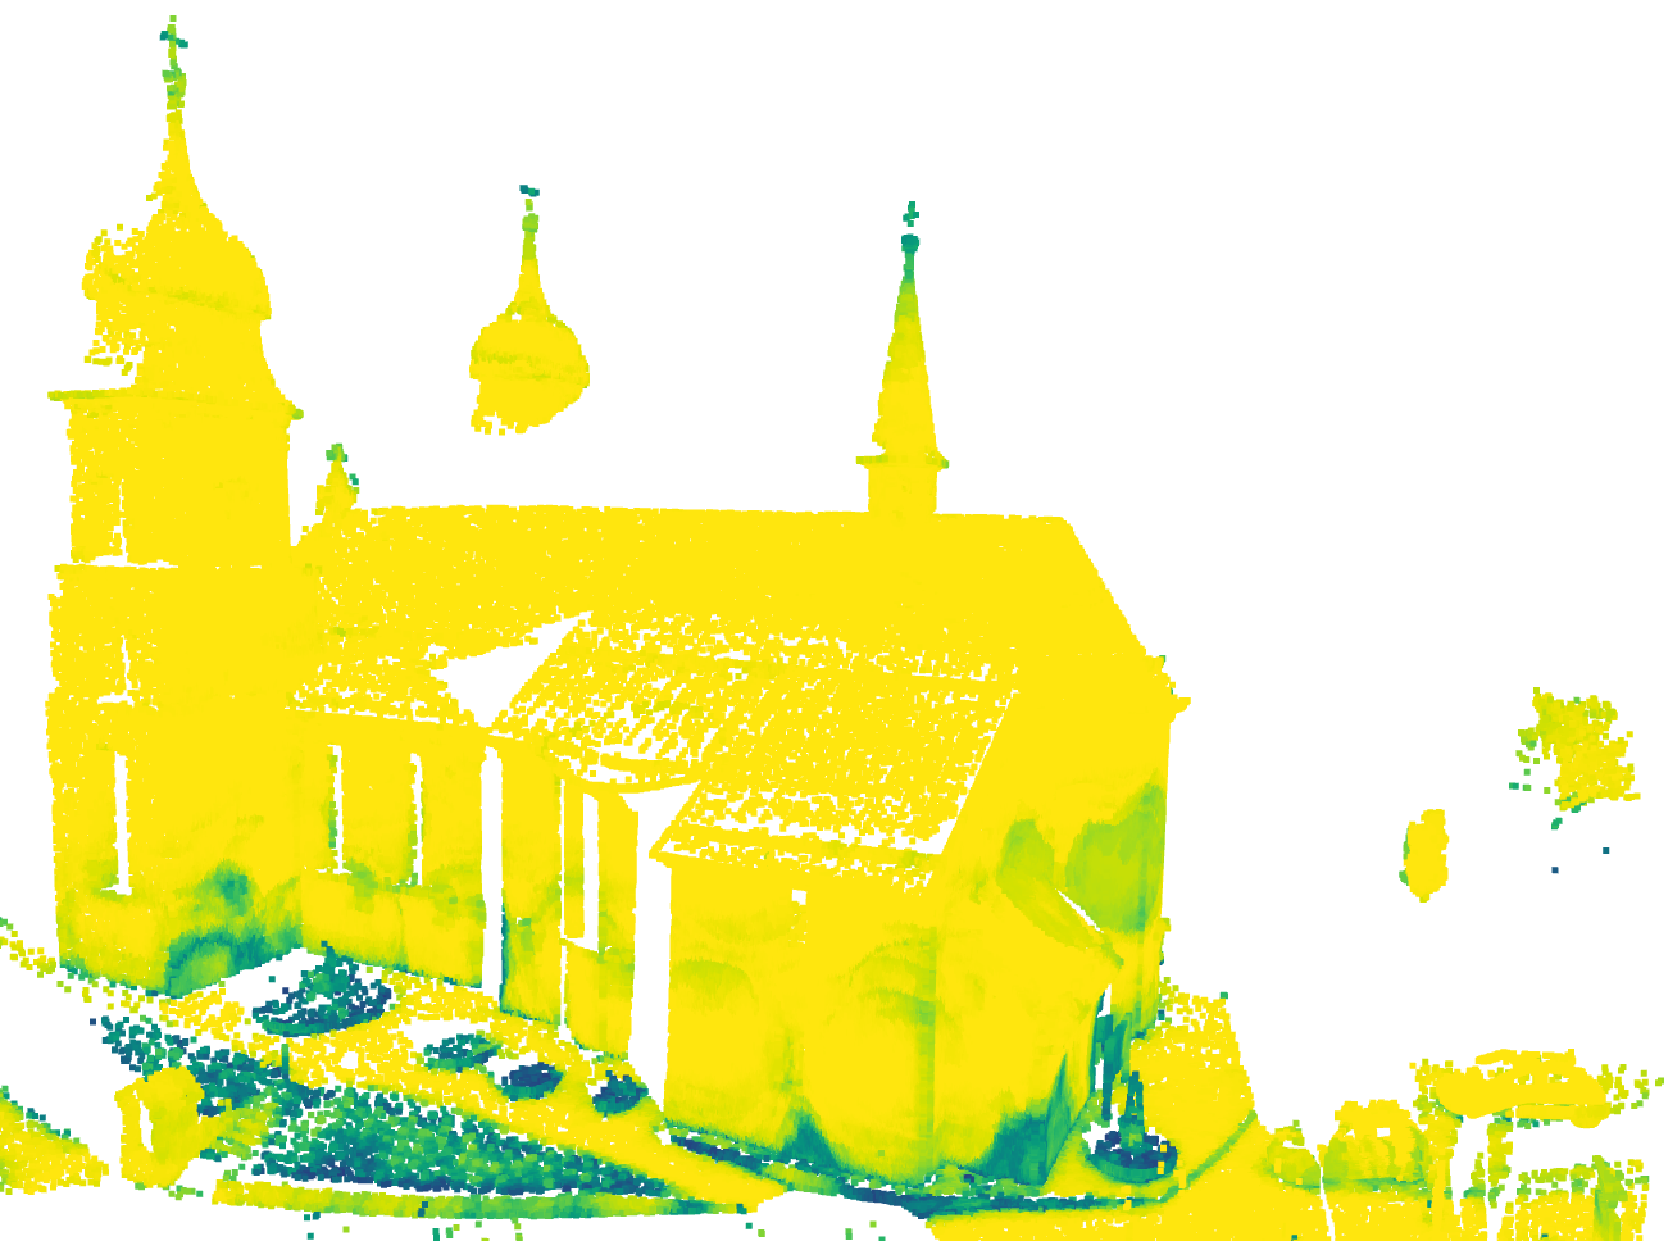
\includegraphics[width=0.33\textwidth, height=0.18\textheight]{images/seg_output/sem3d_seg_output/1_max_prob.pdf}\\

            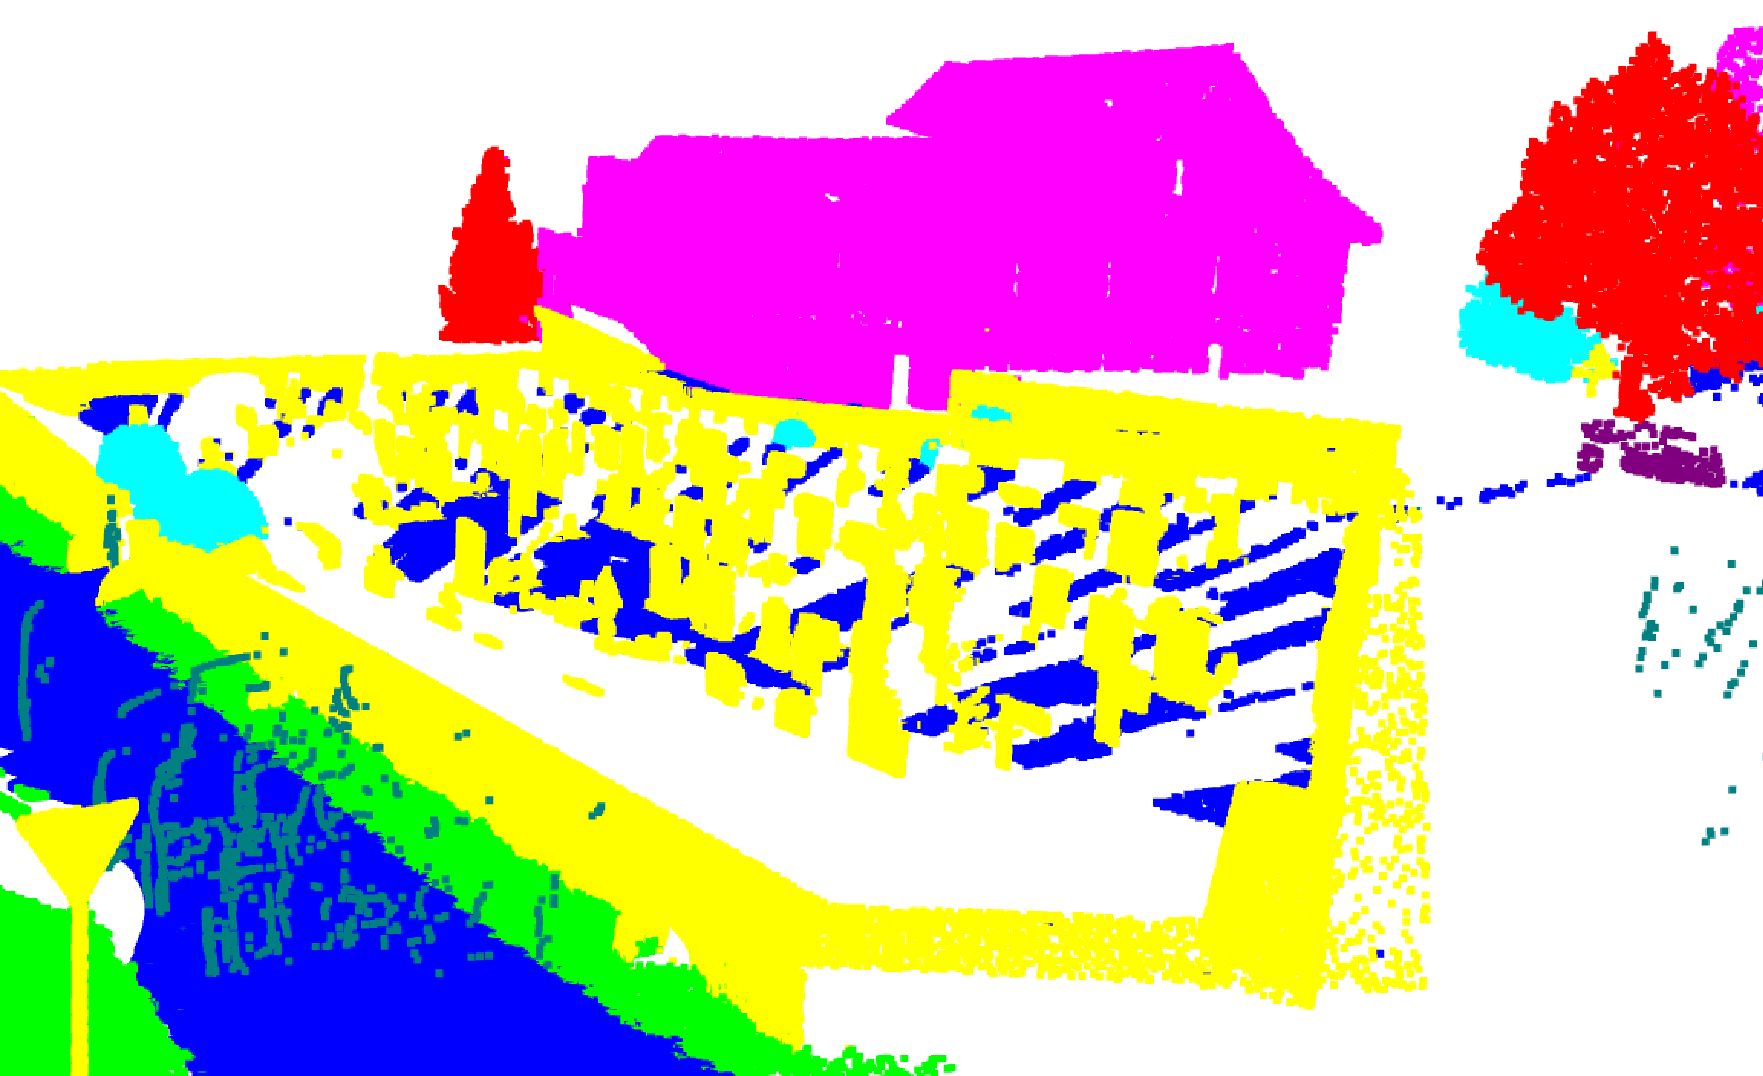
\includegraphics[width=0.33\textwidth, height=0.18\textheight]{images/seg_output/sem3d_seg_output/2_GT.pdf} &
            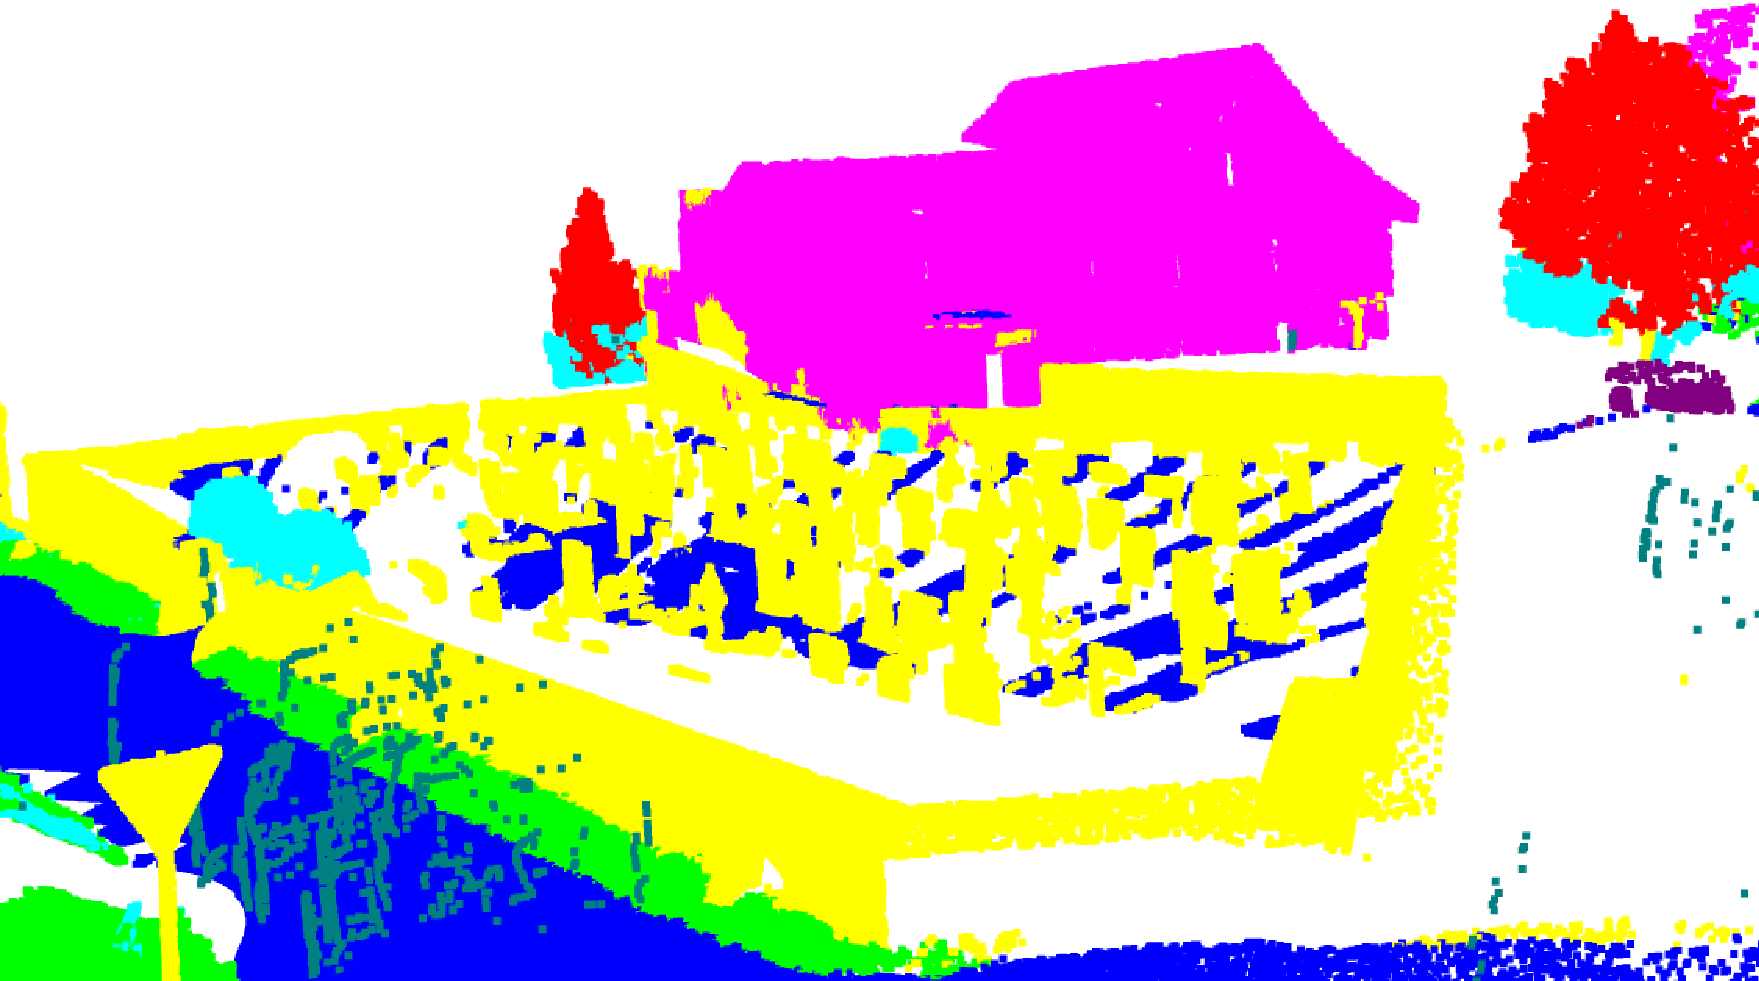
\includegraphics[width=0.33\textwidth, height=0.18\textheight]{images/seg_output/sem3d_seg_output/2_Pred.pdf}& 
            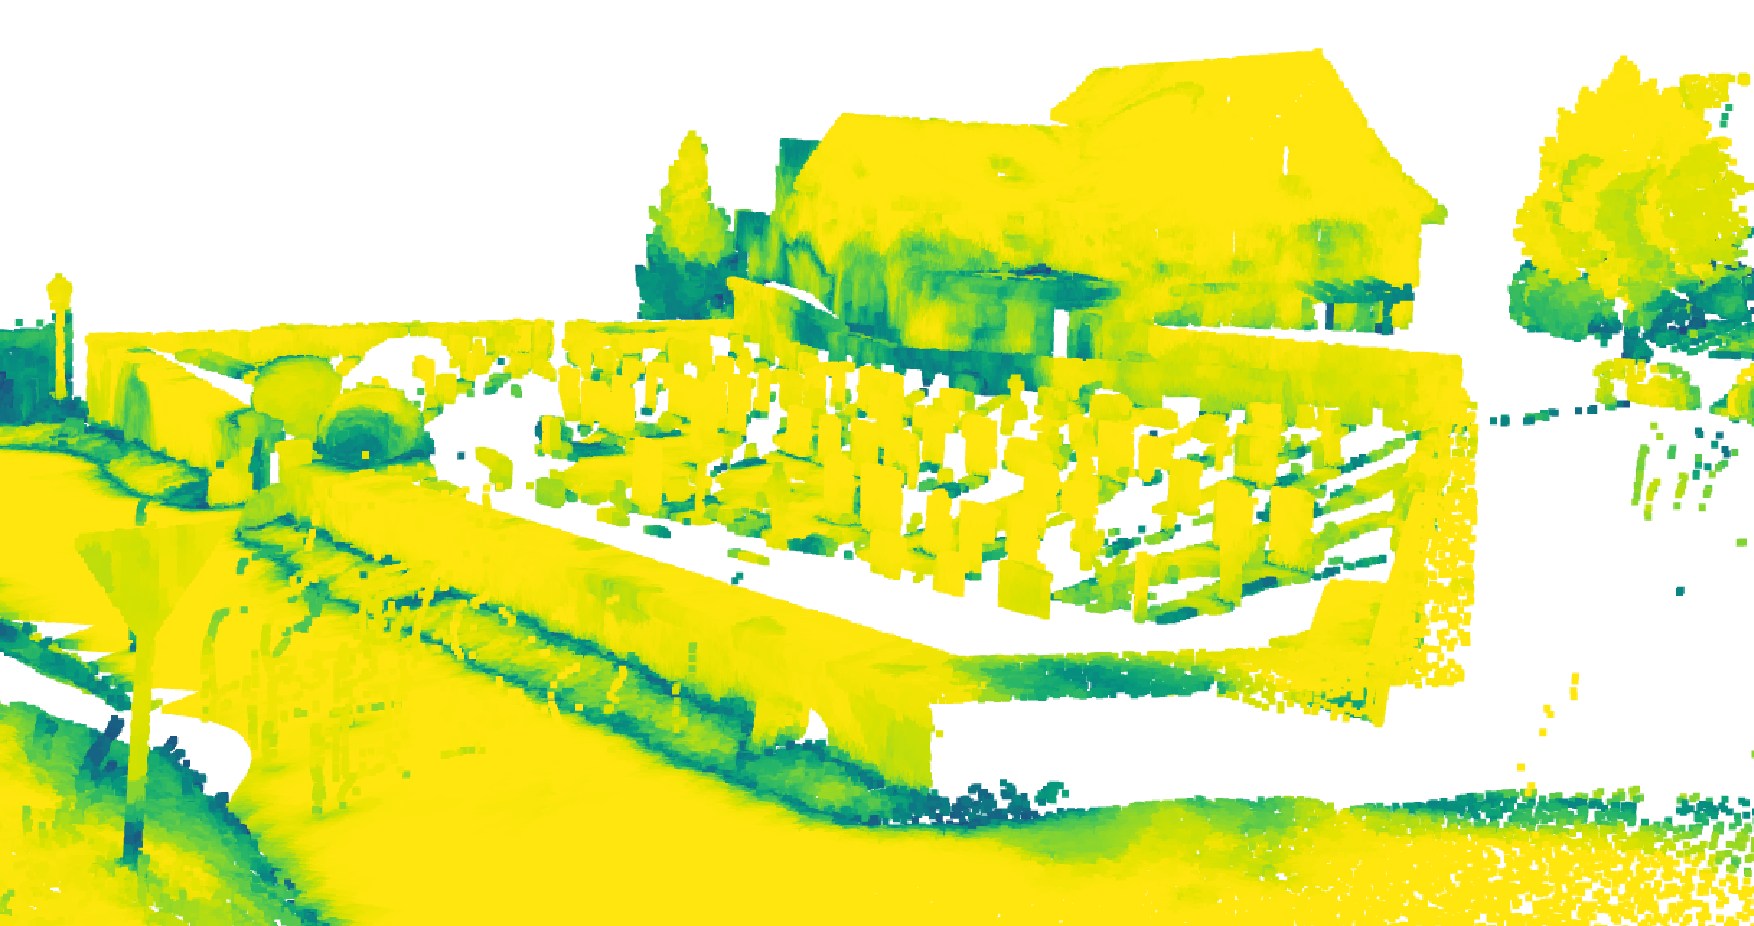
\includegraphics[width=0.33\textwidth, height=0.18\textheight]{images/seg_output/sem3d_seg_output/2_max_prob.pdf}\\

            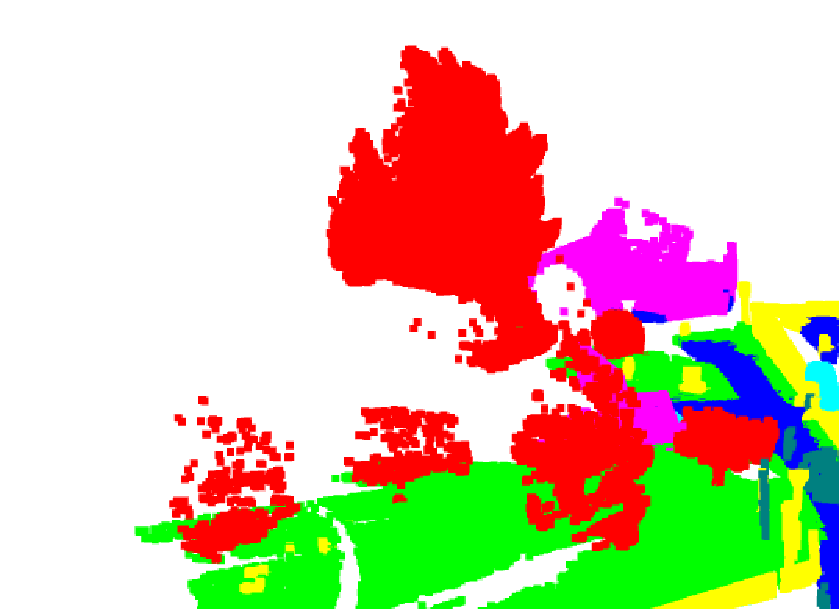
\includegraphics[width=0.33\textwidth, height=0.18\textheight]{images/seg_output/sem3d_seg_output/3_GT.pdf} &
            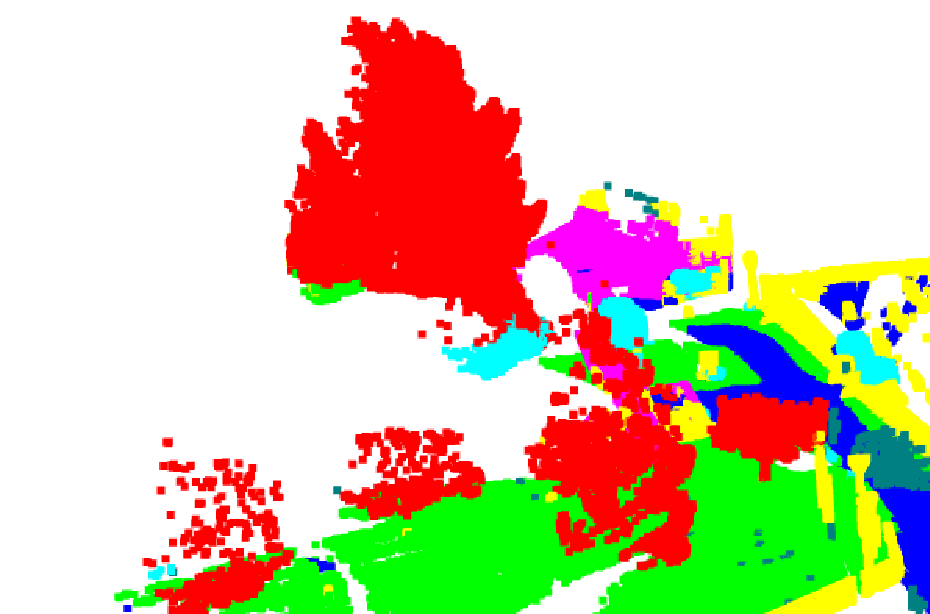
\includegraphics[width=0.33\textwidth, height=0.18\textheight]{images/seg_output/sem3d_seg_output/3_Pred.pdf}& 
            \includegraphics[width=0.33\textwidth, height=0.18\textheight]{images/seg_output/sem3d_seg_output/3_max_prob.pdf}\\
        \end{tabular}
        \includegraphics[scale=0.45]{images/prob_legend.pdf}
        \includegraphics[scale=0.45]{images/legend.png}
        \caption{Image depicts the ground truth, corresponding prediction and per point probability estimated using Deep Ensembles (ensemble size of 15) of various scenes in Semantic3D dataset.}
        \label{fig:de_sem3d_probmap}
    \end{figure*}

    \begin{figure*}[h!]
        \centering
        \begin{tabular}{ccc}
            Ground Truth & Prediction-Flipout & Probability map-Flipout \\
            \includegraphics[width=0.33\textwidth, height=0.18\textheight]{images/seg_output/sem3d_seg_output/1_GT.pdf} &
            \includegraphics[width=0.33\textwidth, height=0.18\textheight]{images/seg_output/flipout/sem3d_1.pdf}& 
            \includegraphics[width=0.33\textwidth, height=0.18\textheight]{images/seg_output/flipout/1_fout_prob.pdf}\\

            \includegraphics[width=0.33\textwidth, height=0.18\textheight]{images/seg_output/sem3d_seg_output/2_GT.pdf} &
            \includegraphics[width=0.33\textwidth, height=0.18\textheight]{images/seg_output/flipout/sem3d_2.pdf}& 
            \includegraphics[width=0.33\textwidth, height=0.18\textheight]{images/seg_output/flipout/2_fout_prob.pdf}\\

            \includegraphics[width=0.33\textwidth, height=0.18\textheight]{images/seg_output/sem3d_seg_output/3_GT.pdf} &
            \includegraphics[width=0.33\textwidth, height=0.18\textheight]{images/seg_output/flipout/sem3d_3.pdf}& 
            \includegraphics[width=0.33\textwidth, height=0.18\textheight]{images/seg_output/flipout/3_fout_prob.pdf}\\
        \end{tabular}
        \includegraphics[scale=0.45]{images/prob_legend.pdf}
        \includegraphics[scale=0.45]{images/legend.png}
        \caption{Image depicts the ground truth, corresponding prediction and per point probability estimated using Flipout (forward passes of 15) of various scenes in Semantic3D dataset.}
        \label{fig:fout_sem3d_probmap}
    \end{figure*}

    \begin{figure*}[h!]
        \centering
        \begin{tabular}{cc}
            Prediction-Deep Ensembles & Probability map-Deep Ensembles \\
            \includegraphics[width=0.33\textwidth, height=0.18\textheight]{images/seg_output/s3dis_DE/S3DIS_1_Pred.pdf}& 
            \includegraphics[width=0.33\textwidth, height=0.18\textheight]{images/seg_output/s3dis_DE/S3DIS_1_prob.pdf}\\

            \includegraphics[width=0.33\textwidth, height=0.18\textheight]{images/seg_output/s3dis_DE/S3DIS_2_Pred.pdf}& 
            \includegraphics[width=0.33\textwidth, height=0.18\textheight]{images/seg_output/s3dis_DE/S3DIS_2_prob.pdf}\\

            \includegraphics[width=0.33\textwidth, height=0.18\textheight]{images/seg_output/s3dis_DE/S3DIS_3_Pred.pdf}& 
            \includegraphics[width=0.33\textwidth, height=0.18\textheight]{images/seg_output/s3dis_DE/S3DIS_3_prob.pdf}\\

            \includegraphics[width=0.33\textwidth, height=0.18\textheight]{images/seg_output/s3dis_DE/S3DIS_4_Pred.pdf}& 
            \includegraphics[width=0.33\textwidth, height=0.18\textheight]{images/seg_output/s3dis_DE/S3DIS_4_prob.pdf}\\
        \end{tabular}
        \includegraphics[scale=0.45]{images/prob_legend.pdf}
        \includegraphics[scale=0.45]{images/legend.png}
        \caption{Image depicts the prediction and per point probability estimated using Deep Ensembles (ensemble size of 15) of various scenes in S3DIS (OOD) dataset.}
        \label{fig:de_s3dis_probmap}
    \end{figure*}

    \begin{figure*}[h!]
        \centering
        \begin{tabular}{cc}
            Prediction-Flipout & Probability map-Flipout \\
            \includegraphics[width=0.33\textwidth, height=0.18\textheight]{images/seg_output/s3dis_DE/office_3.pdf}& 
            \includegraphics[width=0.33\textwidth, height=0.18\textheight]{images/seg_output/s3dis_DE/fout_1.pdf}\\

            \includegraphics[width=0.33\textwidth, height=0.18\textheight]{images/seg_output/s3dis_DE/ocroom_1.pdf}& 
            \includegraphics[width=0.33\textwidth, height=0.18\textheight]{images/seg_output/s3dis_DE/fout_2.pdf}\\

            \includegraphics[width=0.33\textwidth, height=0.18\textheight]{images/seg_output/s3dis_DE/opantry_1.pdf}& 
            \includegraphics[width=0.33\textwidth, height=0.18\textheight]{images/seg_output/s3dis_DE/fout_3.pdf}\\

            \includegraphics[width=0.33\textwidth, height=0.18\textheight]{images/seg_output/s3dis_DE/office_42.pdf}& 
            \includegraphics[width=0.33\textwidth, height=0.18\textheight]{images/seg_output/s3dis_DE/fout_4.png}\\
        \end{tabular}
        \includegraphics[scale=0.45]{images/prob_legend.pdf}
        \includegraphics[scale=0.45]{images/legend.png}
        \caption{Image depicts the prediction and per point probability estimated using Flipout (forward passes of 15) of various scenes in S3DIS (OOD) dataset.}
        \label{fig:fout_s3dis_probmap}
    \end{figure*}


    %%%%%% Entropy (Semantic3D vs S3DIS) %%%%%%
    \FloatBarrier
    \subsection{Entropy}
    \label{sec:ent_sem3dvs3dis}

    Similar to the experiment in Section~\ref{sec:prob_sem3dvs3dis}, in this experiment, we study the distribution of the entropy values for ID (Semantic3D) and OOD (S3DIS) datasets.
    Entropy scores are a sum log function of softmax probabilities and detailed discussion in Section~\ref{sec:meth_entropy}.
    Figure~\ref{fig:ent_ensembles} and Figure~\ref{fig:ent_flipout} depict the mean entropy score and variance plotted as error bars for Deep Ensembles and Flipout methods.    
    Figure~\ref{fig:de_sem3d_entmap} and Figure~\ref{fig:fout_sem3d_entmap} represent the entropy map for the ID dataset generated using Deep Ensembles and Flipout.
    Similarly, Figure~\ref{fig:de_s3dis_entmap} and Figure~\ref{fig:fout_s3dis_entmap} represent the entropy map for the OOD dataset.

    From Figure~\ref{fig:ent_ensembles} and Figure~\ref{fig:ent_flipout}, we observe that the entropy for the ID dataset is lower because the softmax values are not highly distributed across all the classes.
    Whereas in the case OOD dataset, the softmax probabilities are highly distributed across all the classes, so we observe a higher entropy score.
    Similar to the probability score, we also observe a decrement in the variance of entropy score until the ensemble size of 10 and then stabilizes out.
    Also, we infer that there is a lesser overlap between the error bars of OOD and ID datasets in the case of Deep Ensembles than the Flipout.
    So in both cases of MSP and entropy, we expect the Deep Ensembles to detect OOD objects better than the Flipout.

    On carefully observing Figure~\ref{fig:de_sem3d_entmap} and Figure~\ref{fig:fout_sem3d_entmap}, we infer that the overall entropy map is bluish in the shade representing the lower entropy scores.
    A higher entropy (yellow) is observed at the points of misclassifications and along the edges (similar to the case of the probability map in Figures ~\ref{fig:de_sem3d_probmap}, \ref{fig:fout_sem3d_probmap}).
    An example of misclassified points having higher entropy is observed in Figure~\ref{fig:fout_sem3d_entmap}, where the misclassified top of the church is greener on the entropy map than the rest of the church building.
    Visually observation of entropy maps for the OOD dataset in Figure~\ref{fig:de_s3dis_entmap} and Figure~\ref{fig:fout_s3dis_entmap} reveals the colours at the higher end of the entropy scale resulting in a more yellowish shade in the case of both Flipout and Deep Ensembles.

    \begin{figure}[!ht]
        \begin{subfigure}{0.98\textwidth}
            \centering
        \includegraphics[scale=0.5]{images/MSP/Ensembles_ENT_semvs3d.pdf}
        \caption{}
        \label{fig:ent_ensembles}
        \end{subfigure}
        \begin{subfigure}{0.98\textwidth}
            \centering
        \includegraphics[scale=0.5]{images/MSP/Flipout_ENT_semvs3d.pdf}
        \caption{}
        \label{fig:ent_flipout}
        \end{subfigure}
        \caption{Graph representing the mean entropy value as a dot for Semantic3D (ID) in green and S3DIS (OOD) in red. The variance is represented via the error bars.  (a) represents the mean entropy value for various ensemble sizes and (b) represents the mean entropy value for multiple forward passes on Flipout model.}
    \end{figure}
    \begin{figure*}[h!]
        \begin{tabular}{ccc}
            Ground Truth & Prediction-Deep Ensembles & Entropy map-Deep Ensembles \\
            \includegraphics[width=0.33\textwidth, height=0.18\textheight]{images/seg_output/sem3d_seg_output/1_GT.pdf} &
            \includegraphics[width=0.33\textwidth, height=0.18\textheight]{images/seg_output/sem3d_seg_output/1_Pred.pdf}& 
            \includegraphics[width=0.33\textwidth, height=0.18\textheight]{images/seg_output/sem3d_seg_output/ent_de_1.pdf}\\

            \includegraphics[width=0.33\textwidth, height=0.18\textheight]{images/seg_output/sem3d_seg_output/2_GT.pdf} &
            \includegraphics[width=0.33\textwidth, height=0.18\textheight]{images/seg_output/sem3d_seg_output/2_Pred.pdf}& 
            \includegraphics[width=0.33\textwidth, height=0.18\textheight]{images/seg_output/sem3d_seg_output/ent_de_2.pdf}\\

            \includegraphics[width=0.33\textwidth, height=0.18\textheight]{images/seg_output/sem3d_seg_output/3_GT.pdf} &
            \includegraphics[width=0.33\textwidth, height=0.18\textheight]{images/seg_output/sem3d_seg_output/3_Pred.pdf}& 
            \includegraphics[width=0.33\textwidth, height=0.18\textheight]{images/seg_output/sem3d_seg_output/ent_de_3.pdf}\\
        \end{tabular}
        \includegraphics[scale=0.45]{images/ent_legend.pdf}
        \includegraphics[scale=0.45]{images/legend.png}
        \caption{Illustration of the ground truth, prediction and corresponding per point entropy score estimated using Deep Ensembles (ensemble size of 15) of various scenes in Semantic3D dataset.}
        \label{fig:de_sem3d_entmap}
    \end{figure*}

    \begin{figure*}[h!]
        \centering
        \begin{tabular}{ccc}
            Ground Truth & Prediction-Flipout & Entropy map-Flipout \\
            \includegraphics[width=0.33\textwidth, height=0.18\textheight]{images/seg_output/sem3d_seg_output/1_GT.pdf} &
            \includegraphics[width=0.33\textwidth, height=0.18\textheight]{images/seg_output/flipout/sem3d_1.pdf}& 
            \includegraphics[width=0.33\textwidth, height=0.18\textheight]{images/seg_output/sem3d_seg_output/ent_fout_1.pdf}\\

            \includegraphics[width=0.33\textwidth, height=0.18\textheight]{images/seg_output/sem3d_seg_output/2_GT.pdf} &
            \includegraphics[width=0.33\textwidth, height=0.18\textheight]{images/seg_output/flipout/sem3d_2.pdf}& 
            \includegraphics[width=0.33\textwidth, height=0.18\textheight]{images/seg_output/sem3d_seg_output/ent_fout_2.pdf}\\

            \includegraphics[width=0.33\textwidth, height=0.18\textheight]{images/seg_output/sem3d_seg_output/3_GT.pdf} &
            \includegraphics[width=0.33\textwidth, height=0.18\textheight]{images/seg_output/flipout/sem3d_3.pdf}& 
            \includegraphics[width=0.33\textwidth, height=0.18\textheight]{images/seg_output/sem3d_seg_output/ent_fout_3.pdf}\\
        \end{tabular}
        \includegraphics[scale=0.45]{images/ent_legend.pdf}
        \includegraphics[scale=0.45]{images/legend.png}
        \caption{Illustration of the ground truth, prediction and corresponding per point entropy score estimated using Flipout (forward passes of 15) of various scenes in Semantic3D dataset.}
        \label{fig:fout_sem3d_entmap}
    \end{figure*}
    \begin{figure*}[h!]
        \centering
        \begin{tabular}{cc}
            Prediction-Deep Ensembles & Entropy map-Deep Ensembles \\
            \includegraphics[width=0.33\textwidth, height=0.18\textheight]{images/seg_output/s3dis_DE/S3DIS_1_Pred.pdf}& 
            \includegraphics[width=0.33\textwidth, height=0.18\textheight]{images/seg_output/flipout/ent_de_s3dis_3.pdf}\\

            \includegraphics[width=0.33\textwidth, height=0.18\textheight]{images/seg_output/s3dis_DE/S3DIS_2_Pred.pdf}& 
            \includegraphics[width=0.33\textwidth, height=0.18\textheight]{images/seg_output/flipout/ent_de_s3dis_1.pdf}\\

            \includegraphics[width=0.33\textwidth, height=0.18\textheight]{images/seg_output/s3dis_DE/S3DIS_3_Pred.pdf}& 
            \includegraphics[width=0.33\textwidth, height=0.18\textheight]{images/seg_output/flipout/ent_de_s3dis_2.pdf}\\

            \includegraphics[width=0.33\textwidth, height=0.18\textheight]{images/seg_output/s3dis_DE/S3DIS_4_Pred.pdf}& 
            \includegraphics[width=0.33\textwidth, height=0.18\textheight]{images/seg_output/flipout/ent_de_s3dis_4.pdf}\\
        \end{tabular}
        \includegraphics[scale=0.45]{images/ent_legend.pdf}
        \includegraphics[scale=0.45]{images/legend.png}
        \caption{Illustration of the prediction and corresponding per point entropy score estimated using Deep Ensembles (ensemble size of 15) of various scenes in S3DIS dataset.}
        \label{fig:de_s3dis_entmap}
    \end{figure*}
    \begin{figure*}[h!]
        \centering
        \begin{tabular}{cc}
            Prediction-Flipout & Entropy map-Flipout \\
            \includegraphics[width=0.33\textwidth, height=0.18\textheight]{images/seg_output/s3dis_DE/office_3.pdf}& 
            \includegraphics[width=0.33\textwidth, height=0.18\textheight]{images/seg_output/flipout/ent_fout_s3dis_3.pdf}\\

            \includegraphics[width=0.33\textwidth, height=0.18\textheight]{images/seg_output/s3dis_DE/ocroom_1.pdf}& 
            \includegraphics[width=0.33\textwidth, height=0.18\textheight]{images/seg_output/flipout/ent_fout_s3dis_1.pdf}\\

            \includegraphics[width=0.33\textwidth, height=0.18\textheight]{images/seg_output/s3dis_DE/opantry_1.pdf}& 
            \includegraphics[width=0.33\textwidth, height=0.18\textheight]{images/seg_output/flipout/ent_fout_s3dis_2.pdf}\\

            \includegraphics[width=0.33\textwidth, height=0.18\textheight]{images/seg_output/s3dis_DE/office_42.pdf}& 
            \includegraphics[width=0.33\textwidth, height=0.18\textheight]{images/seg_output/flipout/ent_fout_s3dis_4.pdf}\\
        \end{tabular}
        \includegraphics[scale=0.45]{images/ent_legend.pdf}
        \includegraphics[scale=0.45]{images/legend.png}
        \caption{Illustration of the prediction and corresponding per point entropy score estimated using Flipout (forward passes of 15) of various scenes in S3DIS dataset.}
        \label{fig:fout_s3dis_entmap}
    \end{figure*}
    \FloatBarrier
    \section{OOD detection evaluation - Semantic3D vs S3DIS}
    In this experiment, we evaluate the performance of the OOD detection using the AUROC scores generated using Maximum Softmax Probability (MSP) and Entropy.
    Table~\ref{tab:sem3dvs3dis_auroc} summarizes the AUROC scores compared among Dropout, Flipout and Deep Ensembles techniques for multiple passes (in case of Dropout and Flipout) and ensemble size (in case of Deep Ensembles).
    Figure~\ref{fig:de_ood_auroc_sem3d_prob} and Figure~\ref{fig:fout_ood_auroc_sem3d_prob} depicts the probability map and corresponding OOD map from Deep Ensembles and Flipout for In Distribution (ID) dataset.
    We depict the OOD map in green and red points, where the green colour represents ID points and the red colour represents OOD points.
    We classify the OOD map based on the optimal threshold from the corresponding ROC curve depicted in Figures~\ref{fig:roc_msp_ood_1} and \ref{fig:roc_ent_ood_1} in Section~\ref{sec:app_roc_curves}.
    The threshold values for Semantic3D vs S3DIS are depicted in the first row of Table~\ref{tab:thresholds} for both MSP and entropy.
    Similarly, Figure~\ref{fig:de_ood_auroc_sem3d_ent} and Figure~\ref{fig:fout_ood_auroc_sem3d_ent} represent the Entropy map and corresponding OOD map from Deep Ensembles and Flipout for the ID dataset.
    Respectively, Figures~\ref{fig:de_s3dis_oodmap_prob}, \ref{fig:fout_s3dis_oodmap_prob}, \ref{fig:de_s3dis_oodmap_ent} and \ref{fig:fout_s3dis_oodmap_ent} represents the corresponding probability map, entropy map, and OOD map for the OOD dataset (S3DIS).
    
    \begin{table}[h!]
        \centering
        \begin{tabular}{cccc}
        \hline
        Ensemble size/ \#passes & Method               &  \multicolumn{2}{c}{AUROC}          \\ \hline
                                &                      &  MSP              & Entropy         \\ \hline
        \multirow{3}{*}{1}      & Dropout              & 0.53311          & 0.53041          \\
                                & Flipout              & \textbf{0.69988} & \textbf{0.69368} \\
                                & Deep Ensembles       & 0.62020          & 0.62529          \\ \hline
        \multirow{3}{*}{5}      & Dropout              & 0.58439          & 0.57821          \\
                                & Flipout              & 0.77885          & 0.76934          \\
                                & Deep Ensembles       & \textbf{0.84013} & \textbf{0.83665} \\ \hline
        \multirow{3}{*}{10}     & Dropout              & 0.60168          & 0.59925          \\
                                & Flipout              & 0.78728          & 0.78327          \\
                                & Deep Ensembles       & \textbf{0.87929} & \textbf{0.87541} \\ \hline
        \multirow{3}{*}{15}     & Dropout              & 0.59773          & 0.59557          \\
                                & Flipout              & 0.7667           & 0.76741          \\
                                & Deep Ensembles       & \textbf{0.88486} & \textbf{0.88246} \\ \hline
        \multirow{3}{*}{20}     & Dropout              & 0.59766          & 0.59661          \\
                                & Flipout              & 0.77331          & 0.77237          \\
                                & Deep Ensembles       & \textbf{0.89338} & \textbf{0.89052} \\ \hline
        \end{tabular}
        \caption{AUROC scores in the case of Semantic3D and S3DIS for Dropout, Flipout, and  Deep Ensembles generated using MSP and Entropy values for various ensemble sizes and forward passes.}
        \label{tab:sem3dvs3dis_auroc}
    \end{table}
    From Table~\ref{tab:sem3dvs3dis_auroc}, we can observe that Deep Ensembles outperform the other methods in classifying ID (Semantic3D) and OOD (S3DIS) datasets among all the uncertainty methods used.
    Dropout performs worse among the three uncertainty methods, with Flipout in between Dropout and Deep Ensembles.
    From Table~\ref{tab:sem3dvs3dis_auroc} we also observe that MSP and Entropy scores have similar AUROC scores as entropy is the function of Probability.
    We also observe that the AUROC maxes out at ten passes for Dropout and Flipout.
    In the case of Deep Ensembles, after the ensemble size of 10, the gains in AUROC scores are minimal.

    In Figures~\ref{fig:de_ood_auroc_sem3d_prob}, and \ref{fig:fout_ood_auroc_sem3d_prob}, we infer that points with lower probability scores are classified as OOD points for the ID (Semantic3D) dataset.
    In the event of OOD detection using entropy score for the ID dataset, as depicted in Figures~\ref{fig:de_ood_auroc_sem3d_ent}, and \ref{fig:fout_ood_auroc_sem3d_ent}, higher entropy score points are classified as OOD points.
    Whereas in the OOD (S3DIS) dataset, most points are classified as OOD points as the OOD dataset has a lower probability score and higher entropy overall.
    \begin{figure*}[h!]
        \centering
        \begin{tabular}{cc}
            % Prediction-Deep Ensembles & 
            Probability map-Deep Ensembles & OOD map-Deep Ensembles \\
            % \includegraphics[width=0.33\textwidth, height=0.18\textheight]{images/ood_imgs/de_sem3d/de_class_prob_1.pdf} &
            \includegraphics[width=0.33\textwidth, height=0.18\textheight]{images/ood_imgs/de_sem3d/de_prob_10_1.pdf}& 
            \includegraphics[width=0.33\textwidth, height=0.18\textheight]{images/ood_imgs/de_sem3d/de_ood_auroc_1.pdf}\\

            % \includegraphics[width=0.33\textwidth, height=0.18\textheight]{images/ood_imgs/de_sem3d/de_class_prob_2.pdf} &
            \includegraphics[width=0.33\textwidth, height=0.18\textheight]{images/ood_imgs/de_sem3d/de_prob_10_2.pdf}& 
            \includegraphics[width=0.33\textwidth, height=0.18\textheight]{images/ood_imgs/de_sem3d/de_ood_auroc_2.pdf}\\

            % \includegraphics[width=0.33\textwidth, height=0.18\textheight]{images/ood_imgs/de_sem3d/de_class_prob_3.pdf} &
            \includegraphics[width=0.33\textwidth, height=0.18\textheight]{images/ood_imgs/de_sem3d/de_prob_10_3.pdf}& 
            \includegraphics[width=0.33\textwidth, height=0.18\textheight]{images/ood_imgs/de_sem3d/de_ood_auroc_3.pdf}\\
        \end{tabular}
        \includegraphics[scale=0.45]{images/prob_legend.pdf}
        % \includegraphics[scale=0.45]{images/legend.png}
        \caption{Representation of probability map and its legend in first column and OOD map in second column generated using Deep Ensembles (ensmeble size of 10) for Semantic3D (ID) dataset. In OOD map green represents ID points and red represents OOD points.}
        \label{fig:de_ood_auroc_sem3d_prob}
    \end{figure*}
    \begin{figure*}[h!]
        \centering
        \begin{tabular}{cc}
            % Prediction-Flipout & 
            Probability map-Flipout & OOD map-Flipout \\
            % \includegraphics[width=0.33\textwidth, height=0.18\textheight]{images/ood_imgs/fout_sem3d/fout_1.pdf} &
            \includegraphics[width=0.33\textwidth, height=0.18\textheight]{images/ood_imgs/fout_sem3d/fout_prob_1.pdf}& 
            \includegraphics[width=0.33\textwidth, height=0.18\textheight]{images/ood_imgs/fout_sem3d/fout_ood_auroc_1.pdf}\\

            % \includegraphics[width=0.33\textwidth, height=0.18\textheight]{images/ood_imgs/fout_sem3d/fout_2.pdf} &
            \includegraphics[width=0.33\textwidth, height=0.18\textheight]{images/ood_imgs/fout_sem3d/fout_prob_2.pdf}& 
            \includegraphics[width=0.33\textwidth, height=0.18\textheight]{images/ood_imgs/fout_sem3d/fout_ood_auroc_2.pdf}\\

            % \includegraphics[width=0.33\textwidth, height=0.18\textheight]{images/ood_imgs/fout_sem3d/fout_3.pdf} &
            \includegraphics[width=0.33\textwidth, height=0.18\textheight]{images/ood_imgs/fout_sem3d/fout_prob_3.pdf}& 
            \includegraphics[width=0.33\textwidth, height=0.18\textheight]{images/ood_imgs/fout_sem3d/fout_ood_auroc_3.pdf}\\
        \end{tabular}
        \includegraphics[scale=0.45]{images/prob_legend.pdf}
        % \includegraphics[scale=0.65]{images/legend.pdf}
        \caption{Representation of probability map and its legend in first column and OOD map in second column generated using Flipout (forward passes of 10) for Semantic3D (ID) dataset. In OOD map green represents ID points and red represents OOD points.}
        \label{fig:fout_ood_auroc_sem3d_prob}
    \end{figure*}
    \begin{figure*}[h!]
        \centering
        \begin{tabular}{cc}
            Entropy map-Deep Ensembles & OOD map-Deep Ensembles \\
            % \includegraphics[width=0.33\textwidth, height=0.18\textheight]{images/ood_imgs/de_sem3d/de_class_prob_1.pdf} &
            \includegraphics[width=0.33\textwidth, height=0.18\textheight]{images/ood_imgs/de_sem3d/de_ent_10_1.pdf}& 
            \includegraphics[width=0.33\textwidth, height=0.18\textheight]{images/ood_imgs/de_sem3d/de_ent_ood_auroc_1.pdf}\\

            % \includegraphics[width=0.33\textwidth, height=0.18\textheight]{images/ood_imgs/de_sem3d/de_class_prob_2.pdf} &
            \includegraphics[width=0.33\textwidth, height=0.18\textheight]{images/ood_imgs/de_sem3d/de_ent_10_2.pdf}& 
            \includegraphics[width=0.33\textwidth, height=0.18\textheight]{images/ood_imgs/de_sem3d/de_ent_ood_auroc_2.pdf}\\

            % \includegraphics[width=0.33\textwidth, height=0.18\textheight]{images/ood_imgs/de_sem3d/de_class_prob_3.pdf} &
            \includegraphics[width=0.33\textwidth, height=0.18\textheight]{images/ood_imgs/de_sem3d/de_ent_10_3.pdf}& 
            \includegraphics[width=0.33\textwidth, height=0.18\textheight]{images/ood_imgs/de_sem3d/de_ent_ood_auroc_3.pdf}\\
        \end{tabular}
        \includegraphics[scale=0.45]{images/ent_legend.pdf}
        % \includegraphics[scale=0.45]{images/legend.png}
        \caption{Representation of entropy map and its legend in first column and OOD map in second column generated using Deep Ensembles (ensmeble size of 10) for Semantic3D (ID) dataset. In OOD map green represents ID points and red represents OOD points.}
        \label{fig:de_ood_auroc_sem3d_ent}
    \end{figure*}
    \begin{figure*}[h!]
        \centering
        % \begin{tabular}{ccc}
        \begin{tabular}{cc}
            % Prediction-Flipout & Entropy map-Flipout & OOD map-Flipout \\
            Entropy map-Flipout & OOD map-Flipout \\
            % \includegraphics[width=0.33\textwidth, height=0.18\textheight]{images/ood_imgs/fout_sem3d/fout_1.pdf} &
            \includegraphics[width=0.33\textwidth, height=0.18\textheight]{images/ood_imgs/fout_sem3d/fout_ent_1.pdf}& 
            \includegraphics[width=0.33\textwidth, height=0.18\textheight]{images/ood_imgs/fout_sem3d/fout_ent_ood_auroc_1.pdf}\\

            % \includegraphics[width=0.33\textwidth, height=0.18\textheight]{images/ood_imgs/fout_sem3d/fout_2.pdf} &
            \includegraphics[width=0.33\textwidth, height=0.18\textheight]{images/ood_imgs/fout_sem3d/fout_ent_2.pdf}& 
            \includegraphics[width=0.33\textwidth, height=0.18\textheight]{images/ood_imgs/fout_sem3d/fout_ent_ood_auroc_2.pdf}\\

            % \includegraphics[width=0.33\textwidth, height=0.18\textheight]{images/ood_imgs/fout_sem3d/fout_3.pdf} &
            \includegraphics[width=0.33\textwidth, height=0.18\textheight]{images/ood_imgs/fout_sem3d/fout_ent_3.pdf}& 
            \includegraphics[width=0.33\textwidth, height=0.18\textheight]{images/ood_imgs/fout_sem3d/fout_ent_ood_auroc_3.pdf}\\
        \end{tabular}
        \includegraphics[scale=0.45]{images/ent_legend.pdf}
        % \includegraphics[scale=0.45]{images/legend.png}
        \caption{Representation of entropy map and its legend in first column and OOD map in second column generated using Flipout (forward passes of 10) for Semantic3D (ID) dataset. In OOD map green represents ID points and red represents OOD points.}
        \label{fig:fout_ood_auroc_sem3d_ent}
    \end{figure*}

    \begin{figure*}[h!]
        \centering
        \begin{tabular}{cc}
            Probability map-Deep Ensembles & OOD map-Deep Ensembles \\
            \includegraphics[width=0.33\textwidth, height=0.18\textheight]{images/ood_imgs/de_s3dis/ofc_3_de_prob.pdf}& 
            \includegraphics[width=0.33\textwidth, height=0.18\textheight]{images/ood_imgs/de_s3dis/de_prob_2.pdf}\\

            \includegraphics[width=0.33\textwidth, height=0.18\textheight]{images/ood_imgs/de_s3dis/cf1_de_prob.pdf}& 
            \includegraphics[width=0.33\textwidth, height=0.18\textheight]{images/ood_imgs/de_s3dis/de_prob_4.pdf}\\

            \includegraphics[width=0.33\textwidth, height=0.18\textheight]{images/ood_imgs/de_s3dis/pnt_1_de_prob.pdf}& 
            \includegraphics[width=0.33\textwidth, height=0.18\textheight]{images/ood_imgs/de_s3dis/de_prob_3.pdf}\\

            \includegraphics[width=0.33\textwidth, height=0.18\textheight]{images/ood_imgs/de_s3dis/ofc_42_de_prob.pdf}& 
            \includegraphics[width=0.33\textwidth, height=0.18\textheight]{images/ood_imgs/de_s3dis/de_prob_1.pdf}\\
        \end{tabular}
        \includegraphics[scale=0.45]{images/prob_legend.pdf}
        % \includegraphics[scale=0.45]{images/legend.png}
        \caption{Representation of probability map and its legend in first column and OOD map in second column generated using Deep Ensembles (ensmeble size of 10) for S3DIS (OOD) dataset. In OOD map green represents ID points and red represents OOD points.}
        \label{fig:de_s3dis_oodmap_prob}
    \end{figure*}
    \begin{figure*}[h!]
        \centering
        \begin{tabular}{cc}
            Probability map-Flipout & OOD map-Flipout \\
            \includegraphics[width=0.33\textwidth, height=0.18\textheight]{images/ood_imgs/fout_s3dis/ofc_3_fout_prob.pdf}& 
            \includegraphics[width=0.33\textwidth, height=0.18\textheight]{images/ood_imgs/fout_s3dis/fout_prob_2.pdf}\\

            \includegraphics[width=0.33\textwidth, height=0.18\textheight]{images/ood_imgs/fout_s3dis/cf1_fout_prob.pdf}& 
            \includegraphics[width=0.33\textwidth, height=0.18\textheight]{images/ood_imgs/fout_s3dis/fout_prob_4.pdf}\\

            \includegraphics[width=0.33\textwidth, height=0.18\textheight]{images/ood_imgs/fout_s3dis/pnt_1_fout_prob.pdf}& 
            \includegraphics[width=0.33\textwidth, height=0.18\textheight]{images/ood_imgs/fout_s3dis/fout_prob_3.pdf}\\

            \includegraphics[width=0.33\textwidth, height=0.18\textheight]{images/ood_imgs/fout_s3dis/ofc_42_fout_prob.pdf}& 
            \includegraphics[width=0.33\textwidth, height=0.18\textheight]{images/ood_imgs/fout_s3dis/fout_prob_1.pdf}\\
        \end{tabular}
        \includegraphics[scale=0.45]{images/prob_legend.pdf}
        % \includegraphics[scale=0.45]{images/legend.png}
        \caption{Representation of probability map and its legend in first column and OOD map in second column generated using Flipout (forward passes of 10) for S3DIS (OOD) dataset. In OOD map green represents ID points and red represents OOD points.}
        \label{fig:fout_s3dis_oodmap_prob}
    \end{figure*}


    \begin{figure*}[h!]
        \centering
        \begin{tabular}{cc}
            Entropy map-Deep Ensembles & OOD map-Deep Ensembles \\
            \includegraphics[width=0.33\textwidth, height=0.18\textheight]{images/ood_imgs/de_s3dis/ofc_3_de_ent.pdf}& 
            \includegraphics[width=0.33\textwidth, height=0.18\textheight]{images/ood_imgs/de_s3dis/de_ent_2.pdf}\\

            \includegraphics[width=0.33\textwidth, height=0.18\textheight]{images/ood_imgs/de_s3dis/cf1_de_ent.pdf}& 
            \includegraphics[width=0.33\textwidth, height=0.18\textheight]{images/ood_imgs/de_s3dis/de_ent_4.pdf}\\

            \includegraphics[width=0.33\textwidth, height=0.18\textheight]{images/ood_imgs/de_s3dis/pnt_1_de_ent.pdf}& 
            \includegraphics[width=0.33\textwidth, height=0.18\textheight]{images/ood_imgs/de_s3dis/de_ent_3.pdf}\\

            \includegraphics[width=0.33\textwidth, height=0.18\textheight]{images/ood_imgs/de_s3dis/ofc_42_de_ent.pdf}& 
            \includegraphics[width=0.33\textwidth, height=0.18\textheight]{images/ood_imgs/de_s3dis/de_ent_1.pdf}\\
        \end{tabular}
        \includegraphics[scale=0.45]{images/ent_legend.pdf}
        % \includegraphics[scale=0.45]{images/legend.png}
        \caption{Representation of entropy map and its legend in first column and OOD map in second column generated using Deep Ensembles (Ensemble size of 10) for S3DIS (OOD) dataset. In OOD map green represents ID points and red represents OOD points.}
        \label{fig:de_s3dis_oodmap_ent}
    \end{figure*}
    \begin{figure*}[h!]
        \centering
        \begin{tabular}{cc}
            Entropy map-Flipout & OOD map-Flipout \\
            \includegraphics[width=0.33\textwidth, height=0.18\textheight]{images/ood_imgs/fout_s3dis/ofc_3_fout_ent.pdf}& 
            \includegraphics[width=0.33\textwidth, height=0.18\textheight]{images/ood_imgs/fout_s3dis/fout_ent_2.pdf}\\

            \includegraphics[width=0.33\textwidth, height=0.18\textheight]{images/ood_imgs/fout_s3dis/cf1_fout_ent.pdf}& 
            \includegraphics[width=0.33\textwidth, height=0.18\textheight]{images/ood_imgs/fout_s3dis/fout_ent_4.pdf}\\

            \includegraphics[width=0.33\textwidth, height=0.18\textheight]{images/ood_imgs/fout_s3dis/pnt_1_fout_ent.pdf}& 
            \includegraphics[width=0.33\textwidth, height=0.18\textheight]{images/ood_imgs/fout_s3dis/fout_ent_3.pdf}\\

            \includegraphics[width=0.33\textwidth, height=0.18\textheight]{images/ood_imgs/fout_s3dis/ofc_42_fout_ent.pdf}& 
            \includegraphics[width=0.33\textwidth, height=0.18\textheight]{images/ood_imgs/fout_s3dis/fout_ent_1.pdf}\\
        \end{tabular}
        \includegraphics[scale=0.45]{images/ent_legend.pdf}
        % \includegraphics[scale=0.45]{images/legend.png}
        \caption{Representation of entropy map and its legend in first column and OOD map in second column generated using Flipout (forward passes of 10) for S3DIS (OOD) dataset. In OOD map green represents ID points and red represents OOD points.}
        \label{fig:fout_s3dis_oodmap_ent}
    \end{figure*}
    \FloatBarrier


    \section{OOD Benchmark - Semantic3D vs Semantic3D without colour}
    In this section, we perform similar experiments as in Semantic3D vs S3DIS with a second proposed OOD dataset, which is Semantic3D without colour.
    The Semantic3D dataset, which is the In Distribution (ID) dataset has XYZ and RGB values as features.
    In this second OOD dataset, we remove the RGB values from the ID dataset, making Semantic3D without colour the OOD dataset.
    Semantic3D without colour (OOD) dataset has identical structural properties to the Semantic3D (ID) dataset, but colour features are different.

    Overall this section summarises the study of the performance of the Deep Ensembles and Flipout model on Semantic3D without colour dataset.
    Furthermore, we analyse and compare the probabilities and entropy scores of the new OOD and Semantic3D dataset.
    Finally, we visualise and evaluate the performance of OOD detection using the AUROC score as the evaluation metric.
    \subsection{Deep ensembles}
    % \begin{table}[h!]
    %     \resizebox{\textwidth}{!}{%
    %     \begin{tabular}{c|c|cccccccc|c}
    %     %\textbf{\#Ensembles} & \textbf{MeanIOU} & \textbf{Accuracy} & \textbf{Manmadeterrain} & \textbf{Naturalterrain} & \textbf{Highvegetation} & \textbf{Lowvegetation} & \textbf{Buildings} & \textbf{Hardscapes} & \textbf{Scanningartifacts} & \textbf{Cars} \\ \hline
    %     & & \multicolumn{7}{c}{\textbf{IoU per-class}} & \\ \hline
    %     \textbf{\#Ensembles} & \textbf{MeanIOU} & \textbf{C1} & \textbf{C2} & \textbf{C3} & \textbf{C4} & \textbf{C5} & \textbf{C6} & \textbf{C7} & \textbf{C8} & \textbf{Accuracy} \\ \hline
    %     1& 68.19& 94.55& 81.19& 84.67& 29.43& 81.37& 18.85& 64.74& 90.74& 88.78 \\
    %     5& 69.51& 94.73& 81.92& 84.42& 28.05& \textbf{86.41}& 28.50& 61.03& 91.03& 90.04 \\
    %     10& 69.97& 95.25& 83.73& 86.63& 30.36& 84.13& 18.60& \textbf{66.01}& 92.61& 89.94 \\
    %     15& 70.32& 95.27& 83.54& \textbf{88.22}& \textbf{32.19}& 84.82& 26.17& 61.67& 90.75& \textbf{90.57} \\
    %     20& \textbf{70.80}& \textbf{95.55}& \textbf{84.11}& 86.65& 29.60& 85.41& \textbf{29.58}& 62.47& \textbf{93.06}& 90.56 \\
    %     \end{tabular}%
    %     }
    %     \caption{Illustration of performance of RandLA-Net on Semantic3D over number of ensembles. meanIOU and IOU per-class and overall accuracy are represented here.
    %     C1 to C8 are the classes of Semantic3D which are Manmadeterrain, Naturalterrain, Highvegetation, Lowvegetation, Buildings, Hardscapes, Scanningartifacts, and Cars.}
    % \end{table}
    This experiment evaluates the performance of the Semantic3D without colour (OOD) dataset on the Deep Ensembles.
    Table~\ref{tab:de_sem3dof_eval} provides the meanIoU, per-class IoU and Accuracy of the OOD dataset.
    Figure~\ref{fig:deepensemble_vis_sem3d_OF} provide the visual comparison of predictions between the Semantic3D (ID) and Semantic3D without colour (OOD) dataset.

    \begin{table}[h!]
        \resizebox{\textwidth}{!}{%
        \begin{tabular}{c|c|cccccccc|c}
        %\textbf{\#Ensembles} & \textbf{MeanIOU} & \textbf{Accuracy} & \textbf{Manmadeterrain} & \textbf{Naturalterrain} & \textbf{Highvegetation} & \textbf{Lowvegetation} & \textbf{Buildings} & \textbf{Hardscapes} & \textbf{Scanningartifacts} & \textbf{Cars} \\ \hline
        & & \multicolumn{7}{c}{\textbf{IoU per-class}} & \\ \hline
        \textbf{Ensemble size} & \textbf{MeanIOU} & \textbf{C1} & \textbf{C2} & \textbf{C3} & \textbf{C4} & \textbf{C5} & \textbf{C6} & \textbf{C7} & \textbf{C8} & \textbf{Accuracy} \\ \hline
        1& 47.96&78.67&7.21&78.63&23.54&85.37&15.48&45.96&48.83&80.26\\
        5& 49.66&80.68&4.49&79.06&26.87&84.87&16.64&48.79&55.85&81.62\\
        10& 50.39&80.86&5.17&78.97&27.25&84.52&16.75&48.02&61.54&81.65\\
        15& 50.33&81.02&5.04&77.25&27.52&83.18&16.53&47.81&64.25&81.25\\
        20& 50.24&81.01&5.15&77.20&27.3&83.60&17.07&47.74&62.83&81.29\\
        \end{tabular}%
        }
        \caption{Illustration of performance of RandLA-Net on Semantic3D without colour over number of ensembles. meanIOU, IOU per-class and overall accuracy are represented here.
        C1 to C8 are the classes of Semantic3D which are Manmade terrain, Natural terrain, High vegetation, Low vegetation, Buildings, Hardscapes, Scanning artifacts, and Cars.}
        \label{tab:de_sem3dof_eval}
    \end{table}
    In the comparison of Table~\ref{tab:de_sem3dof_eval} and Table~\ref{tab:ensemble_eval}, we learn that by removing the colours of the ID dataset, we observe a reduction in the meanIoU and Accuracy.
    We also observe that the class Natural terrain represented as green colour in Figure~\ref{fig:deepensemble_vis_sem3d_OF} suffers from significant misclassification.
    This reduction in performance can be correlated with figures in row two of Figure~\ref{fig:deepensemble_vis_sem3d_OF} where the vegetation between the road and fence depicted in the first image is misclassified in the second image.
    Row two also shows the misclassification of a major fence part as a building.
    On further evaluation of such results, we deduce that in case of no colour information, the object's height is one of the significant factors for the classification.
    \begin{figure*}[h!]
        \centering
        \begin{tabular}{cc}
            Prediction(Semantic3D) & Prediction(Semantic3D without colour)\\
            \includegraphics[width=0.33\textwidth, height=0.18\textheight]{images/ood_imgs/de_sem3d/de_class_prob_1.pdf}&
            \includegraphics[width=0.33\textwidth, height=0.18\textheight]{images/sem3d_of/de_sem3d_of_1.pdf}\\

            \includegraphics[width=0.33\textwidth, height=0.18\textheight]{images/ood_imgs/de_sem3d/de_class_prob_2.pdf}&
            \includegraphics[width=0.33\textwidth, height=0.18\textheight]{images/sem3d_of/de_sem3d_of_2.pdf}\\

            \includegraphics[width=0.33\textwidth, height=0.18\textheight]{images/ood_imgs/de_sem3d/de_class_prob_3.pdf}&
            \includegraphics[width=0.33\textwidth, height=0.18\textheight]{images/sem3d_of/de_sem3d_of_3.pdf}\\
        \end{tabular}
        \includegraphics[scale=0.45]{images/legend.png}
        \caption{Output predictions of the RandLA-Net over the Semantic3D dataset and Semantic3D without colour
         dataset using Deep Ensembles (Ensemble size of 10).}
        \label{fig:deepensemble_vis_sem3d_OF}
    \end{figure*}
    
    \FloatBarrier
    
    \subsection{Flipout}
    In this experiment, we evaluate the performance of the Semantic3D (ID) dataset trained Flipout network on Semantic3D without colour dataset.
    Table~\ref{tab:fout_sem3dof_eval} illustrates the metrics of meanIoU, per-class IoU and Accuracy, and similarly Figure~\ref{fig:flipout_vis_sem3d_OF} depicts the visual comparison of prediction between Semantic3D and Semantic3D without colour.
    \begin{table}[h!]
        \resizebox{\textwidth}{!}{%
        \begin{tabular}{c|c|cccccccc|c}
        %\textbf{\#Ensembles} & \textbf{MeanIOU} & \textbf{Accuracy} & \textbf{Manmadeterrain} & \textbf{Naturalterrain} & \textbf{Highvegetation} & \textbf{Lowvegetation} & \textbf{Buildings} & \textbf{Hardscapes} & \textbf{Scanningartifacts} & \textbf{Cars} \\ \hline
        & & \multicolumn{7}{c}{\textbf{IoU per-class}} & \\ \hline
        \textbf{\# Passes} & \textbf{MeanIOU} & \textbf{C1} & \textbf{C2} & \textbf{C3} & \textbf{C4} & \textbf{C5} & \textbf{C6} & \textbf{C7} & \textbf{C8} & \textbf{Accuracy} \\ \hline
        1& 49.53& 79.6 &6.88 &68.51	&23.58 &86.3 &16.4 &47.24 &67.7	&79.85\\
        5& 49.1& 79.65& 6.722& 65.46& 23.42& 85.74& 16.1& 47.05&68.64& 79.11\\
        10& 49.08& 79.67& 6.66& 65.11& 23.57& 85.64& 16.11& 47.16& 68.73& 79.05\\
        15& 49.03&79.67&6.64&64.88&23.56&85.64&16.06&47.20&68.58&79.00\\
        20& 49.02&79.69&6.65&64.87&23.57&85.62&16.06&47.14&68.56&79.00\\
        \end{tabular}%
        }
        \caption{Illustration of performance of Flipout-versioned RandLA-Net on Semantic3D without colour over number of ensembles. meanIOU, IOU per-class and overall accuracy are represented here.
        C1 to C8 are the classes of Semantic3D which are Manmade terrain, Natural terrain, High vegetation, Low vegetation, Buildings, Hardscapes, Scanning artifacts, and Cars.}
        \label{tab:fout_sem3dof_eval}
    \end{table}

    Similar to the deep ensemble's performance on the OOD dataset, we also observe similar performance on the Flipout model.
    Even in the Flipout model, we observe that model is struggling to classify Naturalterrain similar to Deep Ensembles.
    Visual comparison of Deep Ensembles performance in Figure~\ref{fig:deepensemble_vis_sem3d_OF} and Flipout model in Figure~\ref{fig:flipout_vis_sem3d_OF} confirms that the Flipout model performs worse in classifying classes such as Buildings and Cars.
    \begin{figure*}[h!]
        \centering
        \begin{tabular}{cc}
            Prediction(Semantic3D) & Prediction(Semantic3D without colour) \\
            \includegraphics[width=0.33\textwidth, height=0.18\textheight]{images/ood_imgs/fout_sem3d/fout_1.pdf}&
            \includegraphics[width=0.33\textwidth, height=0.18\textheight]{images/sem3d_of/fout_sem3d_of_1.pdf}\\

            \includegraphics[width=0.33\textwidth, height=0.18\textheight]{images/ood_imgs/fout_sem3d/fout_2.pdf}&
            \includegraphics[width=0.33\textwidth, height=0.18\textheight]{images/sem3d_of/fout_sem3d_of_2.pdf}\\

            \includegraphics[width=0.33\textwidth, height=0.18\textheight]{images/ood_imgs/fout_sem3d/fout_3.pdf}&
            \includegraphics[width=0.33\textwidth, height=0.18\textheight]{images/sem3d_of/fout_sem3d_of_3.pdf}\\
        \end{tabular}
        \includegraphics[scale=0.45]{images/legend.png}
        \caption{Output predictions of the RandLA-Net over the Semantic3D dataset and Semantic3D without colour
        dataset using Flipout (forward passes of 10).}
        \label{fig:flipout_vis_sem3d_OF}
    \end{figure*}   
    \FloatBarrier


    \subsection{Maximum Softmax probability}
    This experiment focuses on the MSP values for each point in both ID and OOD datasets.
    We also try to study the distribution of probability values and estimate the performance of OOD detection.
    Figure~\ref{fig:msp_ensembles_ood_2} and Figure~\ref{fig:msp_flipout_ood_2} depict the mean probability value for the ID and the OOD dataset along with the variance represented as error bars for Deep Ensembles and Flipout respectively.
    Figure~\ref{fig:de_probmap_vis_sem3d_OF} and Figure~\ref{fig:fout_probmap_vis_sem3d_OF} represent the probability map of ID and OOD datasets for Deep Ensembles and Flipout respectively.

    From the plots represented in Figure~\ref{fig:msp_ensembles_ood_2}, we observe that ID has a higher mean probability with lower variance decreasing until ensemble size of 10 and then stabilizing.
    Whereas for the OOD dataset represented in red lines, we observe a bit lower mean probability and higher variance with much overlap with the ID probability values.
    A plot for Flipout represented in Figure~\ref{fig:msp_flipout_ood_2} has a similar distribution of probability values.
    The difference in mean probability between ID and OOD for Flipout is slight and similar variance.
    This gives us the intuition that Deep Ensembles performs better at OOD detection than Flipout in the scenario where the OOD object has structural similarities but less rich features as differences such as colour. The AUROC score confirms this intuition.
    The study of Figure~\ref{fig:de_probmap_vis_sem3d_OF} suggests that the Semantic3D (ID) probabilities are higher than the OOD probabilities, which are darker in the shade in the case of Deep Ensembles.
    Similar conclusions can be drawn for the Flipout probability map represented in Figure~\ref{fig:de_probmap_vis_sem3d_OF}.
    In both Flipout and Deep Ensembles, classes that suffer majorly with low probability scores are Naturalterrain and Hardscapes (fences, traffic signs). These classes have lower IoU scores in both Deep Ensembles and Flipout cases.
    \begin{figure}[!ht]
        \centering
        \begin{subfigure}{0.98\textwidth}
            \centering
        \includegraphics[scale=0.5]{images/MSP/Ensembles_MSP_semvsemwoc.pdf}
        \caption{}
        \label{fig:msp_ensembles_ood_2}
        \end{subfigure}
        \begin{subfigure}{0.98\textwidth}
            \centering
        \includegraphics[scale=0.5]{images/MSP/Flipout_MSP_semvsemwoc.pdf}
        \caption{}
        \label{fig:msp_flipout_ood_2}
        \end{subfigure}
        \caption{Graph representing the mean probability value as a dot for Semantic3D (ID) in green and Semantic3D without colour (OOD) in red. The variance is represented via the error bars.  (a) represents the mean probability value for various ensemble sizes and (b) represents the mean probability value for multiple forward passes on Flipout model.}
    \end{figure}
    \begin{figure*}[h!]
        \centering
        \begin{tabular}{cc}
            Probability map-Semantic3D & Probability map-Semantic3D without colour \\
            \includegraphics[width=0.33\textwidth, height=0.18\textheight]{images/ood_imgs/de_sem3d/de_prob_10_1.pdf}&
            \includegraphics[width=0.33\textwidth, height=0.18\textheight]{images/sem3d_of/de_prob_sem3d_of_1.pdf}\\

            \includegraphics[width=0.33\textwidth, height=0.18\textheight]{images/ood_imgs/de_sem3d/de_prob_10_2.pdf}&
            \includegraphics[width=0.33\textwidth, height=0.18\textheight]{images/sem3d_of/de_prob_sem3d_of_2.pdf}\\

            \includegraphics[width=0.33\textwidth, height=0.18\textheight]{images/ood_imgs/de_sem3d/de_prob_10_3.pdf}&
            \includegraphics[width=0.33\textwidth, height=0.18\textheight]{images/sem3d_of/de_prob_sem3d_of_3.pdf}\\
        \end{tabular}
        \includegraphics[scale=0.45]{images/prob_legend.pdf}
        \caption{Per point probability comparison between Semantic3D (ID) and Semantic3D without colour (OOD) dataset estimated using Deep Ensembles (Ensemble size of 10)}
        \label{fig:de_probmap_vis_sem3d_OF}
    \end{figure*}
    \begin{figure*}[h!]
        \centering
        \begin{tabular}{cc}
            Probability map-Semantic3D & Probability map-Semantic3D without colour \\
            \includegraphics[width=0.33\textwidth, height=0.18\textheight]{images/ood_imgs/fout_sem3d/fout_prob_1.pdf}&
            \includegraphics[width=0.33\textwidth, height=0.18\textheight]{images/sem3d_of/fout_prob_sem3d_of_1.pdf}\\

            \includegraphics[width=0.33\textwidth, height=0.18\textheight]{images/ood_imgs/fout_sem3d/fout_prob_2.pdf}&
            \includegraphics[width=0.33\textwidth, height=0.18\textheight]{images/sem3d_of/fout_prob_sem3d_of_2.pdf}\\

            \includegraphics[width=0.33\textwidth, height=0.18\textheight]{images/ood_imgs/fout_sem3d/fout_prob_3.pdf}&
            \includegraphics[width=0.33\textwidth, height=0.18\textheight]{images/sem3d_of/fout_prob_sem3d_of_3.pdf}\\
        \end{tabular}
        \includegraphics[scale=0.45]{images/prob_legend.pdf}
        \caption{Per point probability comparison between Semantic3D (ID) and Semantic3D without colour (OOD) dataset estimated using Flipout (forward passes of 10)}
        \label{fig:fout_probmap_vis_sem3d_OF}
    \end{figure*} 
    \FloatBarrier


    \subsection{Entropy}
    Similar to the previous experiment, instead of MSP values, we study the distribution of entropy values in this experiment.
    Figure~\ref{fig:ent_ensembles_ood_2} and Figure~\ref{fig:ent_flipout_ood_2} represent the mean entropy values with variance represented as error bars for Deep Ensembles and Flipout.
    Similarly, Figure~\ref{fig:de_entmap_vis_sem3d_OF} and Figure~\ref{fig:fout_entmap_vis_sem3d_OF} represent the entropy map for the ID and OOD datasets for both Deep Ensembles and Flipout respectively.

    Similar conclusions to the MSP experiment can be drawn as entropy values for the ID dataset are lower with lower variance and higher mean entropy with more considerable variance for the OOD dataset.
    Whereas variance of ID dataset entropy values is increasing overall.
    In the case of Flipout, we observe that differences in mean probability for ID and OOD datasets are small and with a large overlap in the variance between the two.
    In the entropy map, we observe that the OOD dataset has a higher entropy score compared to the ID dataset's entropy score.
    This effect is profound for the classes such as Naturalterrain and Hardscapes (fences and traffic signs).
    With these observations of entropy scores, we expect a similar performance of OOD detection using entropy scores compared to MSP.
    \begin{figure}[!ht]
        \centering
        \begin{subfigure}{0.98\textwidth}
            \centering
        \includegraphics[scale=0.5]{images/MSP/Ensembles_ENT_semvsemwoc.pdf}
        \caption{}
        \label{fig:ent_ensembles_ood_2}
        \end{subfigure}
        \begin{subfigure}{0.98\textwidth}
            \centering
        \includegraphics[scale=0.5]{images/MSP/Flipout_ENT_semvsemwoc.pdf}
        \caption{}
        \label{fig:ent_flipout_ood_2}
        \end{subfigure}
        \caption{Graph representing the mean entropy value as a dot for Semantic3D in Semantic3D without colour and S3DIS (OOD) in red. The variance is represented via the error bars.  (a) represents the mean entropy value for various ensemble sizes and (b) represents the mean entropy value for multiple forward passes on Flipout model.}
    \end{figure}
    \begin{figure*}[h!]
        \centering
        \begin{tabular}{cc}
            Entropy map-Semantic3D & Entropy map-Semantic3D without colour \\
            \includegraphics[width=0.33\textwidth, height=0.18\textheight]{images/ood_imgs/de_sem3d/de_ent_10_1.pdf}&
            \includegraphics[width=0.33\textwidth, height=0.18\textheight]{images/sem3d_of/de_ent_sem3d_of_1.pdf}\\

            \includegraphics[width=0.33\textwidth, height=0.18\textheight]{images/ood_imgs/de_sem3d/de_ent_10_2.pdf}&
            \includegraphics[width=0.33\textwidth, height=0.18\textheight]{images/sem3d_of/de_ent_sem3d_of_2.pdf}\\

            \includegraphics[width=0.33\textwidth, height=0.18\textheight]{images/ood_imgs/de_sem3d/de_ent_10_3.pdf}&
            \includegraphics[width=0.33\textwidth, height=0.18\textheight]{images/sem3d_of/de_ent_sem3d_of_3.pdf}\\
        \end{tabular}
        \includegraphics[scale=0.45]{images/ent_legend.pdf}
        \caption{Per point entropy comparison between Semantic3D (ID) and Semantic3D without colour (OOD) dataset estimated using Deep Ensembles (Ensemble size of 10)}
        \label{fig:de_entmap_vis_sem3d_OF}
    \end{figure*}
    \begin{figure*}[h!]
        \centering
        \begin{tabular}{cc}
            Entropy map-Semantic3D & Entropy map-Semantic3D without colour \\
            \includegraphics[width=0.33\textwidth, height=0.18\textheight]{images/ood_imgs/fout_sem3d/fout_ent_1.pdf}&
            \includegraphics[width=0.33\textwidth, height=0.18\textheight]{images/sem3d_of/fout_ent_sem3d_of_1.pdf}\\

            \includegraphics[width=0.33\textwidth, height=0.18\textheight]{images/ood_imgs/fout_sem3d/fout_ent_2.pdf}&
            \includegraphics[width=0.33\textwidth, height=0.18\textheight]{images/sem3d_of/fout_ent_sem3d_of_2.pdf}\\

            \includegraphics[width=0.33\textwidth, height=0.18\textheight]{images/ood_imgs/fout_sem3d/fout_ent_3.pdf}&
            \includegraphics[width=0.33\textwidth, height=0.18\textheight]{images/sem3d_of/fout_ent_sem3d_of_3.pdf}\\
        \end{tabular}
        \includegraphics[scale=0.45]{images/ent_legend.pdf}
        \caption{Per point entropy comparison between Semantic3D (ID) and Semantic3D without colour (OOD) dataset estimated using Flipout (forward passes of 10)}
        \label{fig:fout_entmap_vis_sem3d_OF}
    \end{figure*} 
    \FloatBarrier


    \section{OOD detection evaluation -  Semantic3D vs Semantic3D without colour}
    This section concludes the evaluation of OOD performance using AUROC scores and visual comparisons of the OOD maps.
    Similar to evaluation of OOD detection in Semantic3D vs S3DIS, we provide the performance evaluation of OOD detection for Dropout, Flipout and Deep Ensembles.
    The ROC curves for MSP and entropy are depicted in Figures~\ref{fig:roc_msp_ood_2} and \ref{fig:roc_ent_ood_2}, and the thresholds for OOD maps are represented in the second row of Table~\ref{tab:thresholds}.
    We also evaluate these methods over multiple ensemble sizes for Deep Ensembles and multiple passes for others.
    Table~\ref{tab:auroc_ood_2} compares the AUROC scores generated from MSP and Entropy between these three methods.
    Figures~\ref{fig:de_oodmap_sem3d_OF_prob}, \ref{fig:fout_oodmap_sem3d_OF_prob} represent the side by side comparison of OOD map generated from probability scores with thresholds from the ROC curves.
    Similarly, Figures~\ref{fig:de_oodmap_sem3d_OF_ent}, \ref{fig:fout_oodmap_sem3d_OF_ent} represent the OOD maps generated from entropy scores with thresholds from the ROC curves.

    \begin{table}[h!]
        \centering
        \begin{tabular}{cccc}
        \hline
        Ensemble size/ \#passes & Method               &  \multicolumn{2}{c}{AUROC}          \\ \hline
                                &                      &  MSP             & Entropy          \\ \hline
        \multirow{3}{*}{1}      & Dropout              & 0.66349          & 0.65908          \\
                                & Flipout              & 0.64221          & 0.66157          \\
                                & Deep Ensembles       & \textbf{0.67855} & \textbf{0.67866} \\ \hline
        \multirow{3}{*}{5}      & Dropout              & 0.69448          & 0.68507          \\
                                & Flipout              & 0.63743          & 0.66536          \\
                                & Deep Ensembles       & \textbf{0.76769} & \textbf{0.77120} \\ \hline
        \multirow{3}{*}{10}     & Dropout              & 0.68568          & 0.68004          \\
                                & Flipout              & 0.63712          & 0.66535          \\
                                & Deep Ensembles       & \textbf{0.77837} & \textbf{0.78142} \\ \hline
        \multirow{3}{*}{15}     & Dropout              & 0.68975          & 0.68347          \\
                                & Flipout              & 0.63022           & 0.65976          \\
                                & Deep Ensembles       & \textbf{0.77302} & \textbf{0.77881} \\ \hline
        \multirow{3}{*}{20}     & Dropout              & 0.68447          & 0.68199          \\
                                & Flipout              & 0.63017          & 0.65934          \\
                                & Deep Ensembles       & \textbf{0.77031} & \textbf{0.77584} \\ \hline
        \end{tabular}
        \caption{AUROC scores in case of Semantic3D vs Semantic3D without colour for Dropout, Flipout, and  Deep Ensembles generated using MSP and Entropy values for various ensemble sizes and forward passes.}
        \label{tab:auroc_ood_2}
    \end{table}
    From Table~\ref{tab:auroc_ood_2}, we can infer that Deep Ensembles perform better than all other uncertainty techniques, with Dropout performing slightly better than Flipout.
    AUROC scores for Deep Ensembles increased until the ensemble size of 10 and then decreased.
    Also, the AUROC scores for entropy are slightly better than the AUROC scores from MSP values.
    A typical inference from the OOD maps is that the classes of Naturalterrain and Hardscapes (fences and traffic signs) are labelled as OOD points in the OOD dataset.
    In the case of OOD labelled points in the ID dataset, the misclassifications and edges of buildings and fences are labelled as OOD points.
    A study of OOD maps for Semantic3D without colour from Deep Ensembles represented in Figures~\ref{fig:de_oodmap_sem3d_OF_prob} and \ref{fig:de_oodmap_sem3d_OF_ent} for both probability and entropy scores reveal that buildings and large trees are classified as ID objects.
    \begin{figure*}[h!]
        \centering
        \begin{tabular}{cc}
            OOD map-Semantic3D & OOD map-Semantic3D without colour \\
            \includegraphics[width=0.33\textwidth, height=0.18\textheight]{images/ood_imgs/sem3d_of/prob/de_sem3d_OOD_1.pdf}&
            \includegraphics[width=0.33\textwidth, height=0.18\textheight]{images/ood_imgs/sem3d_of/prob/de_sem3d_of_OOD_1.pdf}\\

            \includegraphics[width=0.33\textwidth, height=0.18\textheight]{images/ood_imgs/sem3d_of/prob/de_sem3d_OOD_2.pdf}&
            \includegraphics[width=0.33\textwidth, height=0.18\textheight]{images/ood_imgs/sem3d_of/prob/de_sem3d_of_OOD_2.pdf}\\

            \includegraphics[width=0.33\textwidth, height=0.18\textheight]{images/ood_imgs/sem3d_of/prob/de_sem3d_OOD_3.pdf}&
            \includegraphics[width=0.33\textwidth, height=0.18\textheight]{images/ood_imgs/sem3d_of/prob/de_sem3d_of_OOD_3.pdf}\\
        \end{tabular}
        % \includegraphics[scale=0.45]{images/prob_legend.pdf}
        \caption{OOD maps for Semantic3D (ID) dataset in first column and Semantic3D without colour (OOD) in second column estimated using probability map from Deep Ensembles (Ensemble size of 10).}
        \label{fig:de_oodmap_sem3d_OF_prob}
    \end{figure*}

    \begin{figure*}[h!]
        \centering
        \begin{tabular}{cc}
            OOD map-Semantic3D & OOD map-Semantic3D without colour \\
            \includegraphics[width=0.33\textwidth, height=0.18\textheight]{images/ood_imgs/sem3d_of/prob/fout_sem3d_OOD_1.pdf}&
            \includegraphics[width=0.33\textwidth, height=0.18\textheight]{images/ood_imgs/sem3d_of/prob/fout_sem3d_of_OOD_1.pdf}\\

            \includegraphics[width=0.33\textwidth, height=0.18\textheight]{images/ood_imgs/sem3d_of/prob/fout_sem3d_OOD_2.pdf}&
            \includegraphics[width=0.33\textwidth, height=0.18\textheight]{images/ood_imgs/sem3d_of/prob/fout_sem3d_of_OOD_2.pdf}\\

            \includegraphics[width=0.33\textwidth, height=0.18\textheight]{images/ood_imgs/sem3d_of/prob/fout_sem3d_OOD_3.pdf}&
            \includegraphics[width=0.33\textwidth, height=0.18\textheight]{images/ood_imgs/sem3d_of/prob/fout_sem3d_of_OOD_3.pdf}\\
        \end{tabular}
        % \includegraphics[scale=0.45]{images/prob_legend.pdf}
        \caption{OOD maps for Semantic3D (ID) dataset in first column and Semantic3D without colour (OOD) in second column estimated using probability map from Flipout (forward passes of 10).}
        \label{fig:fout_oodmap_sem3d_OF_prob}
    \end{figure*} 

    \begin{figure*}[h!]
        \centering
        \begin{tabular}{cc}
            OOD map-Semantic3D & OOD map-Semantic3D without colour \\
            \includegraphics[width=0.33\textwidth, height=0.18\textheight]{images/ood_imgs/sem3d_of/ent/de_sem3d_OOD_1.pdf}&
            \includegraphics[width=0.33\textwidth, height=0.18\textheight]{images/ood_imgs/sem3d_of/ent/de_sem3d_of_OOD_1.pdf}\\

            \includegraphics[width=0.33\textwidth, height=0.18\textheight]{images/ood_imgs/sem3d_of/ent/de_sem3d_OOD_2.pdf}&
            \includegraphics[width=0.33\textwidth, height=0.18\textheight]{images/ood_imgs/sem3d_of/ent/de_sem3d_of_OOD_2.pdf}\\

            \includegraphics[width=0.33\textwidth, height=0.18\textheight]{images/ood_imgs/sem3d_of/ent/de_sem3d_OOD_3.pdf}&
            \includegraphics[width=0.33\textwidth, height=0.18\textheight]{images/ood_imgs/sem3d_of/ent/de_sem3d_of_OOD_3.pdf}\\
        \end{tabular}
        % \includegraphics[scale=0.45]{images/prob_legend.pdf}
        \caption{OOD maps for Semantic3D (ID) dataset in first column and Semantic3D without colour (OOD) in second column estimated using entropy map from Deep Ensembles (Ensemble size of 10).}
        \label{fig:de_oodmap_sem3d_OF_ent}
    \end{figure*}

    \begin{figure*}[h!]
        \centering
        \begin{tabular}{cc}
            OOD map-Semantic3D & OOD map-Semantic3D without colour \\
            \includegraphics[width=0.33\textwidth, height=0.18\textheight]{images/ood_imgs/sem3d_of/ent/fout_sem3d_OOD_1.pdf}&
            \includegraphics[width=0.33\textwidth, height=0.18\textheight]{images/ood_imgs/sem3d_of/ent/fout_sem3d_of_OOD_1.pdf}\\

            \includegraphics[width=0.33\textwidth, height=0.18\textheight]{images/ood_imgs/sem3d_of/ent/fout_sem3d_OOD_2.pdf}&
            \includegraphics[width=0.33\textwidth, height=0.18\textheight]{images/ood_imgs/sem3d_of/ent/fout_sem3d_of_OOD_2.pdf}\\

            \includegraphics[width=0.33\textwidth, height=0.18\textheight]{images/ood_imgs/sem3d_of/ent/fout_sem3d_OOD_3.pdf}&
            \includegraphics[width=0.33\textwidth, height=0.18\textheight]{images/ood_imgs/sem3d_of/ent/fout_sem3d_of_OOD_3.pdf}\\
        \end{tabular}
        % \includegraphics[scale=0.45]{images/prob_legend.pdf}
        \caption{OOD maps for Semantic3D (ID) dataset in first column and Semantic3D without colour (OOD) in second column estimated using entropy map from Flipout (forward passes of 10).}
        \label{fig:fout_oodmap_sem3d_OF_ent}
    \end{figure*} 
    \FloatBarrier
\end{document}
